\documentclass[hyperref, UTF8, a4paper]{ctexart}

\usepackage{geometry}
\usepackage{titling}
\usepackage{titlesec}
\usepackage{paralist}
\usepackage{footnote}
\usepackage{enumerate}
\usepackage{amsmath, amssymb, amsthm}
\usepackage{bbm}
\usepackage{cite}
\usepackage{graphicx}
\usepackage{subfigure}
\usepackage{physics}
\usepackage{tensor}
\usepackage{tikz}
\usepackage{tikz-feynhand}
\usepackage[colorlinks, linkcolor=black, anchorcolor=black, citecolor=black]{hyperref}
\usepackage{prettyref}
\usepackage{extarrows}
\usepackage{mathrsfs} 
\usepackage{mathtools}
\usepackage{cancel}

\usepackage[inkscapearea=page]{svg}

\geometry{left=3.18cm,right=3.18cm,top=2.54cm,bottom=2.54cm}
\titlespacing{\paragraph}{0pt}{1pt}{10pt}[20pt]
\setlength{\droptitle}{-5em}
\preauthor{\vspace{-10pt}\begin{center}}
\postauthor{\par\end{center}}

\DeclareMathOperator{\timeorder}{T}
\DeclareMathOperator{\diag}{diag}
\DeclareMathOperator{\legpoly}{P}
\DeclareMathOperator{\primevalue}{P}
\DeclareMathOperator{\sgn}{sgn}
\newcommand*{\ii}{\mathrm{i}}
\newcommand*{\ee}{\mathrm{e}}
\newcommand*{\const}{\mathrm{const}}
\newcommand*{\comment}{\paragraph{注记}}
\newcommand*{\suchthat}{\quad \text{s.t.} \quad}
\newcommand*{\argmin}{\arg\min}
\newcommand*{\argmax}{\arg\max}
\newcommand*{\normalorder}[1]{: #1 :}
\newcommand*{\pair}[1]{\langle #1 \rangle}
\newcommand*{\fd}[1]{\mathcal{D} #1}

\newrefformat{sec}{第\ref{#1}节}
\newrefformat{note}{注\ref{#1}}
\newrefformat{fig}{图\ref{#1}}
\renewcommand{\autoref}{\prettyref}

\usetikzlibrary{arrows,shapes,positioning}
\usetikzlibrary{arrows.meta}
\usetikzlibrary{decorations.markings}
\tikzstyle arrowstyle=[scale=1]
\tikzstyle directed=[postaction={decorate,decoration={markings,
    mark=at position .5 with {\arrow[arrowstyle]{stealth}}}}]
\tikzstyle ray=[directed, thick]
\tikzstyle dot=[anchor=base,fill,circle,inner sep=1pt]

\renewcommand{\emph}[1]{\textbf{#1}}
\newcommand*{\concept}[1]{\underline{\textbf{#1}}}

\title{相对论}
\author{吴晋渊,郭家祺}

\begin{document}

\maketitle

\section{狭义相对论的时空观}

\subsection{狭义相对论的导出}

\subsubsection{时空,世界线和参考系}

我们的世界有三个空间维和一个时间维。牛顿时空观下,时间维和空间维没有什么关系:不管怎么做伽利略变换,时间维都不会发生什么变化。
这个图像在麦克斯韦方程组出现之后受到了很大挑战,因为后者并不具有伽利略不变性。相反,存在一个和参考系无关的连接时间和空间的常数:光速。
对让麦克斯韦方程组不变的参考系变换的探索最终导致了狭义相对论。
本节将从一些看起来十分合理的基本原理出发,导出狭义相对论。

我们认为时空流形中的点标记了\concept{事件},即一个事件可以完全通过“某个时间点,某个空间点发生了一些事情”来描述。
我们暂时只讨论经典情况,这样一个系统中就会有可以用一个完全确定的位置(它是$\mathbb{R}^3$中的点)标记的“粒子”或者“信号”%
\footnote{什么是粒子其实是需要手动指定的。可以想象非常远的距离的两端依次发生了两个事件,但这并不代表有什么东西从这段距离的一端传到了另一端。
一个其坐标出现在动力学方程中的“东西”显然是一个粒子,空间中的场的可以连续传播的构型的“位置”或许也可以看成一个粒子或者说信号。
}%
。
这就是粒子自由度。当然其实还有场自由度,我们一般确信,场的小幅扰动给出某种粒子(经典情况下是波包,量子情况下可以做二次量子化),从而,虽然“坐标”对粒子自由度和场自由度的意义是不同的——在前者中坐标是直接出现在运动方程中的待求解的量,在后者中坐标只是时空点的标记,提供一个背景——粒子的坐标和场的坐标在同一个时空流形中,两者是同一种东西。
我们可以通过分析粒子的坐标需要满足的性质得到时空的几何结构,然后在此之上分析场的运动。

我们认为只有一个时间维,因此每个粒子的历史就构成了一个\concept{世界线},一个世界线由一系列排成一排的事件组成。
世界线当然可以被参数化,我们认为有某种普适的、不依赖于坐标的方法——所谓\concept{固有时}——可以标记任何一条世界线上各个事件的时间,即可以给任意一段世界线指派一个坐标无关的、可加的实数。

事件当然可以被观察到。我们如果要记录一个事件,肯定是设立一些“观测点”,这些观测点在某个时间点的空间位置是确定的,我们让时间演化并同时“看表”(或者说检查观测点的固有时),如果某个观测点附近(一定要是附近,因为我们要求相互作用具有局域性)发生了某个事件,我们就记录下来了这个事件。
因此,很自然地,我们应该能够用一族观察者的世界线以及这些时间线上的固有时标记任何一个事件(既然任何事件都应该能被一些人观测到)。
我们称一族观察者组成\concept{参考系},当且仅当,对时空中每一点,有且只有一个观察者的世界线通过它。
参考系中这些世界线的固有时自然地给出了参考系中的时间坐标的坐标线,与这些坐标线垂直的坐标线则给出了空间坐标。
显然,沿着构成参考系的观察者世界线走,空间坐标是不会变的,因此选定参考系等价于选定“什么是静止的”。
有坐标系就可以定义一个参考系,有参考系并结合上适当的空间坐标选取(只需要满足空间坐标的坐标线和时间坐标的坐标线垂直即可)就可以定义坐标系。
% TODO:局域的?

以上的定义都只是在写下我们对时空的直觉,下面我们开始讨论狭义相对论特有的假设。

\subsubsection{狭义相对性原理}\label{sec:principle-special-relativity}

狭义相对论包括下面的基本假设:
\begin{itemize}
    \item 一些常见的隐含假设:所有物理定律都满足空间均匀、各向同性的条件,时间平移不变性成立。
    特别的我们还认为空间就是均匀的$\mathbb{R}^3$。
    这意味着在选定一个坐标系之后,我们可以对一条世界线定义\concept{匀速直线运动}等概念——实际上,我们还可以将匀速直线运动当成一种从一个参考系切换到另一个参考系的操作。
    \item \concept{狭义相对性原理},具体来说:
    \begin{itemize}
        \item 对任意一个时空点$p$,都存在一个其世界线通过$p$的\concept{惯性观测者}$O$,一个惯性观测者经过空间平移之后覆盖整个时空而得到的参考系称为\concept{惯性参考系},在其中$O$是静止的。%
        \footnote{
            到这里我们还没有选取空间坐标,但是因为我们已经假定空间就是$\mathbb{R}^3$,其实随便选一个直角坐标系就可以。
        }% 
        并且任何两个惯性观测者世界线都可以通过空间平移(由于空间均匀,并无定义问题)、时间平移(由于曲线参数可以随意选取,也没有定义问题)、空间和时间的伸缩和匀速直线运动%
        \footnote{
            说得更加明确一些,设$O$是惯性观测者,使用$O$确定的参考系中的世界线如果满足$\vb*{x}(t) = \vb*{x}_0 + \vb*{u} t$,那么我们认为这条世界线确定了另外一个惯性观测者。
            显然,匀速直线运动还确定了两个惯性参考系之间的变换。
        }%
        来相互转化。
        
        容易看出惯性参考系之间差一个整体的空间平移或是匀速直线运动%
        \footnote{
            需要注意的是,设惯性参考系$S'$中的某个静止点在惯性参考系$S$中的坐标为$\vb*{x}$,则必然有$\vb*{x} = \vb*{x}_0 + \vb*{u} t$,但是没有什么理由让我们认为$S$系和$S'$系之间的坐标变换也是这个形式——实际上,到现在为止我们连$S$系和$S'$系之间的坐标变换是不是仿射变换都不知道!
            我们在这里要求的仅仅是存在性,即从一个惯性参考系和一个在这个惯性参考系中的匀速直线运动出发总是可以得到另一个惯性参考系。
        }%
        ,并且在任意的惯性参考系中,一条惯性观测者时间线都是匀速直线运动,匀速直线运动的粒子也构成惯性观测者。这又意味着,在一个惯性参考系中看来是在做匀速直线运动的粒子在任何惯性参考系中都在做匀速直线运动,因为一个世界线是不是惯性观测者的世界线和参考系无关。
        反之,如果一个参考系$S$中有惯性观测者在做匀速直线运动,那么这个参考系也是惯性参考系,因为可以从$S$做一个匀速直线运动得到一个惯性参考系,因此$S$也是一个惯性参考系。%
        \footnote{
            然而应当注意,由于我们要求参考系的时间坐标线和空间坐标线垂直,虽然我们总是可以对一个惯性参考系的坐标做一个线性变换而让原本是匀速直线运动的世界线保持匀速直线运动,但是这样得到的新坐标系可能不再是一个良好的“参考系”了。
            要确定什么是“垂直”我们需要度规,而我们马上可以看到,正是光速不变原理给出了度规。
        }%

        以上假设基本上继承了伽利略时空观。
        \item 不同惯性参考系中的物理规律(或者说,用不同的惯性参考系的坐标表述的物理规律)形式相同。这个假设也是伽利略时空观中有的。
        这意味着没有一个物理过程能够说出“我们在哪个参考系内”——参考系只是可以更换的标签。
    \end{itemize}
    \item \concept{光速不变原理}:有某种运动的速度%
    \footnote{
        一个参考系中的事件传播速度就是空间变化除以时间变化,这点在狭义相对论中是保持的。我们要求这两个事件在一条世界线上,否则“速度”的概念缺乏意义,因为此时并没有什么东西实际上被传递了。
    }%
    在不同的惯性参考系中都是一样的,这个速度称为\concept{光速}。
    “光速”一词来自波动方程中的光速在参考系变换下不变这一事实,不过在这里我们暂时将它作为一个无意义的名词使用;实际上,狭义相对论中光速的作用在于在时间和空间之间建立关系。
    
    这个假设对惯性系做了额外的限制,正是这个假设让狭义相对论和伽利略时空观完全不同。
    我们将看到,光速不变原理实际上给出了一个四维时空中的度规。
\end{itemize}

惯性参考系可以在时间和空间上无限平移意味着我们在处理$\mathbb{R}^4$。
考虑两个惯性参考系$S$和$S'$,分别用$(t, x, y, z)$和$(t', x', y', z')$标记其中的事件。
设一个信号以光速运动,它某时刻在某地出现,记作事件$P_1$,另一时刻在另一地点出现,记作事件$P_2$。
$P_1$和$P_2$在这个信号的世界线上,其速率为光速,其运动方向保持不变,于是我们可以简单地用勾股定理得到
\[
    (x_1 - x_2)^2 + (y_1 - y_2)^2 + (z_1 - z_2)^2 = c^2 (t_1 - t_2)^2, 
\]
以及
\[
    (x_1' - x_2')^2 + (y_1' - y_2')^2 + (z_1' - z_2')^2 = c^2 (t_1' - t_2')^2.
\]
在这里,光速不变性的不同寻常之处已经可以体现出来了:如果我们朴素地做伽利略变换,设$S'$系相对$S$以速度$u$沿着$x$轴运动,则
\[
    x_1' = x_1 + u t_1, \quad x_2' = x_2 + u t_2,
\]
于是
\[
    (x_1 - x_2 + u t_1 - u t_2)^2 - (x_1 - x_2)^2 = c^2 (t_1' - t_2')^2 - c^2 (t_1 - t_2)^2,
\]
因此
\[
    (t_1' - t_2')^2 \neq (t_1 - t_2)^2.
\]
这意味着两个参考系中时间流动的速率不一样,就导出了一个矛盾。因此满足光速不变性的参考系变换肯定不是伽利略变换。

简而言之,如果一个信号以光速运动,那么在任何参考系中都有
\[
    c^2 (t_1 - t_2)^2 - (x_1 - x_2)^2 - (y_1 - y_2)^2 - (z_1 - z_2)^2 = 0.    
\]
反之,如果某个参考系中有上式成立,那么信号一定以光速运动。于是我们定义两个事件的\concept{间隔}为
\begin{equation}
    s^2 = c^2 (t_1 - t_2)^2 - (x_1 - x_2)^2 - (y_1 - y_2)^2 - (z_1 - z_2)^2,
\end{equation}
并且如果一个参考系中的间隔为零,那么别的参考系中的间隔也为零。

现在我们考虑靠得很近的两个事件,即考虑$\dd{s^2}$。坐标变换是连续的,即$\dd{s^2}$和$\dd{s'^2}$是同阶小量,并且$\dd{s^2}=0$时$\dd{s'^2}=0$。
因此我们设
\[
    \dd{s^2} = a \dd{s'^2}.
\]
现在再引入一个惯性参考系$S''$。由空间的均匀性和各向同性,$a$不应该显含任何坐标,无论是时间还是空间,因此它只应该依赖于两个惯性参考系之间的相对速度(我们不能预期$S$在$S'$中的运动速度和$S'$在$S$中的运动速度只差一个负号,但是它们之间显然是有关系的),而且不能依赖于相对速度的方向。
设$S'$在$S$中的运动速度大小为$V_1$,$S''$在$S$中的运动速度大小为$V_2$,$S''$在$S'$中的运动速度为$V_3$,则显然
\[
    \dd{s'^2} = a(V_1) \dd{s^2}, \quad \dd{s''^2} = a(V_2) \dd{s^2}, \quad \dd{s''^2} = a(V_3) \dd{s'^2},
\]
于是
\[
    a(V_3) = \frac{a(V_1)}{a(V_2)}.
\]
但是$V_3$不仅依赖于$V_1$和$V_2$,肯定还依赖于它们的相对角度,而上式右边却没有出现任何相对角度,因此仅有的可能是$a$根本就是一个常数,代入上式就有$a = 1$,于是
\begin{equation}
    \dd{s^2} = \dd{s'^2},
\end{equation}
即时空间隔在不同的惯性参考系中完全一样。

\subsubsection{四维闵可夫斯基时空和洛伦兹变换}

在重新定义时间的单位,从而用$t$代替$ct$之后,我们就得到
\begin{equation}
    \dd{s}^2 = \dd{t}^2 - \dd{x}^2 - \dd{y}^2 - \dd{z}^2,
\end{equation}
并且这个量在不同惯性参考系中保持不变。
于是,在任意的惯性参考系中,我们附加一个度规
\begin{equation}
    [\eta_{\mu \nu}]_{\mu \nu} = \diag{(1, -1, -1, -1)},
    \label{eq:min-metrics}
\end{equation}
就会发现不同惯性参考系实际上描述了同一个\concept{四维闵可夫斯基时空}——即$(\mathbb{R}^4, \eta_{ab})$。正是光速不变原理给出了闵可夫斯基度规。
闵可夫斯基时空是平直的。注意到$(\mathbb{R}^4, \eta_{ab})$中$\partial_a \eta_{bc} = 0$,因此$\partial_a$就是$\nabla_a$。

如果一个参考系是惯性参考系,那么其中的度规就是\eqref{eq:min-metrics}。
惯性系之间的坐标变换在忽略了平移之后就是一个矩阵群,称为\concept{洛伦兹变换}。
洛伦兹变换保持度规分量始终为\eqref{eq:min-metrics}。
全体保度规变换组成的群的李代数由Killing矢量场给出。计算可以发现以下矢量场是Killing场:
\begin{itemize}
    \item 与平移相关的四个Killing矢量场$(\partial_\mu)^a$,
    \item 与旋转相关的三个Killing矢量场$-y (\partial_x)^a + x (\partial_y)^a$,$-z (\partial_y)^a + y (\partial_z)^a$和$-x (\partial_z)^a + z (\partial_x)^a$,
    \item 和推动(boost,即两个差一个匀速直线运动的参考系之间的变换)相关的$t (\partial_i)^a + x_i (\partial_t)^a$。
\end{itemize}
我们已经找到10个独立Killing矢量场了,而最多也就只有$4(4+1)/2=10$个Killing矢量场,因此我们已经找到了所有的Killing矢量场,且发现闵可夫斯基时空的对称性是很高的。
注意到,除了平移以外的Killing矢量场诱导出的坐标变换都是线性的,从而一个惯性坐标系经过保度规变换之后得到的坐标系中,所有惯性观测者都做匀速直线运动。
另一方面,由度规\eqref{eq:min-metrics}的含义,光速不变性在保度规变换之后还是成立的。
因此全体保度规变换都是惯性参考系之间的变换。因此,洛伦兹变换实际上就是全体保度规变换,即洛伦兹群实际上给出了$(\mathbb{R}^4, \eta_{ab})$在排除平移后的时空对称性。

在找到一个惯性参考系之后,适当作用平移和洛伦兹变换——这两种操作构成\concept{庞加莱群}——就得到了所有惯性参考系。
容易看出,庞加莱群给出了$(\mathbb{R}^4, \eta_{ab})$的完整的时空对称性。

我们现在来看看洛伦兹群的群元有哪些。与旋转相关的那三个Killing矢量场实际上只是把空间坐标轴转了一下,可以说只是改变了惯性坐标系,但是没有实质性地改变惯性参考系。
推动才是真正改变了惯性参考系的操作。不失一般性地考虑$t (\partial_x)^a + x (\partial_t)^a$。
这个Killing矢量场导出的坐标变换为
\begin{equation}
    \left\{
        \begin{aligned}
            t' &= t \cosh \alpha + x \sinh \alpha , \\
            x' &= x \cosh \alpha + t \sinh \alpha, \\
            y' &= y, \\
            z' &= z,
        \end{aligned}
    \right.
\end{equation}
我们要求$S'$系相对于$S$系的运动速度为$u$,即$S'$系中静止的粒子在$S$系中的运动速度为$u$,于是方程$x'=0$的解应该满足$x=ut$,即
\[
    u = - \tanh \alpha,
\]
解得
\begin{equation}
    \sinh \alpha = - \frac{u}{\sqrt{1 - u^2}}, \quad \cosh \alpha = \frac{1}{\sqrt{1 - u^2}}.
\end{equation}
因此,虽然$S'$中的静止粒子在$S$中以速度$\vb*{u}$运动这一事实似乎意味着只需要令$x'^i = x^i + u^i t$即可,实际情况并没有那么简单——虽然洛伦兹变换前后惯性观察者看起来都在做匀速直线运动这件事意味着洛伦兹变换应该是线性的,为了保持光速不变原理成立,我们\emph{不能}直接令$x'^i = x^i + u^i t$。

最后,我们来验证闵可夫斯基时空$(\mathbb{R}^4, \eta_{ab})$是否满足了所有的狭义相对论假设。
狭义相对性原理——惯性观测者的存在以及可以彼此通过平移和匀速直线运动构造出来——已经被庞加莱群完全描述了,所谓惯性坐标系就是度规为\eqref{eq:min-metrics}的坐标系。
狭义相对性原理的第二部分是对物理方程的约束,和此处的时空结构无关。
光速不变原理也是显然的,只需要令$\dd{s}^2=0$即可构造出以光速运动的粒子的世界线,而由于洛伦兹变换保持间隔不变,这样一条世界线在任何惯性系中都满足$\dd{s}^2=0$,即都“以光速运动”。
因此闵可夫斯基时空$(\mathbb{R}^4, \eta_{ab})$满足了所有的狭义相对论假设,这说明狭义相对论的基本假设是逻辑自洽的、没有引起自相矛盾,因为我们已经构造出了一个qu确实存在的对象满足所有这些条件,并且之后我们可以将狭义相对论中的所有物理机制翻译成微分几何的语言。

\subsubsection{坐标时和固有时}

设在某个惯性参考系$S$中有一个粒子$p$以速度$\vb*{v}$做匀速直线运动。我们知道这个粒子定义了另一个惯性参考系,并且这个惯性参考系中的时间(以下我们将一个参考系中的时间坐标称为\concept{坐标时},它是这个参考系中保持静止的粒子的固有时)就是这个粒子$p$的固有时。
不失一般性地认为$p$的运动方向就是$S$的$x$轴,我们切换到$p$确定的惯性参考系中,则
\[
    t' = \frac{t - vx}{\sqrt{1 - v^2}},
\]
代入$x = vt$就得到
\[
    t' = \sqrt{1 - v^2} t.
\]
因此我们得到了$p$的世界线在与它保持静止的参考系中的形式:$(\sqrt{1 - v^2}t, 0, 0, 0)$。
因此$p$的固有时微元就是
\begin{equation}
    \dd{\tau} = \sqrt{1 - v^2} \dd{t} = \sqrt{\dd{t}^2 - \dd{\vb*{r}}^2} = \sqrt{\dd{s}^2}.
\end{equation}

现在考虑一个并非惯性观测者的粒子,它的固有时是什么?非惯性观测者无法通过某个参考系变换转化为某个惯性系中的静止粒子,因此没办法如上所示,用惯性系的坐标时定义固有时。
但由于我们要求固有时的定义是坐标无关的,而曲线上坐标无关的、可加的量无非是弧长(及其倍数),因此其实固有时只能是
\[
    \dd{\tau} = C \sqrt{\dd{s}^2}.
\]
由于惯性观察者的固有时前面的系数为$C=1$,我们就得到任何一个粒子——无论是不是惯性观察者——的固有时定义:
\begin{equation}
    \dd{\tau} = \sqrt{\dd{s}^2},
\end{equation}
这个量和坐标系无关——即使坐标系不是惯性系也可以。容易看出光速传播的信号固有时一直是零,所以它们其实不能用作观测者。

这又意味着,无论一个观测者$p$是不是惯性观测者,它在任何一个瞬时的固有时流逝速度都和在这个瞬时和$p$空间位置相同,且世界线切矢量一致%
\footnote{
    说白了就是运动速度一样,但是“运动速度”是依赖于参考系的,所以我们不用这个概念来下定义。
}%
的惯性观测者一致,也和这个惯性观测者确定的惯性参考系一致。

坐标时是对任何时空点都有定义的,但是是坐标系相关的;固有时只对世界线上的点有定义,但是坐标系无关的。
一条世界线上各点的坐标时和固有时之间总是有这样的关系:
\begin{equation}
    \dv{t}{\tau} = \frac{1}{\sqrt{1 - v^2}}, \quad v = \frac{\abs*{\dd{\vb*{r}}}}{\dd{t}}.
\end{equation}
为了让固有时是实数,就要求$v < 1$,或者把光速捡回来,就是$v < c$。$v$就是三维空间中速度的大小,这就是所谓“不能超越光速”的由来。
其实还有一些其它的速率的定义,看起来也很合理,不过它们可以超越光速(例如,设遥远的两个星球上两个人同时做了一个动作,似乎就有某种超越光速的事件传递);不能超越光速的是这里给出的速率。

\subsubsection{因果结构}

当且仅当存在连接两个事件的世界线,它们之间可以有因果关系,即可以认为固有时较早的事件决定了固有时较晚的事件。
这么说是因为,我们说事件$A$决定了事件$B$,当且仅当,某个事件$A$处的信号经过一系列局域的相互作用%
\footnote{这里的“相互作用”一词比量子场论中的“相互作用”更加宽泛;只要在一点引入一定扰动,经过时间演化后能够在另一点看到响应,我们就说存在相互作用。因此,自由场论中如果有$\grad \varphi$这样的项,在本文的意义下也算是有相互作用。}%
让事件$B$处出现了另一个信号。
如果$A$和$B$同时在某条世界线上,那么构造一个这样的过程是很容易的,因为我们可以构造一系列多米诺骨牌式的事件,从$A$传到$B$;反之,如果没有世界线能够连接$A$和$B$,就不能够构造这样的过程:因果链条必定要在某一点断开,出现一个不连续的跃变,即出现超距作用,这和相互作用的局域性矛盾。

类时、类光、类空
% 我懒得写了

\[
    \abs*{\vb*{r}_2 - \vb*{r}_1} = \abs{\int \dd{t} \vb*{v}} \leq \abs{\int \dd{t} c} = c \abs*{t_2 - t_1},
\]
因此如果$A$和$B$之间存在世界线,那么它们之间的间隔是类时或是类光的。
另一方面,如果$A$和$B$之间的间隔是类时或类光的,我们在它们之间拉一条测地线,
% TODO:一定存在;测地线就是匀速直线运动。

\subsection{闵可夫斯基几何}

\subsubsection{四维矢量的分量}\label{sec:components-of-four-vector}

本节暂时不区分时间和空间的单位,具体的讨论见。
为了避免不必要的麻烦,我们在直角坐标系加时间维下讨论问题。设时间维为第$0$维,闵可夫斯基时空的度规为
\begin{equation}
    g_{\mu \nu} = g^{\mu \nu} = \diag(1, -1, -1, -1).
\end{equation}
对一个四维矢量$A^\mu$,我们设
\begin{equation}
    A^\mu = (A^0, \vb*{A}),
\end{equation}
则由指标升降关系自然得到
\begin{equation}
    A_\mu = (A_0, -\vb*{A}), \quad A_0 = A^0.
\end{equation}
虽然梯度算符的行为和矢量非常相似,由于按照定义
\[
    \partial_\mu = \pdv{x^\mu}, \quad \partial^\mu = \pdv{x_\mu},
\]
而坐标显然是货真价实的矢量,我们有
\begin{equation}
    \partial^\mu = \pdv{x_\mu} = (\partial^0, \partial^i) = (\partial_t, - \grad), \quad \partial_t = \partial^t,
\end{equation}
对应的
\begin{equation}
    \partial_\mu = \pdv{x^\mu} = (\partial_t, \grad).
\end{equation}
这里有一个看起来比较奇怪的地方,就是
\[
    \partial^i = - \grad,
\]
但是上式中的$\partial^i$算符定义在闵可夫斯基时空中,而闵可夫斯基时空中空间维的度规为$-1$。
如果$\partial^i$是指三维欧氏空间中的那个梯度,那么就有
\[
    \partial^i = \grad,
\]
也就是说闵可夫斯基时空和欧氏空间中的空间梯度算符差一个负号。为了避免混乱,之后我们将$\partial^i$局限为欧氏空间中的梯度算符。

闵可夫斯基时空版本的拉普拉斯算符——也就是达朗贝尔算符——定义为
\begin{equation}
    \Box^2 = \partial_\mu \partial^\mu = \partial_t^2 - \laplacian.
\end{equation}

\section{狭义相对论中的物理定律}

\subsection{自由粒子}

质量:只在和其它东西耦合时有用

\section{广义相对论}

\subsection{基本理论}

\subsubsection{广义相对论的基本假设}

狭义相对论中仍然存在特殊的参考系——惯性参考系,而且从上面的论述可以看出,我们实际上并不能真的用物理可观测的东西去定义惯性参考系。
这并不是说所有的物理效应都和惯性/非惯性的区分无关。例如,设一个物体在某个惯性参考系中匀速直线运动,在一个非惯性参考系中看,这个物体似乎就受到了某种神秘的作用力。
但是,我们完全可以在惯性参考系中复现出非惯性系中物体歪七扭八的轨迹——只需要真的施加一个作用力就可以。
以上论述表明,非惯性系导致的物体轨迹偏折完全按可以在惯性系中用某种动力学机制模拟出来,即不能通过实验确定我们是否处在一个非惯性系中。(或者更加清楚地说,不能通过实验确定与我们保持静止的参考系是不是非惯性系)

非惯性系能够造成的等效的动力学效果是有限的:离心力、科里奥利力、欧拉力、在空间中各点都大小相同的某个加速度,等等。
由于这些“力”实际上都只是纯粹的几何效应,最终得到的粒子运动方程一定是不依赖于粒子的“物理参数”的——例如,它肯定不依赖于粒子的质量。
如果粒子的运动方程左边是$m \partial_\tau \vb*{u}$,右边就肯定是$m$乘以一些纯粹的几何量。

我们很快会注意到一种力具有这个特征:万有引力。万有引力具有一个很著名的特点,即引力质量等于惯性质量,后者是粒子的自由拉氏量中的一个参数,前者是引力相互作用中的“荷”,两个看起来非常不同的东西经过实验验证表明完全相同(从而只受到引力的粒子的运动方程中不包含粒子的质量,因为约掉了),是非常令人吃惊的。这个事实称为\concept{弱等效原理},是实验验证过的(例如,单摆运动和摆锤质量无关)。
一个引力理论必须服从这个原理。
我们已经知道,非惯性系可以造成等效的“力”,那么我们能否对万有引力逆用这个等效关系?有没有可能将万有引力归结为某种几何效应的产物?
当然,我们总是可以适当地做坐标变换,来模拟引力效应,即我们总是可以认为我们之所以会感觉到引力是因为我们处在某个非惯性系中而不自知。
非惯性系下的正确的度规不再是$+---$,于是纯粹的几何效应等效为一个力。
这样做的问题在于“表现力不足”——非惯性系的度规的形式是非常受限的,例如其曲率张量无论怎么调整都是零。
对一个任意形式的度规,我们不能通过坐标变换让它在每一点都成为$\diag(1, -1, -1, -1)$,因为我们不能通过调整4个坐标让10个独立参数在每一点都变成$\pm 1$。

既然我们想要的其实是度规“扭曲”导致的几何效应,一种很有吸引力的选择是去直接调整度规——不是调整度规分量,而是调整作为几何实体的整个度规。
但是,在这么做的时候,我们显然已经突破了狭义相对论的限制了。的确,我们需要\concept{广义相对论}来同时描述引力并做到真正的参考系平权了。

下面我们要做两件事:首先是约束时空的几何性质,其次是给出运动方程。
我们先给出广义相对论的一些假设:
\begin{itemize}
    \item 引力出现是因为度规偏离狭义相对论度规\eqref{eq:min-metrics},此时的时空是一个扭曲了的$(M, g_{ab})$,而不是平直的$(\mathbb{R}^4, \eta_{ab})$。引力是纯粹的几何效应。
    \item 时空的弯曲和物质分布有关,具体来说,由爱因斯坦场方程(见后文)给出。可以将爱因斯坦场方程作为一个基本假设,也可以从一些其它假设推导出这个方程。
    之后我们会发现这个方程是很自然的,虽然其实有很容易就能想到的替代品,比如说牛顿引力也是可以几何化的。
    \item \concept{广义协变原理}:物理规律中出现的关于时空的量仅有度规(及其衍生量,如$\nabla_a$),换而言之,时空本身的几何结构变成了自由度,但是仅限于度规。
    在很多地方会看到的假设(也是爱因斯坦自己的假设)比这个要弱很多,他仅仅要求“物理规律在任何参考系(不仅仅是惯性参考系)中保持形式一致”。
    但是实际上,通过一些数学手段甚至可以让牛顿第二定律也满足这个条件。
    因此,如果只是使用爱因斯坦的广义协变原理,只能够认为广义相对论是“最漂亮的引力理论”,没法唯一将它确定下来。

	满足广义斜变原理的引力理论称为\concept{度规理论}。由于任何能够被称为“自由粒子”的东西的作用量只可能正比于$\int \dd{s}$,任何度规理论中自由粒子的轨迹都一定是度规所确定的测地线。原则上还存在非度规理论,其中我们甚至可以认为时空无法良定义一个有物理意义的度规。
    \item \concept{等效原理}:这是弱等效原理的增强形式:总是可以通过适当的坐标变换,即总是可以通过适当的坐标变换,让\emph{某一点}的物理规律看起来和无引力时一样(此时使用的参考系称为\concept{局域惯性参考系})。
    实际上我们可以称此处的等效原理为\concept{强等效原理},而将“即总是可以通过适当的坐标变换,让某一点的和引力相互作用无关的物理规律看起来和无引力时完全一样”称为\concept{爱因斯坦等效原理}。
	爱因斯坦等效原理允许存在背景的度规扭曲,因此,可以认为爱因斯坦等效原理是强等效原理在考虑背景引力而不考虑局域系统内部的自引力时的近似。

	只有度规理论能够让爱因斯坦等效原理成立。因此,如果可以验证爱因斯坦等效原理,就能够排除非度规的引力理论。
    尚不确定强等效原理是否能够推导出爱因斯坦引力,但是爱因斯坦引力——通常意义上的“广义相对论”——是目前已知的唯一满足强等效原理的广义协变理论。非广义相对论的引力理论满足某种形式的等效原理,而不满足其它形式的等效原理。
	如果理论上能够证明强等效原理下只有广义相对论成立,而又能够实验证明强等效原理,就能够强有力地支持广义相对论。
\end{itemize}

等效原理对时空的几何性质做了约束(也是时空受到的仅有的“硬”约束):必须是无挠的。
这是因为设我们在$p$处定义一个局域惯性参考系,则在其中协变导数就是普通导数,因此$\Gamma^\mu{}_{\nu \rho}|_{p} = 0$,因此在$p$点挠率张量$\Gamma^\mu{}_{\nu \rho} = \Gamma^\mu{}_{\rho \nu} = 0$,并且是严格等于零。
挠率张量是真正的张量,坐标变换下只会发生其分量的线性组合,因此它在所有坐标系中都是零,即整个流形都没有挠率。

需要说明的是,由于无论怎么做坐标变换,都不能把曲率弄没掉。
然而,只要关于非引力场的物理规律中没有出现曲率,由于我们讨论的是“一点”的物理规律,即一个小邻域中的物理,曲率并不会产生明显影响,即这个小邻域中的物理的确还是狭义相对论性的。

等效原理可以用来将狭义相对论中的规律推广到广义相对论中,例如如果狭义相对论中有方程$\partial_\mu A^\mu = J$,那么似乎广义相对论中应该有$\nabla_\mu A^\mu = J$,这样在任何一个局域惯性参考系中就都能够得到正确的退化形式。
基本上,这就是将$\eta_{ab}$和$\partial_a$替换为$g_{ab}$和$\nabla_a$,即所谓做\concept{最小替换}。
在狭义相对论的规律中存在对矢量的二阶及以上导数时不能通过等效原理得到唯一的广义相对论版本的物理规律,因为此时$\nabla_a$和$\nabla_b$之间不对易,有多种不同的最小替换方案。

我们还没有澄清爱因斯坦场方程是什么。
我们要写出一个引力理论的作用量。我们本来就有系统中的场的拉氏量密度$\mathcal{L}_\text{M}$,它给出一个作用量
\[
    S_\text{M} = \int \dd[4]{x} \sqrt{-g} \mathcal{L}_\text{M}.
\]
完整的作用量还包括时空本身的作用量。由于我们要求引力是纯粹的几何效应,系统中的非引力场的场的演化方程就是一个在$(M, g_{ab})$中的协变的方程,度规$g_{ab}$——从而它的出现导致的“非引力场受到引力场的影响”——只是隐式地出现在指标升降或是$\grad$的定义中。
因此,完整的作用量应该形如
\[
    S = S_\text{M} + S_\text{G} = \int \dd[4]{x} \sqrt{-g} \mathcal{L}_\text{M} + \int \dd[4]{x} \sqrt{-g} \times \text{something about the spacetime},
\]
而不应该出现“时空本身的作用量和非引力场的场的作用量乘在一起的情况”——引力场和非引力场的耦合和非引力场之间的耦合是非常不一样的。
现在我们要导出$S_\text{G}$的形式。这一项的拉氏量密度是一个由$g_{ab}$(及其导数)构造出来的标量,
我们在此引入一条额外的假设:没有物质场时的场方程只含有度规及其一阶和二阶导数。
这就是说,作用量应该只含有度规及其一阶导数。
于是我们开始尝试用度规和克氏符(它给出了度规的一阶导数)给出一个拉氏量密度,但是很快就会发现这行不通,因为总是可以通过坐标变换让某一点处的克氏符全部为零而度规为\eqref{eq:min-metrics},从而,用度规和克氏符给出的拉氏量密度有时候是将零克氏符和\eqref{eq:min-metrics}代入其定义得到的常数值而有时候不是,那这显然不是标量。
但是,要引入度规的高阶导数,又会破坏“$S_\text{G}$可以写成$g_{ab}$及其一阶导数的多项式”这一要求。
唯一的可能是,让拉氏量密度带度规的二阶导数,但是拉氏量密度和度规的二阶导数之间有线性关系,从而可以用分部积分法去掉一个不重要的边界项,让方程$\var{S} = 0$看起来仍然只含有$g_{ab}$及其一阶导数的多项式。

我们会发现,取
\begin{equation}
    S = \int \dd[4]{x} \sqrt{-g} \left(\mathcal{L}_\text{M} + \frac{1}{2\kappa} R \right).
    \label{eq:general-rel-lag}
\end{equation}
是一种可行的方案,其中$R$为标量曲率而$\lambda$是某个常数。这个假设最终将我们的理论完全确定了下来。
\eqref{eq:general-rel-lag}连同等效原理——在这里就是“底流形是一个度规符号为$+---$的无挠伪黎曼流形”——给出了全部的广义相对论。在一些额外的假设下,\eqref{eq:general-rel-lag}是仅有的可能的引力理论。
一些其它可能的引力理论会将$R$替换成其它一些标量,此时引力场的动力学行为和广义相对论不同,但是非引力场的方程形式和广义相对论基本一致。
抛弃更多的假设,可以得到和\eqref{eq:general-rel-lag}更加不同的引力理论。

我们来验证一下\eqref{eq:general-rel-lag}的确服从“方程$\var{S} = 0$看起来仍然只含有$g_{ab}$及其一阶导数的多项式”这一条件。
我们有
\[
    \begin{aligned}
        &\quad \int \dd[4]{x} \sqrt{-g} R \\
        &= \int \dd[4]{x} \sqrt{-g} (\partial_{\sigma} \Gamma\indices{^\sigma_{\mu \nu}} - \partial_\nu \Gamma\indices{^\sigma_{\mu \sigma}} + \Gamma\indices{^\sigma_{\mu \nu}} \Gamma\indices{^\rho_{\sigma \rho}} - \Gamma\indices{^\sigma_{\mu \rho}} \Gamma\indices{^\rho_{\nu \sigma}}) g^{\mu \nu} \\
        &= \int \dd[4]{x} \sqrt{-g} (\partial_{\sigma} \Gamma\indices{^\sigma_{\mu \nu}} - \partial_\nu \Gamma\indices{^\sigma_{\mu \sigma}} + \Gamma\indices{^\sigma_{\mu \nu}} \Gamma\indices{^\rho_{\sigma \rho}} - \Gamma\indices{^\sigma_{\mu \rho}} \Gamma\indices{^\rho_{\nu \sigma}}) g^{\mu \nu} \\
        &= \int \dd[4]{x} ( - \partial_\sigma (\sqrt{-g} g^{\mu \nu}) \Gamma\indices{^\sigma_{\mu \nu}} + \partial_\nu (\sqrt{-g} g^{\mu \nu}) \Gamma\indices{^\sigma_{\mu \sigma}} + (\Gamma\indices{^\sigma_{\mu \nu}} \Gamma\indices{^\rho_{\sigma \rho}} - \Gamma\indices{^\sigma_{\mu \rho}} \Gamma\indices{^\rho_{\nu \sigma}}) g^{\mu \nu} ),
    \end{aligned}
\]
将
\[
    \partial_\sigma \sqrt{-g} = \sqrt{-g} \Gamma\indices{^\mu_{\mu \sigma}}, \quad \partial_\sigma g^{\mu \nu} = - \Gamma\indices{^\mu_{\sigma \rho}} g^{\rho \nu} - \Gamma\indices{^\nu_{\sigma \rho}} g^{\rho \mu}
\]
代入上式,化简计算得到
\begin{equation}
    \int \dd[4]{x} \sqrt{-g} R = \int \dd[4]{x} \sqrt{-g} g^{\mu \nu} (\Gamma\indices{^\sigma_{\mu \rho}} \Gamma\indices{^\rho_{\nu \sigma}} - \Gamma\indices{^\rho_{\rho \sigma}} \Gamma\indices{^\sigma_{\mu \nu}}),
\end{equation}
因此确实如此:$S$可以写成$g_{ab}$及其一阶导数(体现为克氏符)的多项式。

\subsubsection{爱因斯坦场方程}

到现在为止我们还没有真的从\eqref{eq:general-rel-lag}得到能够用于求解的方程。
\eqref{eq:general-rel-lag}提供的方程包括两部分:其一是固定引力场——即时空度规——不变,变动非引力场得到的方程,这个方程其实就是广义相对论协变版本的非引力场场方程,如将$\partial_a$替换为$\nabla_a$得到的麦克斯韦方程。
这些方程给出非引力场如何在引力场(即时空度规)的指导下演化。
其二是固定非引力场不动,变动度规张量得到的方程,这个方程称为\concept{爱因斯坦场方程},它给出非引力场怎样反作用于时空。

我们还是使用变分法。时空部分的作用量给出
\[
    \var{S_\text{G}} = \frac{1}{2 \kappa} \int \dd[4]{x} (\var{(\sqrt{-g})} g^{\mu \nu} R_{\mu \nu} + \sqrt{-g} R_{\mu \nu} \var{g^{\mu \nu}} + \sqrt{-g} g^{\mu \nu} \var{R_{\mu \nu}}),
\]
第二项已经正比于$\var{g^{\mu \nu}}$,我们需要化简另外两项。
第一项的变分实际上就是微分,因为$\sqrt{-g}$不依赖度规的任何导数。注意到公式
\[
    \trace(\ln \vb{M}) = \ln(\det \vb{M}),
\]
从而($\vb{M}^{-1}$和$\dd{\vb{M}}$未必交换,但是它们都在一个迹的作用域中因此可以忽略这一点)
\[
    \trace (\vb{M}^{-1} \dd{\vb{M}}) = \frac{\dd{(\det \vb{M})}}{\det\vb{M}}.
\]
代入$\vb{M}=g^{\mu \nu}$,并注意到$g = \det g_{\mu \nu}$,就得到
\begin{equation}
    g_{\mu \nu} \dd{g^{\mu \nu}} = g \dd{g^{-1}},
\end{equation}
即
\begin{equation}
    \dd{g} = - g g_{\mu \nu} \dd{g^{\mu \nu}}. 
\end{equation}
这就得到了
\begin{equation}
    \dd{\sqrt{-g}} = - \frac{1}{2} \sqrt{-g} g_{\mu \nu} \dd{g^{\mu \nu}}.
\end{equation}
对第三项,简单检验可以得到
\[
    \var{R\indices{^\rho_{\mu \lambda \nu}}} = \nabla_\lambda (\var{\Gamma\indices{^\rho_{\nu \mu}}}) - \nabla_\nu (\var{\Gamma\indices{^\rho_{\lambda \mu}}}),
\]
从而
\[
    \begin{aligned}
        &\quad \int \dd[4]{x} \sqrt{-g} g^{\mu \nu} \var{R_{\mu \nu}} \\ 
        &= \int \dd[4]{x} \sqrt{-g} g^{\mu \nu} (\nabla_\lambda (\var{\Gamma\indices{^\rho_{\nu \mu}}}) - \nabla_\nu (\var{\Gamma\indices{^\rho_{\lambda \mu}}})) \\
        &= \int \dd[4]{x} \sqrt{-g} (\nabla_\lambda (g^{\mu \nu} \var{\Gamma\indices{^\rho_{\nu \mu}}}) - \nabla_\nu (g^{\mu \nu} \var{\Gamma\indices{^\rho_{\lambda \mu}}})) \\
        &= 0.
    \end{aligned}
\]
注意这里的导数算符是协变导数,与之匹配的体积元就是$\dd[4]{x} \sqrt{-g}$。
把所有这些结果放在一起,有
\[
    \frac{1}{2\kappa} \int \dd[4]{x} \sqrt{-g} \left( - \frac{1}{2} g_{\mu \nu} R + R_{\mu \nu} \right) \var{g^{\mu \nu}} + \var{\int \dd[4]{x} \sqrt{-g} \mathcal{L}_\text{M}} = 0.
\]
我们定义
\begin{equation}
    T_{\mu \nu} = - \frac{2}{\sqrt{-g}} \fdv{S_\text{M}}{g^{\mu \nu}},
\end{equation}
就得到了\concept{爱因斯坦场方程}
\begin{equation}
    R_{\mu \nu} - \frac{1}{2} g_{\mu \nu} R = \kappa G T_{\mu \nu}.
    \label{eq:einstein-eq}
\end{equation}

爱因斯坦方程的左边是所谓\concept{爱因斯坦张量},为
\begin{equation}
    G_{\mu \nu} = R_{\mu \nu} - \frac{1}{2} g_{\mu \nu} R,
\end{equation}
是一个纯粹的几何量,其构造方式非常漂亮,是对$R$直接变分得到的,因此被誉为”大理石”。
方程右边的这个$T_{\mu \nu}$是什么需要进一步分析。我们已经知道
\[
    \var{S_\text{M}} = - \frac{1}{2} \int \dd[4]{x} \sqrt{-g} \var{g^{\mu \nu}} T_{\mu \nu}.
\]
在这里,我们是真实地改变了度规;但是我们也可以等价地认为只是坐标系改变了。注意到度规的变化总是形如
\[
    \var{g^{\mu \nu}} = \nabla^\mu \xi^\nu + \nabla^\nu \xi^\mu,
\]
我们有
\[
    \var{S_\text{M}} = \frac{1}{2} \int \dd[4]{x} \sqrt{-g} (\nabla^\mu \xi^\nu + \nabla^\nu \xi^\mu) T_{\mu \nu},
\]
利用$T_{\mu \nu}$的对称性和分部积分法就得到
\begin{equation}
    \var{S_\text{M}} = \int \dd[4]{x} \xi^\nu \sqrt{-g} \nabla^{\mu} (T_{\mu \nu}).
    \label{eq:transition-generalized}
\end{equation}
如果$\var{S_\text{M}}=0$,这正是能量-动量张量的定义,只不过在狭义相对论中的坐标平移变成了沿着特定的四个矢量场平移。
单独靠\eqref{eq:transition-generalized}无法确定$T_{\mu \nu}$,但是我们知道$T_{\mu \nu}$是对称的,因此我们确认,$T_{\mu \nu}$和对称的那个能量-动量张量完全相同(或者也许因为平移的方向相反而差一个负号)。
因此,此处定义的$T_{\mu \nu}$是能量-动量张量的一个推广版本,并且保证对称,因此以下就称它为能量-动量张量。
实际上,更加容易的做法是将某个微观理论粗粒化之后直接写出$T_{\mu \nu}$,然后代入\eqref{eq:einstein-eq},即可得到一个关于物质如何反作用于时空的理论。

\subsubsection{自由粒子运动方程}

作为一个例子,我们考虑系统中只有一个自由粒子的情况。
此时和狭义相对论类似,还是有
\begin{equation}
    S_\text{M} = - m \int \dd{s} = - m \int \sqrt{g_{\mu \nu} \dd{x^\mu} \dd{x^\nu}},
    \label{eq:free-particle}
\end{equation}
我们通过求解这个作用量来观察弯曲的时空如何引导其上的物质的运动,实际上就是要求解测地线方程
\begin{equation}
    \dv[2]{x^\mu}{t} + \Gamma\indices{^\mu_{\nu \sigma}} \dv{x^\nu}{t} \dv{x^\sigma}{t} = 0.
\end{equation}

我们会期望\eqref{eq:einstein-eq}在低速近似下能够回退到牛顿力学,并且由于它是一个引力理论,回退到牛顿引力。
我们将看到实际情况正是如此,并且实际上这样还确定$\kappa$的值。
设$\varphi$表示牛顿引力理论中的引力势,则牛顿力学下有
\begin{equation}
    S_\text{M} = \int \dd{t} \left( \frac{1}{2} m v^2 - m \varphi \right).
    \label{eq:low-energy-free-particle}
\end{equation}
\eqref{eq:free-particle}应该会回退到上式,但是这样有一个问题,就是\eqref{eq:free-particle}中有一项$\sqrt{g_{00} \dd{x^0} \dd{x^0}}$,在$g_{ab} \to \eta_{ab}$时这一项就是$-m \dd{t}$,但是这个“常数乘以时间微元”的项没有出现在\eqref{eq:low-energy-free-particle}中。
因此我们在\eqref{eq:low-energy-free-particle}中加入这个项(它不会影响运动方程的形式),尝试令
\[
    S_\text{M} = \int \dd{t} \left( - m + \frac{1}{2} m v^2 - m \varphi \right)
\]
和\eqref{eq:free-particle}在粒子速度不大(从而都用不到狭义相对论,牛顿力学就够用)时基本相同。
这就是说,要让
\[
    \left( 1 - \frac{v^2}{2} + \varphi \right)^2 \dd{t^2} = g_{\mu \nu} \dd{x^\mu} \dd{x^\nu}.
\]
展开并忽略$v$的高阶小量,上式成为
\begin{equation}
    g_{\mu \nu} \dd{x^\mu} \dd{x^\nu} = (1 + 2 \varphi) \dd{t^2} - \underbrace{\dd{\vb*{r}^2}}_{v^2 \dd{t^2}},
    \label{eq:metric-equivalent}
\end{equation}
这等价于
\begin{equation}
    g_{00} = 1 + 2 \varphi.
    \label{eq:low-gravity}
\end{equation}
需要注意以上推导过程并没有论证$g_{00}$以外的$g_{\mu \nu}$一定是$1$或者$0$,因为$\dd{x^i}$本身做了小量近似,如果$g_{\mu \nu}$与$1$或者$0$的偏差在$v$的量级(或者$\varphi$的量级:$v$小的话$\varphi$不可能大,因为后者可以加速前者),\eqref{eq:metric-equivalent}还是可以成立的。
因此我们得出结论:在自由粒子速度不大时,广义相对论退化为\eqref{eq:low-energy-free-particle},其中的$\varphi$由\eqref{eq:low-gravity}给出。
也即,广义相对论中的自由粒子在自由粒子速度不大的时候看起来就像受到一个正比于质量的力的牵引那样。

我们还没有给出$\varphi$是什么。从\eqref{eq:einstein-eq}可以得到
\[
    R = - \kappa g^{\mu \nu} T_{\mu \nu},
\]
从而
\[
    R_{\mu \nu} = \kappa \left( T_{\mu \nu} - \frac{1}{2} T\indices{_\mu^\mu} g_{\mu \nu} \right).
\]
由于我们做了低速近似,能量-动量张量中唯一重要的部分就是能量(因为静能量很大),并且能量就是质量,于是
\[
    T_{00} = \rho,
\]
其中$\rho$为质量密度。这样就有
\[
    R_{00} = \frac{\kappa}{2} \rho.
\]
现在按照里奇张量的定义,我们计算$R_{00}$。首先所有$\Gamma$的二阶项都是要略去的。
其次,对$x^0$的导数相对对其它坐标的导数来说很小,因为我们在处理低速问题,$\rho$流动的速度是很慢的。
这样一来就有
\[
    \begin{aligned}
        R_{00} &\approx \partial_\sigma \Gamma\indices{^\sigma_{00}} - \partial_0 \Gamma\indices{^\sigma_{0 \sigma}} \\
        &\approx \partial_i \Gamma\indices{^i_{00}}.
    \end{aligned}
\]
克氏符的计算遵循类似的准则,有
\[
    \Gamma\indices{^i_{00}} \approx - \frac{1}{2} g^{i \rho} \partial_\rho g_{00} \approx \frac{1}{2} g^{i j} \partial_j g_{00} = \frac{1}{2} \partial^i g_{00},
\]
于是最终得到
\[
    R_{00} \approx \frac{1}{2} \partial_i \partial^i g_{00} = \laplacian \varphi.
\]
因此就有
\begin{equation}
    \laplacian \varphi = \frac{\kappa}{2} \rho.
\end{equation}
这个方程给出了牛顿引力势。很容易看出,更加符合习惯的常数约定是
\begin{equation}
    \kappa = 8 \pi G,
\end{equation}

于是我们证明了广义相对论确实在低速极限下回退到牛顿引力理论,且使用牛顿引力理论中的万有引力常数$G$确定了$\kappa$的值。
这样,爱因斯坦场方程就是
\begin{equation}
    R_{\mu \nu} - \frac{1}{2} g_{\mu \nu} R = 8 \pi G T_{\mu \nu}.
\end{equation}

\subsection{求解爱因斯坦方程}

首先是几何量,我们将需要用到的公式陈列如下:首先是克氏符的定义:
\begin{equation}
    \Gamma\indices{^\sigma_{\mu \nu}} = \frac{1}{2} g^{\sigma \rho} (\partial_\nu g_{\rho \mu} + \partial_\mu g_{\nu \rho} - \partial_\rho g_{\mu \nu}),
\end{equation}
然后是黎曼曲率张量的定义:
\begin{equation}
    R^{\rho }{}_{\sigma \mu \nu }=\partial _{\mu }\Gamma ^{\rho }{}_{\nu \sigma }-\partial _{\nu }\Gamma ^{\rho }{}_{\mu \sigma }+\Gamma ^{\rho }{}_{\mu \lambda }\Gamma ^{\lambda }{}_{\nu \sigma }-\Gamma ^{\rho }{}_{\nu \lambda }\Gamma ^{\lambda }{}_{\mu \sigma }, \quad R_{\rho \sigma \mu \nu} = g_{\rho \alpha} R\indices{^\alpha_{\sigma \mu \nu}},
\end{equation}
从中做缩并得到里奇张量
\begin{equation}
    R_{\mu \nu} = R\indices{^\sigma_{\mu \sigma \nu}} = \partial_{\sigma} \Gamma\indices{^\sigma_{\mu \nu}} - \partial_\nu \Gamma\indices{^\sigma_{\mu \sigma}} + \Gamma\indices{^\sigma_{\mu \nu}} \Gamma\indices{^\rho_{\sigma \rho}} - \Gamma\indices{^\sigma_{\mu \rho}} \Gamma\indices{^\rho_{\nu \sigma}},
\end{equation}
最后得到标量曲率
\begin{equation}
    R = g^{\mu \nu} R_{\mu \nu}.
\end{equation}

\section{能量条件简介}

虽然正如前文所述,广相的核心在于解爱因斯坦场方程获得一个度规与能动张量$T^{\mu \nu }$来描绘时空本身的几何与质量,能量分布等信息,但场方程实际上是允许许多非“物理”解的。例如对于度规
\begin{equation*}
	\mathrm{d} s^{2} =-\mathrm{d} t^{2} +\left( t^{2p}\mathrm{d} x^{2} +t^{2q}\mathrm{d} y^{2} +t^{2r}\mathrm{d} z^{2}\right) ,p+q+r=p^{2} +q^{2} +r^{2} =1
\end{equation*}
满足场方程$R_{\mu \nu } =0$\footnote{这个解在1921年被E. Kasner in 1921发现 (Am. J. Math., vol. 43, p. 217),此宇宙在三个不同的空间方向上扩张或者收缩的速度不同。},但实际上这在相当层面上只是一个数学构造,而没有太多物理解释。实际上,这既是一个优势,因为一个好的引力理论理应尽量独立于非引力理论的物理考虑;同时也是一个劣势,因为如果没有进一步的标准,场方程允许众多精确(或者微扰)解但没有任何“物理”解释(有些解甚至比上述解更数学,连近似的物理含义都找不到)。

在大多数情况下,要解出完整的能动张量是非常困难的,在实际宇宙中,$T^{\mu \nu }$由大量不同的物质场的贡献组成。因此即使我们知道每个场的具体形式和运动方程,想要精确描述能动张量也是一件几乎不可能的事情。更何况实际上我们对极端密度和压力条件下的物质行为几乎一无所知,也没有希望通过场方程来预言宇宙会出现奇点,因为我们不知道场方程右边是什么。但我们可以对场方程的解施加某些“物理”限制,那么能量条件就应运而生了,在许多场合,这些不等式足以证明能出现奇点,这与$T^{\mu \nu }$的具体形式无关。不过,即使如此,他们也并不能排除掉一些令人讨厌的全局特征,例如闭合类时线的存在。


\subsection{可观测量与标架选择}

一个类时的向量场$\boldsymbol{X}$可以被用来定义为一族理想观者的世界线,那么标量场
\begin{equation*}
	T_{\mu \nu } X^{\mu } X^{\nu }
\end{equation*}
则可被视为观者在每个事件点上观测到的总能量-动量密度(即物质加上非引力场的所有场的能量),而向量场$-T^{\mu }{}_{\nu } X^{\nu }$描述的就是观测者的看到的动量。同理,对于给定一个类光向量场$\boldsymbol{k}$,标量场
\begin{equation*}
	T_{\mu \nu } k^{\mu } k^{\nu }
\end{equation*}
可以被视为上述情况的能动密度的极限情况。

另外,值得注意的是,对于一个类时的向量场$\boldsymbol{X}$,其对于里奇张量缩并得到的标量场被称为Raychaudhuri标量,即
\begin{equation*}
	E[\boldsymbol{X}]^{m}{}_{m} \equiv R_{\mu \nu } X^{\mu } X^{\nu } =8\pi \left( T_{\mu \nu } -\frac{1}{2} Tg_{\mu \nu }\right) X^{\mu } X^{\nu }
\end{equation*}
其中$E[\boldsymbol{X}]^{m}{}_{m}$这个写法在有的地方会出现,不过在后文使用时我们会直接写$R_{\mu \nu } X^{\mu } X^{\nu }$。第二个等号成立是由于爱因斯坦场方程。

另外,在确定了能量条件的形式后,如果我们选择某些特定的标架,则会得到进一步的结论,我们随后会取正交标架$e^{1} ,e^{2} ,e^{3} ,e^{4}$,即俗称的Vielbein,其满足:
\begin{equation*}
	g_{\mu \nu }\mathrm{d} x^{\mu }\mathrm{d} x^{\nu } =\eta _{ab} e^{a} e^{b} =\eta _{ab} e^{a}{}_{\mu }\mathrm{d} x^{\mu } e^{b}{}_{\nu }\mathrm{d} x^{\nu }
\end{equation*}
即
\begin{equation*}
	g_{\mu \nu } =\eta _{ab} e^{a}{}_{\mu } e^{b}{}_{\nu }
\end{equation*}
其逆可以被表示为
\begin{equation*}
	g^{\mu \nu } =\eta ^{ab} e^{\mu }{}_{a} e^{\nu }{}_{b}
\end{equation*}
注意,我们用希腊字母代表“世界指标”,即希腊指标用度规$g_{\mu \nu }$升降,而用拉丁字母代表“洛伦兹指标”,即拉丁指标用闵氏度规$\eta _{ab}$升降\footnote{使用此正交标架可使很多计算变得简单。使用嘉当第一,第二结构方程可以快速计算给定度规的黎曼张量和克氏符。}。

在此正交标架下,某点的能动张量$T^{ab}$可以被表示成以下四种形式之一:

\paragraph{I型:}
\begin{equation*}
	T^{\mu \nu } =\begin{pmatrix}
		\rho  &  &  & \\
		& p_{1} &  & \\
		&  & p_{2} & \\
		&  &  & p_{3}
	\end{pmatrix} =\rho e^{\mu }{}_{0} e^{\nu }{}_{0} +p_{1} e^{\mu }{}_{1} e^{\nu }{}_{1} +p_{2} e^{\mu }{}_{2} e^{\nu }{}_{2} +p_{3} e^{\mu }{}_{3} e^{\nu }{}_{3}
\end{equation*}
此情况下本征向量唯一,除非$\rho =p_{\alpha }( \alpha =1,2,3)$。本征值$\rho $代表世界线在此点有单位切向量$\boldsymbol{e}_{1}$的观察者所测得的能量密度,本征值$p_{\alpha }$则代表了三个类空方向的主压强。我们观察到的具有非零静质量的场都具有这种能动张量的形式;而所有零静质量的场除了下述的II型的场外,其能动张量也具有这种形式。对于理想流体,$p_{1} =p_{2} =p_{3} =p$,那么此时我们有:
\begin{equation*}
	\begin{aligned}
		T^{\mu \nu } & =\rho e^{\mu }{}_{0} e^{\nu }{}_{0} +p\left( e^{\mu }{}_{1} e^{\nu }{}_{1} +e^{\mu }{}_{2} e^{\nu }{}_{2} +e^{\mu }{}_{3} e^{\nu }{}_{3}\right)\\
		& =\rho e^{\mu }{}_{0} e^{\nu }{}_{0} +p\left( g^{\mu \nu } +e^{\mu }{}_{0} e_{0}^{\nu }\right)\\
		& =( \rho +p) e^{\mu }{}_{0} e^{\nu }{}_{0} +pg^{\mu \nu }
	\end{aligned}
\end{equation*}
此时$e^{\mu }{}_{0}$可以被视为理想流体的4-速度。

对于一些类时的矢量$v^{\mu }$,在此标架下可以被分解为
\begin{equation}
	v^{\mu } =\gamma \left( e^{\mu }{}_{0} +ae^{\mu }{}_{1} +\beta e^{\mu }{}_{2} +ce^{\mu }{}_{3}\right) ,\gamma =\left( 1-a^{2} -b^{2} -c^{2}\right)^{-1/2}
\end{equation}
对于类光的向量$k^{\mu }$,我们则有
\begin{equation*}
	k^{\mu } =e^{\mu }{}_{0} +a'e^{\mu }{}_{1} +b'e^{\mu }{}_{2} +c'e^{\mu }{}_{3}
\end{equation*}
其中$a',b',c'$是坐标的函数,且$a^{\prime 2} +b^{\prime 2} +c^{\prime 2} =1$。

\paragraph{II型:}
\begin{equation*}
	T^{ab} =\begin{pmatrix}
		\nu +\kappa  &  &  & \nu \\
		& p_{1} &  & \\
		&  & p_{2} & \\
		\nu  &  &  & \nu -\kappa 
	\end{pmatrix} ,\nu =\pm 1
\end{equation*}
这是能动张量具有双重零本征向量($\boldsymbol{e}_{1} +\boldsymbol{e}_{4}$)的特殊形式,且只有在零静质量场代表了沿着$\boldsymbol{e}_{1} +\boldsymbol{e}_{4}$方向传播的辐射时,其能动常量才为这种形式。此时$p_{1} ,p_{2} ,\kappa $均为$0$。

\paragraph{III型:}
\begin{equation*}
	T^{ab} =\begin{pmatrix}
		\nu  &  &  & 1\\
		& p & 1 & \\
		& 1 & -\nu  & \\
		1 &  &  & -\nu 
	\end{pmatrix}
\end{equation*}
这是能动张量具有三重零本征向量($\boldsymbol{e}_{1} +\boldsymbol{e}_{4}$)的特殊形式,我们并没有观察到这种形式的场。

\paragraph{IV型:}
\begin{equation*}
	T^{ab} =\begin{pmatrix}
		0 &  &  & \nu \\
		& p_{1} & 0 & \\
		& 0 & p_{2} & \\
		\nu  &  &  & -\kappa 
	\end{pmatrix} ,\kappa ^{2} < 4\nu ^{2}
\end{equation*}
这是能动张量不具有类时或零本征向量的一般形式,我们也没有观察到具有这种能动张量性质的场。
\subsection{能量条件}
\subsubsection{弱能量条件(weak energy condition)}

对于世界线在$p$点有指向未来的单位类时切向量(4-速度)$v^{a}$的观测者来说,我们要求任何观测者测得的能量密度非负,即
\begin{equation*}
	T_{ab} v^{a} v^{b} \geq 0
\end{equation*}
这在物理上非常合理。如果能动张量为I型,那么由(1)式的分解我们有:
\begin{equation*}
	\rho +a^{2} p_{1} +b^{2} p_{2} +c^{2} p_{3} \geq 0
\end{equation*}
由于$a,b,c$都任意,我们可以取$a=b=c=0$,那么我们就有$\rho \geq 0$。如果我们取$b=c=0$,那么我们有$\rho +a^{2} p_{1} \geq 0$。注意到$a< 1$,则
\begin{equation*}
	0\leq \rho +a^{2} p_{1} < \rho +p_{1}
\end{equation*}
同样的表达式对$p_{2} ,p_{3}$自然也成立。那么由弱能量条件可以推出:
\begin{equation*}
	\rho \geq 0,\rho +p_{\alpha } \geq 0
\end{equation*}
实际上上式与弱能量条件等价。

若为II型能动张量,则弱能量条件等价于
\begin{equation*}
	p_{1} \geq 0,p_{2} \geq 0,\kappa \geq 0,\nu =\pm 1
\end{equation*}
而对于物理上不可实现的III和IV型能动张量,弱能量条件不成立。

值得注意的是,对于类光的情况,我们如果要求对于指向未来的类光矢量$k^{a}$满足
\begin{equation*}
	T_{ab} k^{a} k^{b} \geq 0
\end{equation*}
我们则有
\begin{equation*}
	\rho +a^{\prime 2} p_{1} +b^{\prime 2} p_{2} +c^{\prime 2} p_{3} \geq 0
\end{equation*}
同理可得$\rho +p_{\alpha } \geq 0$,这有时被称为类光能量条件,但这显然是弱能量条件的子集。
\subsubsection{主能量条件(dominant energy condition)}

除了局域能量非负,如果我们还要求局部能量流向量是非类空的,那么我们就有了主能量条件:对于每一类时向量$W^{a}$,$T_{ab} W^{a} W^{b} \geq 0$且其4-动量密度$-T^{a}{}_{b} W^{b}$为指向未来的非类空向量。其等价条件为,对于每个$a,b$,有
\begin{equation*}
	T^{00} \geq \left| T^{ab}\right| .
\end{equation*}
若为I型能动张量,如果要求$-T^{a}{}_{b} W^{b}$非类空,那么我们有
\begin{equation*}
	\rho ^{2} -a^{2} p_{1}^{2} -b^{2} p_{2}^{2} -c^{2} p_{3}^{3} \geq 0
\end{equation*}
如果我们选$a=b=c=0$,那么我们有
\begin{equation*}
	\rho ^{2} \geq 0
\end{equation*}
进一步选择指向未来的分支,那么有$\rho \geq 0$。同理,如果我们选择$b=c=0$,那么我们有
\begin{equation*}
	\rho ^{2} \geq a^{2} p_{1}^{2} \Rightarrow \rho \geq | p_{1}| 
\end{equation*}
对于$p_{2} ,p_{3}$同理。因此在此情况下,主能量条件等价于
\begin{equation*}
	\rho \geq 0,\rho \geq | p_{\alpha }| 
\end{equation*}
如果为II型能动张量,主能量条件就等价于
\begin{equation*}
	\nu =1,\kappa \geq 0,0\leq p_{i} \leq \kappa ( i=1,2)
\end{equation*}
换言之,主能量条件就是弱能量条件外加要求:压强不应超过能量密度。实际上,这个要求对已知的物质形式也都成立,例如,沿着$e_{a}$方向传播的声波的速度为(绝热)
\begin{equation*}
	c\times \frac{\mathrm{d} p_{a}}{\mathrm{d} \rho }
\end{equation*}
但由于此信号传播不能比光速$c$快,因此我们有$\mathrm{d} p_{a} /\mathrm{d} \rho \leq 1\Rightarrow p_{a} \leq \rho $\footnote{但Bludman和Ruderman(1968,1970)曾经证明,可能存在这样的场,其质量重整化能导致压强大于密度。不过我们宁愿相信这可能意味着重整化理论的失败,而非证明那种情况会发生。}。

下面举一个具体的例子。对于类光电磁场\footnote{(根据梁书记号)电磁场$F_{ab}$可分为类光和非类光两类。定义$\Sigma _{ab} \equiv F_{ab} +\mathrm{i}\tilde{F}_{ab}$,其中$\tilde{F}_{ab}$为$F_{ab}$的Hodge dual。如果$\Sigma _{ab} \Sigma ^{ab} =0$,则称其为类光电磁场,否则称之为非类光电磁场,其中$\Sigma _{ab} \Sigma ^{ab} =2\left( F_{ab} F^{ab} +\mathbb{i} F_{ab}\tilde{F}^{ab}\right)$。注意类光条件等价于$F_{ab} F^{ab} =0$且$F_{ab}\tilde{F}^{ab} =0$。},我们有$F_{ab} F^{ab} =0$,其能动张量为
\begin{equation*}
	T_{ab} =F_{ac} F{_{b}}^{c}
\end{equation*}
我们选取4-正交标架,且使$e^{a}{}_{0}$指向未来且类时,那么$e^{a}{}_{0}$可看作某瞬时观者的4-速度$W^{a}$,其测得的电场与磁场分别为$E_{a} =F_{ab} e^{b}{}_{0}$。若记$E^{a} ,B^{a}$的长度为$E,B$,则有
\begin{equation*}
	\begin{aligned}
		F_{ab} F^{ab} & =2\left( B^{2} -E^{2}\right) =0\Rightarrow B^{2} =E^{2} ,\\
		F_{ab}\tilde{F}^{ab} & =4E^{a} B_{a} =4g^{\mu \nu } E_{\mu } B_{\nu } =0
	\end{aligned}
\end{equation*}
因此我们可以重新选择坐标系,使得$\boldsymbol{E} =( E,0,0) ,\boldsymbol{B} =( 0,E,0)$。令
\begin{equation*}
	k^{a} =\frac{1}{\sqrt{2}}\left[ e^{a}{}_{0} +e^{a}{}_{3}\right]
\end{equation*}
则$k^{a}$为指向未来的类光矢量场。易证$F_{ac} =\sqrt{2} Ek_{a} \land e^{1}{}_{c}$,则有
\begin{equation*}
	T_{ab} =2E^{2} k_{a} k_{b}
\end{equation*}
故对于观者测量$F_{ab}$所得的4-动量密度为
\begin{equation*}
	-T^{a}{}_{b} W^{b} =-2E^{2} k^{a}\underbrace{k_{b} W^{b}}_{< 0}
\end{equation*}
为指向未来类光矢量,满足主能量条件\footnote{黑体辐射由大量光子(气)组成,其相应的电磁场的能动张量不取上述形式,而取成理想流体(I型)的形式,因为光子的运动各向同性,$\boldsymbol{E}$和$\boldsymbol{B}$的平均值为零,但$E^{2}$与$B^{2}$的时间平均非零,从而$T_{ab}$的时间平均也非零。另外由于$T_{ab}$的迹横为零,因此$p=\rho /3$。}。
\paragraph{守恒定理}

主能量条件也可以被看成物质场的能量流动速率小于等于光速。我们考虑如图\ref{fig:constant_theorem}所示的情景,其中有梯度处处类时的函数$t$。
\begin{figure}
	\centering
	
	
% Pattern Info

\tikzset{
	pattern size/.store in=\mcSize, 
	pattern size = 5pt,
	pattern thickness/.store in=\mcThickness, 
	pattern thickness = 0.3pt,
	pattern radius/.store in=\mcRadius, 
	pattern radius = 1pt}
\makeatletter
\pgfutil@ifundefined{pgf@pattern@name@_5mn3x77qo}{
	\pgfdeclarepatternformonly[\mcThickness,\mcSize]{_5mn3x77qo}
	{\pgfqpoint{0pt}{-\mcThickness}}
	{\pgfpoint{\mcSize}{\mcSize}}
	{\pgfpoint{\mcSize}{\mcSize}}
	{
		\pgfsetcolor{\tikz@pattern@color}
		\pgfsetlinewidth{\mcThickness}
		\pgfpathmoveto{\pgfqpoint{0pt}{\mcSize}}
		\pgfpathlineto{\pgfpoint{\mcSize+\mcThickness}{-\mcThickness}}
		\pgfusepath{stroke}
}}
\makeatother
\tikzset{every picture/.style={line width=0.75pt}} %set default line width to 0.75pt        

\begin{tikzpicture}[x=0.75pt,y=0.75pt,yscale=-1,xscale=1]
	%uncomment if require: \path (0,177); %set diagram left start at 0, and has height of 177
	
	%Curve Lines [id:da5363487155772593] 
	\draw    (223,24) .. controls (266.76,19.89) and (433.76,33.89) .. (481.76,36.89) ;
	%Curve Lines [id:da5002319919022509] 
	\draw    (223,47) .. controls (266.76,42.89) and (433.76,56.89) .. (481.76,59.89) ;
	%Curve Lines [id:da5625719545744363] 
	\draw    (225,68) .. controls (268.76,63.89) and (435.76,77.89) .. (483.76,80.89) ;
	%Curve Lines [id:da0160862300939546] 
	\draw    (216,87) .. controls (259.76,82.89) and (426.76,96.89) .. (474.76,99.89) ;
	%Curve Lines [id:da006326029783524367] 
	\draw    (212,111) .. controls (255.76,106.89) and (422.76,120.89) .. (470.76,123.89) ;
	%Curve Lines [id:da25555685391828775] 
	\draw    (214,131) .. controls (257.76,126.89) and (424.76,140.89) .. (472.76,143.89) ;
	%Curve Lines [id:da6827200568298228] 
	\draw    (211,157) .. controls (254.76,152.89) and (421.76,166.89) .. (469.76,169.89) ;
	%Shape: Polygon Curved [id:ds6526106934681495] 
	\draw  [pattern=_5mn3x77qo,pattern size=6pt,pattern thickness=0.75pt,pattern radius=0pt, pattern color={rgb, 255:red, 0; green, 0; blue, 0}] (438.76,120.89) .. controls (443.76,156.89) and (426.76,156.89) .. (398.76,158.89) .. controls (369.76,160.89) and (310.76,126.89) .. (270.76,110.89) .. controls (365.76,114.89) and (415.76,120.89) .. (438.76,120.89) -- cycle ;
	%Curve Lines [id:da8382220115789791] 
	\draw [color={rgb, 255:red, 208; green, 2; blue, 27 }  ,draw opacity=1 ]   (425.76,90.35) .. controls (416.76,78.35) and (391.76,55.35) .. (367.76,56.89) .. controls (339.76,57.35) and (297.76,63.35) .. (239.76,96.89) ;
	\draw [shift={(425.76,90.35)}, rotate = 413.13] [color={rgb, 255:red, 208; green, 2; blue, 27 }  ,draw opacity=1 ][line width=0.75]    (0,5.59) -- (0,-5.59)   ;
	%Curve Lines [id:da9001136533500538] 
	\draw [color={rgb, 255:red, 74; green, 144; blue, 226 }  ,draw opacity=1 ]   (439.76,137.35) .. controls (437.76,154.35) and (426.76,156.89) .. (398.76,158.89) .. controls (369.76,160.89) and (279.76,112.89) .. (239.76,96.89) ;
	\draw [shift={(439.76,137.35)}, rotate = 276.71] [color={rgb, 255:red, 74; green, 144; blue, 226 }  ,draw opacity=1 ][line width=0.75]    (0,5.59) -- (0,-5.59)   ;
	%Curve Lines [id:da20916176096186834] 
	\draw    (425.76,90.35) .. controls (439.76,108.13) and (440.76,127.13) .. (439.76,137.35) ;
	
	
	% Text Node
	\draw (213,5) node [anchor=north west][inner sep=0.75pt]    {$t=\mathrm{const.}$};
	% Text Node
	\draw (174,100) node [anchor=north west][inner sep=0.75pt]    {$t=t'$};
	% Text Node
	\draw (201,52) node [anchor=north west][inner sep=0.75pt]    {$t\uparrow $};
	% Text Node
	\draw (306,139) node [anchor=north west][inner sep=0.75pt]  [color={rgb, 255:red, 74; green, 144; blue, 226 }  ,opacity=1 ]  {$\partial \mathscr{U}_{1}$};
	% Text Node
	\draw (338,71) node [anchor=north west][inner sep=0.75pt]    {$\mathscr{U}$};
	% Text Node
	\draw (284,50) node [anchor=north west][inner sep=0.75pt]  [color={rgb, 255:red, 208; green, 2; blue, 27 }  ,opacity=1 ]  {$\partial \mathscr{U}_{2}$};
	% Text Node
	\draw (443,104) node [anchor=north west][inner sep=0.75pt]  [color={rgb, 255:red, 0; green, 0; blue, 0 }  ,opacity=1 ]  {$\partial \mathscr{U}_{3}$};
	% Text Node
	\draw (308,97) node [anchor=north west][inner sep=0.75pt]    {$\mathscr{H}( t')$};
	% Text Node
	\draw (439,149) node [anchor=north west][inner sep=0.75pt]    {$\mathscr{U}( t')$};
	
	
\end{tikzpicture}
	
	\caption{具有过去和未来非类时边界$\partial \mathscr{U}_{1} ,\partial \mathscr{U}_{2}$以及类时边界$\partial \mathscr{U}_{3}$的紧致时空区域$\mathscr{U}$。其中位于曲面$\mathscr{H}( t')$的过去部分为$\mathscr{U}( t')$。}
	
	\label{fig:constant_theorem}
\end{figure}

而守恒定理即告诉我们(证明见Hawking 1973),如果能动张量服从主能量条件,且在$\partial \mathscr{U}_{3}$和$\partial \mathscr{U}_{1}$上为零,则它在$\mathscr{U}$上处处为零。由守恒定理可知,如果能动张量在非编时集$S$上为零,则其在$D^{+}( S)$上也为零。其中$D^{+}( S)$为$S$的未来依赖域,即每一条通过其任一点的指向过去的非类空曲线与$S$有交点,因此这一结论便可解释为物质的流动不能超光速。实际应用中,在证明黑洞热力学第零定律(即视界上有恒定的表面引力)的时候就用到了主能量条件;在正能量定理的证明中,丘成桐与Schoen证明ADM质量为正的时候也假设了主能量条件\footnote{有趣的是,在证明“拓扑审查”定理(广义相对论不允许观测者探测时空的拓扑,或者说场方程的解禁止某些拓扑结构,例如可穿越虫洞)的时候也用到了这个能量条件,但该定理在2013年被认为证明有问题。}。
\subsubsection{强能量条件(Strong energy condition)}

在证明奇点定理的时候,我们自然应当考虑近邻的测地线之间如何发展。根据Raychaudhuri方程,弱能量条件意味着物质对类光测地线汇总是具有收敛的作用,即如果$\omega _{\alpha \beta }$为零,那么测地线汇的膨胀$\theta $满足
\begin{equation*}
	\frac{\mathrm{d} \theta }{\mathrm{d} \lambda } =-\frac{1}{2} \theta ^{2} -\sigma ^{ab} \sigma _{ab} -R_{ab} k^{a} k^{b}
\end{equation*}
故如果对于任意类光向量$k^{a}$有$R_{ab} k^{a} k^{b} \geq 0$,则$\theta $沿类光测地线单调减小,我们称其为零收敛条件,但这其实隐含于弱能量条件中。如果我们考虑类时测地线汇的Raychaudhuri方程($\omega _{\alpha \beta }$为零),即
\begin{equation*}
	\frac{\mathrm{d} \theta }{\mathrm{d} \lambda } =-\frac{1}{3} \theta ^{2} -\sigma ^{ab} \sigma _{ab} -R_{ab} W^{a} W^{b}
\end{equation*}
可以发现,如果我们仍要求$R_{ab} W^{a} W^{b} \geq 0$,那么其膨胀$\theta $也单调减小,我们将此要求称为类时收敛条件。由场方程,如果该条件成立,那么我们有
\begin{equation*}
	T_{ab} W^{a} W^{b} \geq W^{a} W_{a}\left(\frac{1}{2} T-\frac{1}{8\pi } \Lambda \right)
\end{equation*}
对于I型能动张量,该条件等价于(证明方法同弱能量条件):
\begin{equation*}
	\rho +p_{\alpha } \geq 0,\rho +\sum _{\alpha } p_{\alpha } -\frac{1}{4\pi } \Lambda \geq 0
\end{equation*}
而对于II型能动张量,该条件等价于
\begin{equation*}
	\nu =1,\kappa \geq 0,p_{i} \geq 0,\sum _{i} p_{i} -\frac{1}{4\pi } \Lambda \geq 0( i=1,2)
\end{equation*}
如果$\Lambda =0$,那么我们称上述条件为强能量条件。注意,强能量条件与弱能量条件互不蕴含\footnote{既然强能量条件并不比弱能量条件强, 那为什么会有这样的命名呢? 这是由于强能量条件可以写成$T_{ab} W^{a} W^{b} \geq T/2$, 而弱能量条件为$T_{ab} W^{a} W^{b} \geq 0$, 由于通常$T\geq 0$,则强能量条件比弱能量条件强。但 $T\geq 0$本身就是一种能量条件 (即迹能量条件), 而非必须成立。}。


\subsubsection{平均能量条件(Averaged energy condition)}

上面介绍的这几种能量条件有一个共同特点, 那就是它们给出的都是每个时空点上能量动量张量所满足的条件, 这样的能量条件被称为逐点能量条件 (pointwise energy condition)。 除逐点能量条件外, 人们还常常使用另外一类能量条件, 称为平均能量条件 (average energy condition), 它们给出的是能量动量张量沿特定的时空曲线 (通常是类时或类光曲线) 所满足的平均意义上的条件。 平均能量条件比相应的逐点能量条件弱, 因为它们允许逐点能量条件在局部意义上被破坏, 只要这种破坏能被所涉及的时空曲线上其它区段的贡献所弥补即可。 
\paragraph{平均弱能量条件}

平均弱能量条件指对于一个类时曲线$\Gamma $,其类时切向量为$W^{a}$,那么平均弱能量条件等价于
\begin{equation*}
	\int _{\Gamma } T_{ab} W^{a} W^{b}\mathrm{d} s\geq 0
\end{equation*}
其中$s$为该曲线的参数。如果曲线类光,则该能量条件变为
\begin{equation*}
	\int _{\Gamma } T_{ab} k^{a} k^{b}\mathrm{d} \lambda \geq 0
\end{equation*}
其中$\lambda $为该曲线的广义仿射参数。
\paragraph{平均强能量条件}

对于一个类时曲线,平均强能量条件指
\begin{equation*}
	\int _{\Gamma }\left( T_{ab} W^{a} W^{b} +\frac{1}{2} T\right)\mathrm{d} s\geq 0
\end{equation*}
对于类光曲线,此条件退化为类光版本的平均弱能量条件。
\subsection{违反能量条件的情况}

虽然能量条件看起来如此合理,但违反能量条件的情况也不少,而且都非常有趣。下举几例。
\subsubsection{经典标量场}

我们考虑最经典的标量场的拉格朗日量密度:
\begin{equation*}
	\mathcal{L} =\frac{1}{2}(\mathbf{\nabla } \phi )^{2} +\frac{1}{2} m^{2} \phi ^{2}
\end{equation*}
其能动张量为
\begin{equation*}
	T_{\mu \nu } =\partial _{\mu } \phi \partial _{\nu } \phi -\frac{1}{2} g_{\mu \nu }\left( \partial ^{\rho } \phi \partial _{\rho } \phi +m^{2} \phi ^{2}\right)
\end{equation*}
对类时向量$W^{\mu }$:
\begin{equation*}
	\left( T_{\mu \nu } -\frac{1}{2} Tg_{\mu \nu }\right) W^{\mu } W^{\nu } =( W\cdot \mathbf{\nabla } \phi )^{2} -\frac{1}{2} m^{2} \phi ^{2}
\end{equation*}
因此要违反强能量条件其实很容易。例如,如果我们令$\phi $时间无关,并且令$W=( 1,0,0,0)$,则上式第一项为零,第二项小于零,违反强能量条件。

不过我们容易证明,对于这个场,弱能量条件及主能量条件都被很好地遵守了,例如考虑
\begin{equation*}
	T_{\mu \nu } W^{\nu } =[W\cdot \mathbf{\nabla } \phi ]\partial _{\mu } \phi -\frac{1}{2} W_{\mu }\left([\mathbf{\nabla } \phi ]^{2} +\frac{1}{2} m^{2} \phi ^{2}\right)
\end{equation*}
对其取模,可以得到
\begin{equation*}
	\left\Vert T_{\mu \nu } W^{\nu }\right\Vert ^{2} =-[W\cdot \mathbf{\nabla } \phi ]^{2} m^{2} \phi ^{2} -\frac{1}{4}\left([\mathbf{\nabla } \phi ]^{2} +m^{2} \phi ^{2}\right)^{2}
\end{equation*}
这说明其对主能量条件是遵守的。
\subsubsection{卡西米尔效应}

当两块导体被置于真空中时,它们之间会有力的作用,此效应证明了真空能的存在。考虑两块平行的距离为$a$的导体板被放置在$x-y$平面,则$z$方向的波矢为:
\begin{equation*}
	k_{z} =\frac{n\pi }{a}
\end{equation*}
现在考虑其能动张量,由于对称性,它只可能与度规$\eta ^{\mu \nu }$以及法矢$\hat{z}$,距离$a$以及坐标$z$有关。分析一下量纲可以得出:
\begin{equation*}
	T_{\text{Casimir}}^{\mu \nu } \equiv \frac{\hbar }{a^{4}}\left[ f_{1}( z/a) \eta ^{\mu \nu } +f_{2}( z/a)\hat{z}^{\mu }\hat{z}^{\nu }\right]
\end{equation*}
其中$f_{1}( z/a)$与$f_{2}( z/a)$为两个无量纲函数,由能动张量守恒,即$T^{\mu \nu }{}_{;\mu } =0$:
\begin{equation*}
	T^{\mu \nu }{}_{;\mu } =\frac{\hbar }{a^{4}}\left[ \partial _{\mu } f_{1}( z/a) \eta ^{\mu \nu } +\partial _{\mu } f_{2}( z/a)\hat{z}^{\mu }\hat{z}^{\nu }\right]\stackrel{!}{=} 0
\end{equation*}
可得$f_{1}( z/a)$与$f_{2}( z/a)$实际上为常数。而由于电磁场有共形对称性\footnote{注意,由于电磁场只是经典上有共形对称性,我们在做量子化的时候假设不会引起任何迹(共形)反常(trace anomaly)。实际上在这个例子里,迹反常恰好消失了。},即:
\begin{equation*}
	T\equiv T^{\mu \nu } \eta _{\mu \nu } =0
\end{equation*}
因此我们可以获得$f_{1}$与$f_{2}$的关系:$f_{2} =-4f_{1}$,从而我们有:
\begin{equation*}
	T_{\text{Casimir}}^{\mu \nu } \varpropto \frac{\hbar }{a^{4}} (\eta ^{\mu \nu } -4\hat{z}^{\mu }\hat{z}^{\nu } )=\frac{\hbar }{a^{4}}\begin{pmatrix}
		-1 &  &  & \\
		& +1 &  & \\
		&  & +1 & \\
		&  &  & -3
	\end{pmatrix}
\end{equation*}
具体的正比常数计算得出:
\begin{equation*}
	T_{\text{Casimir}}^{\mu \nu } =\frac{\pi ^{2}}{720}\frac{\hbar }{a^{4}} (\eta ^{\mu \nu } -4\hat{z}^{\mu }\hat{z}^{\nu } )
\end{equation*}
注意到能量密度$\rho =-(\pi ^{2} \hbar )/(720a^{4} )$为负数,这自动违反了弱能量条件与主能量条件。由于$\rho +p_{z} < 0$,因此强能量条件实际上也被违反了。这个例子就是在量子情况下,弱,强以及主能量条件都被违反的情况。不过在实际情况下,由于盘子的质量远大于卡西米尔能,因此总体来说,实际的导体板并不会违反平均能量条件。下面我们来计算一下这个平均能量条件的实例。考虑此导体板的质量面密度为$\sigma $,由于导体板为普通物质(金属),因此其内压力可以被忽略。记$\hat{t}$为时间方向的单位矢量,更加现实的能动张量应该为:
\begin{equation*}
	T_{\text{Casimir}}^{\mu \nu } =\sigma \hat{t}^{\mu }\hat{t}^{\nu }[ \delta ( z) +\delta ( z-a)] +\Theta ( z) \Theta ( a-z)\frac{\pi ^{2}}{720}\frac{\hbar }{a^{4}}\left[ \eta ^{\mu \nu } -4\hat{z}^{\mu }\hat{z}^{\nu }\right]
\end{equation*}
对于类光测地线,假设其与导体板相交的入射角为$\theta $,那么我们有$k^{\mu } =( 1,\sin \theta ,0,\cos \theta )$,对于$\cos \theta \neq 0$的情况,我们有
\begin{equation*}
	\int _{\Gamma } T_{\mu \nu } k^{\mu } k^{\nu }\mathrm{d} t=\frac{1}{\cos \theta }\left( 2\sigma -4\cos^{2} \theta | \rho | a\right)
\end{equation*}
如果$\cos \theta =0$,即平行于板的类光测地线,由于它们不会穿过导体板,因此
\begin{equation*}
	\int _{\Gamma } T_{\mu \nu } k^{\mu } k^{\nu }\mathrm{d} t=0
\end{equation*}
因此如果要违反类光能量条件,我们需要
\begin{equation*}
	\sigma < \frac{\pi ^{2} \hbar }{360a^{3}}
\end{equation*}
但实际上,如果我们假设导体板由质量为$m$的原子构成,晶格常数为$d$,板的厚度为$L$,那么
\begin{equation*}
	\sigma =\frac{mL}{d^{3}}
\end{equation*}
那么要违反能量条件,我们需要
\begin{equation*}
	a< d\left(\frac{\pi ^{2} \hbar }{360mL}\right)^{1/3} \ll d
\end{equation*}
这意味着两个盘子之间的距离远小于原子间距!显然这是不可能的。上述论证稍微修改一下也可以适用于平均弱能量条件与平均强能量条件\footnote{对于电磁学,由于没有迹反常,因此实际上平均弱能量条件与平均强能量条件是等价的。}。考虑类时测地线,其切向量为$W^{\mu } =\gamma ( 1,\beta \sin \theta ,0,\beta \cos \theta )$,那么对于$\cos \theta \neq 0$的情况,我们有
\begin{equation*}
	\int _{\Gamma } T_{\mu \nu } W^{\mu } W^{\nu }\mathrm{d} s=\frac{\gamma }{\beta \cos \theta }\left\{2\sigma -\left[\left( 1-\beta ^{2}\right) +4\beta ^{2}\cos^{2} \theta \right]| \rho | a\right\}
\end{equation*}
如果要违反平均弱能量条件,我们就需要
\begin{equation*}
	\sigma < \left[\left( 1-\beta ^{2}\right) +4\beta ^{2}\right]\frac{\pi ^{2} \hbar }{1440a^{3}}
\end{equation*}
这需要板的面密度极端小,在物理上不可能实现。但对于$\cos \theta =0$的情况:
\begin{equation*}
	\int _{\Gamma } T_{\mu \nu } W^{\mu } W^{\nu }\mathrm{d} s=-| \rho | \int \mathrm{d} s
\end{equation*}
为负数,这确实违反了平均(弱)能量条件。实际上这也是一个对于在$3+1$维量子场论中强加平均弱能量条件的反驳。

能量条件在奇点定理、 正质量定理 (positive mass theorem)、 宇宙监督假设 (cosmic censorship hypothesis)、 虫洞物理学 (wormhole physics) 等领域中都有重要应用,我们将以此介绍这些课题。

\section{测地线汇}%这一章名字还没想好,会写一些能量条件,测地线汇,Raychaudhuri equation之类的东西,技术细节非常多
\subsection{测地偏移方程}
根据等效原理,我们不能在局域区分加速度与纯粹的引力效应,即,通过适当选取坐标系的加速度,引力效应可以在局域被等效掉,但在全局则不是如此,因为显然对于一个在无穷远处消失的引力场,由加速度制造的“伪”引力场在无穷远处仍然为常数。但在局域,我们仍然可以考察两个相邻物体的相对加速度来区分真实的非引力均匀的效应与“伪”引力效应。
\subsubsection{经典潮汐力}
我们先考虑经典情形。考虑一个非均匀引力场$\Phi (x^{i} )$,其中$i=0,1,2$。为了体现非均匀性,我们考虑两个粒子,它们之间的差距用$\boldsymbol{s} =\boldsymbol{y} - \boldsymbol{x}$表示。如果我们要考虑局域效应,自然应该让$s^{i}\rightarrow 0$,那么由牛顿定律,可以得到经典的测地偏移方程:
\begin{equation*}
	\begin{aligned}
		\frac{\mathrm{d}^{2} x^{i}}{\mathrm{d} t^{2}} & =-\delta ^{ik}\frac{\partial \Phi (x^{j} )}{\partial x^{k}} ,\frac{\mathrm{d}^{2} y^{i}}{\mathrm{d} t^{2}} =-\delta ^{ik}\frac{\partial \Phi (y^{j} )}{\partial x^{k}} \cdot \frac{\partial x^{k}}{\partial (x^{i} +s^{i} )} =-\delta ^{ik}\frac{\partial \Phi (x^{j} +s^{j} )}{\partial x^{k}}\\
		\Rightarrow \frac{\mathrm{d}^{2} s^{i}}{\mathrm{d} t^{2}} & =-\delta ^{ik}\frac{\partial \Phi (x^{j} +s^{j} )-\Phi (x^{j} )}{\partial x^{k}} =-\delta ^{ik}\frac{\partial ^{2} \Phi }{\partial x^{k} \partial x^{j}} s^{j}
	\end{aligned}
\end{equation*}
如果我们把张量$\delta ^{ik}\frac{\partial ^{2} \Phi }{\partial x^{k} \partial x^{j}}$定义为$R^{i}{}_{j}$,我们就得到了经典的测地偏移方程:
\begin{equation}
	\frac{\mathrm{d}^{2} s^{i}}{\mathrm{d} t^{2}} =-R^{i}{}_{j} s^{j}
	\label{GD classic}
\end{equation}
考虑最简单的非均匀引力场自然是中心势$V( r)$,牛顿引力定律给出$V( r) =-GM/r$,则计算可以得到:
\begin{equation*}
	\begin{aligned}
		R^{i}{}_{j} & =\delta ^{ik}\frac{\partial ^{2} V( r)}{\partial x^{k} \partial x^{j}} =-\partial ^{i} \partial _{j}\left(\frac{GM}{r}\right)\xlongequal{\partial _{j} =\frac{x_{j}}{r} \partial _{r}} \partial ^{i}\left( GM\frac{x_{j}}{r^{3}}\right)\\
		& =GM\frac{1}{r^{3}} \partial ^{i} x_{j} +GMx^{j} \partial ^{i}\left(\frac{1}{r^{3}}\right) =\boxed{GM\frac{\delta ^{i}{}_{j} r^{2} -3x^{i} x^{j}}{r^{5}}}
	\end{aligned}
\end{equation*}
注意,此结果只在局域成立,也就是当两个粒子无限接近,$s^{i}\rightarrow 0$时成立。

现在考虑一个自由落体的物体,由于球对称性,我们可以将物体的坐标设为$\boldsymbol{x} =(0,0,r)$,则计算张量$R^{i}{}_{j}$:
\begin{equation*}
	R^{1}{}_{1} =GM\frac{r^{2} -3x^{1} x^{1}}{r^{5}} =GM\frac{1}{r^{3}} =R^{2}{}_{2} ,R^{3}{}_{3} =GM\frac{r^{2} -3r^{2}}{r^{5}} =-2GM\frac{1}{r^{3}}
\end{equation*}
因此我们有:
\begin{equation*}
	R^{i}{}_{j} =\frac{GM}{r^{3}}\begin{pmatrix}
		1 & 0 & 0\\
		0 & 1 & 0\\
		0 & 0 & -2
	\end{pmatrix}
\end{equation*}
那么带入我们的经典测地偏移方程,对于$z$轴我们有:
\begin{equation*}
	\frac{\mathrm{d}^{2} s^{3}}{\mathrm{d} t^{2}} =+2\frac{GM}{r^{2}} s^{3}
\end{equation*}
其中$+$号意味着两个质点互相远离;而对于$x$(或$y$)轴我们有:
\begin{equation*}
	\frac{\mathrm{d}^{2} s^{1}}{\mathrm{d} t^{2}} =-\frac{GM}{r^{2}} s^{1}
\end{equation*}
这里的$-$号意味着两个质点互相靠近,如图\ref{fig:tidal_of_falling_obj}(a)所示。
\begin{figure}
	\centering
	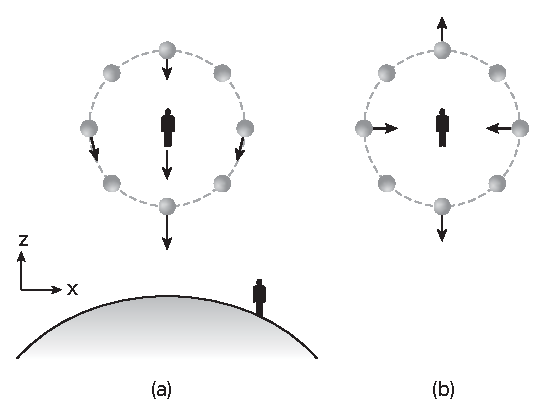
\includegraphics{tidal_of_falling_obj.eps}
	\caption{(a)为地面的观测者看空中的潮汐力,(b)为自由落体观测者参考系}
	\label{fig:tidal_of_falling_obj}
\end{figure}
如果我们将参考系变换到自由落体的物体上,那么我们自然会看到如图\ref{fig:tidal_of_falling_obj}(b)所示的潮汐力,参考系变换即把所有力减去中心粒子所受力即可。如果把自由落体参考系中的潮汐力图像化,即如图\ref{fig:tidal_of_moon}所示,我们可以看到这就是“潮汐”的经典的物理图像。
\begin{figure}[h]
	\centering
	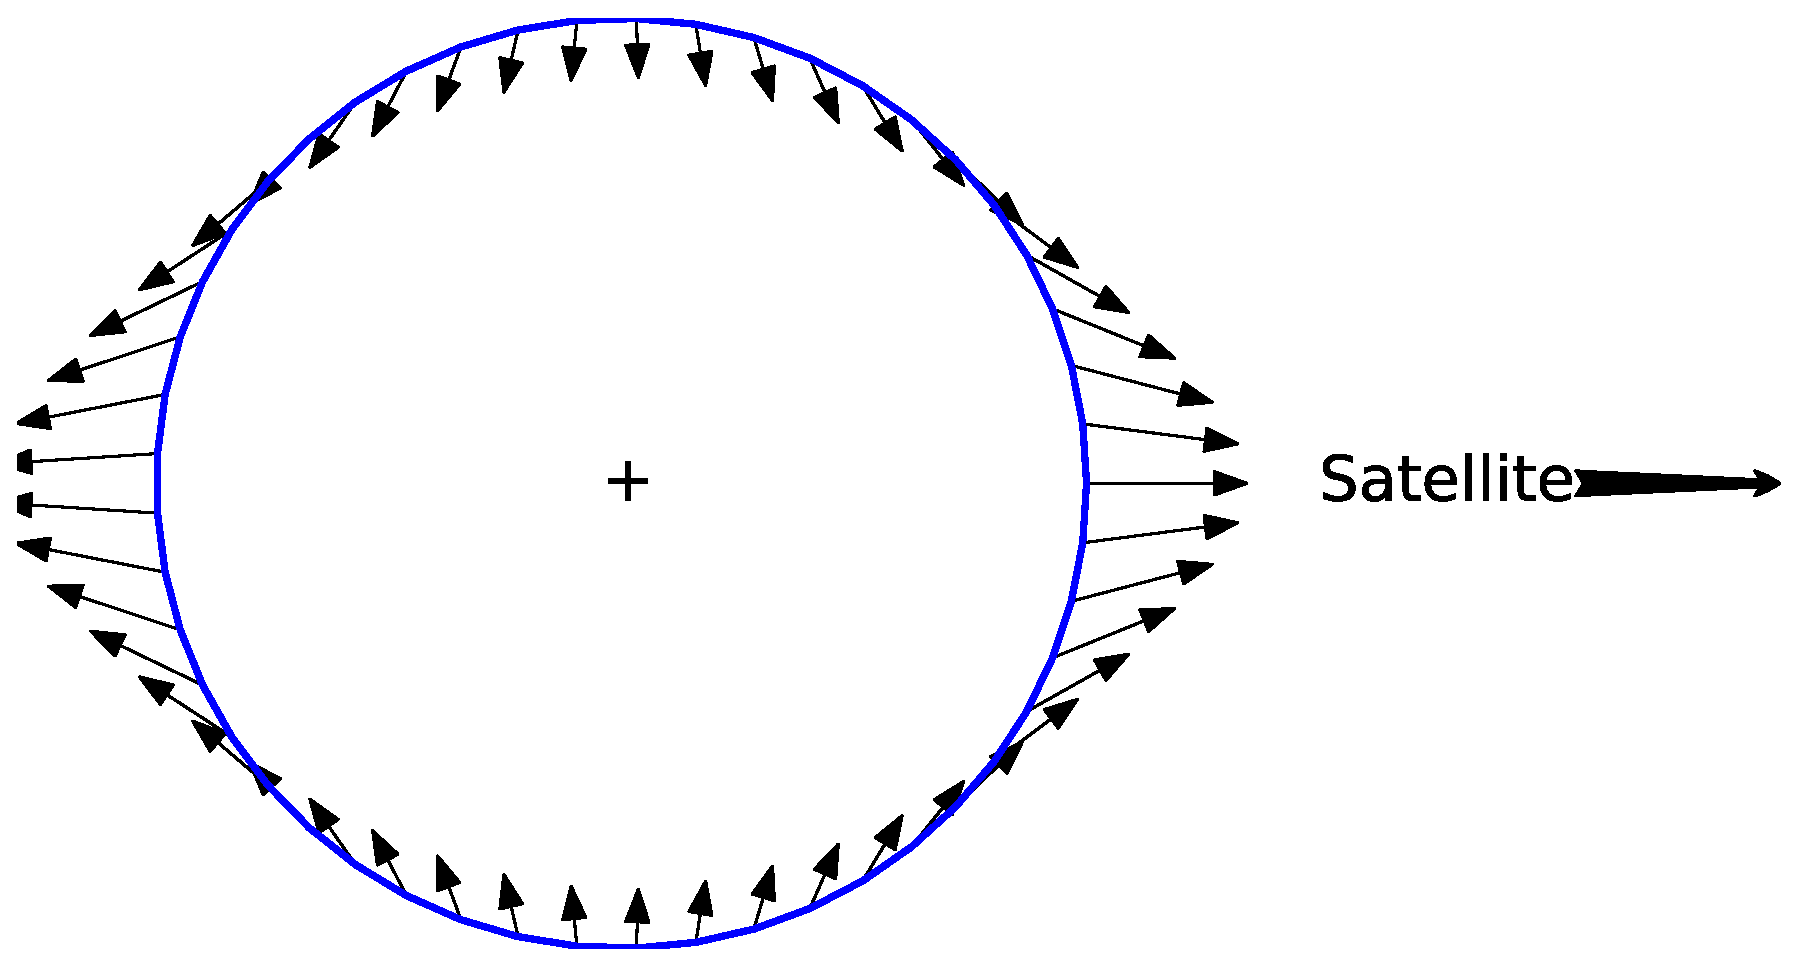
\includegraphics[scale=0.3]{tidal_of_moon.eps}
	\caption{月亮对地球的潮汐力场}
	\label{fig:tidal_of_moon}
\end{figure}
\subsubsection{测地偏移方程}
在广相的框架下,局域的自由粒子总沿着测地线运动,因此如果想要得到引力场的非均匀性,那么我们自然应当考虑两个沿无限接近测地线的自由粒子的运动。考虑两条接近的测地线$\gamma _{0} ,\gamma _{1}$,他们的参数化由$x^{\alpha }( t)$给出,其中$t$为仿射参数。这两条测地线可能是类时,类光或者类空的。类似于经典情景,我们想要获得一个关于这两条测地线的“偏移矢量”并且获得它的方程。如图\ref{eq:geodesic_cong}所示,我们在两条测地线中内插一族不相交的测地线,并用参数$s$标记这组测地线(后称测地线汇),即此测地线族为$x^{\alpha }( s,t)$,$s=0$时对应的测地线为$\gamma _{0}$,$s=1$对应的测地线为$\gamma _{1}$。

\begin{figure}
	\centering
	

\tikzset{every picture/.style={line width=0.75pt}} %set default line width to 0.75pt        

\begin{tikzpicture}[x=0.75pt,y=0.75pt,yscale=-1,xscale=1]
%uncomment if require: \path (0,174); %set diagram left start at 0, and has height of 174

%Curve Lines [id:da6599678366291943] 
\draw    (272.01,161.86) .. controls (302.01,132.86) and (267.01,42.86) .. (307.01,12.86) ;
%Curve Lines [id:da7243340632234556] 
\draw    (357.01,161.86) .. controls (387.01,132.86) and (352.01,42.86) .. (392.01,12.86) ;
%Curve Lines [id:da17659953985140864] 
\draw  [dash pattern={on 4.5pt off 4.5pt}]  (293.01,161.86) .. controls (323.01,132.86) and (288.01,42.86) .. (328.01,12.86) ;
%Curve Lines [id:da26658197592140453] 
\draw  [dash pattern={on 4.5pt off 4.5pt}]  (315.01,161.86) .. controls (345.01,132.86) and (310.01,42.86) .. (350.01,12.86) ;
%Curve Lines [id:da03377623956321174] 
\draw  [dash pattern={on 4.5pt off 4.5pt}]  (340.01,161.86) .. controls (370.01,132.86) and (335.01,42.86) .. (375.01,12.86) ;
%Curve Lines [id:da17887242348971033] 
\draw  [dash pattern={on 4.5pt off 4.5pt}]  (252.01,48.39) .. controls (265.01,25.39) and (379.01,24.39) .. (410.01,37.39) ;
%Curve Lines [id:da7269502507510239] 
\draw  [dash pattern={on 4.5pt off 4.5pt}]  (252.01,78.39) .. controls (265.01,55.39) and (379.01,54.39) .. (410.01,67.39) ;
%Curve Lines [id:da8226475847377916] 
\draw  [dash pattern={on 4.5pt off 4.5pt}]  (252.01,110.39) .. controls (265.01,87.39) and (379.01,86.39) .. (410.01,99.39) ;
%Curve Lines [id:da5703454617380816] 
\draw  [dash pattern={on 4.5pt off 4.5pt}]  (252.01,143.39) .. controls (265.01,120.39) and (379.01,119.39) .. (410.01,132.39) ;
%Straight Lines [id:da9561217469497414] 
\draw    (285.01,95.86) -- (283.08,45.86) ;
\draw [shift={(283.01,43.86)}, rotate = 447.8] [color={rgb, 255:red, 0; green, 0; blue, 0 }  ][line width=0.75]    (8.74,-2.63) .. controls (5.56,-1.12) and (2.65,-0.24) .. (0,0) .. controls (2.65,0.24) and (5.56,1.12) .. (8.74,2.63)   ;
%Straight Lines [id:da30666659441265054] 
\draw    (325.01,123.93) -- (390.01,122.96) ;
\draw [shift={(392.01,122.93)}, rotate = 539.14] [color={rgb, 255:red, 0; green, 0; blue, 0 }  ][line width=0.75]    (8.74,-2.63) .. controls (5.56,-1.12) and (2.65,-0.24) .. (0,0) .. controls (2.65,0.24) and (5.56,1.12) .. (8.74,2.63)   ;

% Text Node
\draw (279,2) node [anchor=north west][inner sep=0.75pt]    {$\gamma _{0}$};
% Text Node
\draw (393,0) node [anchor=north west][inner sep=0.75pt]    {$\gamma _{1}$};
% Text Node
\draw (262,42) node [anchor=north west][inner sep=0.75pt]    {$u^{\alpha }$};
% Text Node
\draw (394,107) node [anchor=north west][inner sep=0.75pt]    {$\xi ^{\alpha }$};
% Text Node
\draw (417,33) node [anchor=north west][inner sep=0.75pt]    {$s$};
% Text Node
\draw (235,150) node [anchor=north west][inner sep=0.75pt]    {$s=0$};
% Text Node
\draw (371,150) node [anchor=north west][inner sep=0.75pt]    {$s=1$};


\end{tikzpicture}
	\caption{测地线汇$x^{\alpha }( s,t)$}
	\label{eq:geodesic_cong}
\end{figure}
我们记测地线的切向量为$u^{\alpha } \equiv \partial x^{\alpha } /\partial t$,则我们的测地线方程自然可以写成:
\begin{equation*}
	u^{\alpha }{}_{;\beta } u^{\beta } =0
\end{equation*}
如果我们固定$t$而变动$s$,我们自然得到其他测地线。我们考虑这组测地线的切向量,即$\xi ^{\alpha } \equiv \partial x^{\alpha } /\partial s$。如果我们将$\xi ^{\alpha }$限制到$\gamma _{0}$上,即考虑$\xi ^{\alpha }| _{s=0}$,那么我们可以用此来表示$\gamma _{0}$和$\gamma _{1}$之间的偏差。类比于经典情况,我们自然应当考虑偏差$\xi ^{\alpha }$的“加速度”,即:
\begin{equation*}
	\begin{aligned}
		\frac{\mathrm{D}^{2} \xi ^{\alpha }}{\mathrm{d} t^{2}} & =\frac{\mathrm{D}}{\mathrm{d} t} ( \xi ^{\alpha }{}_{;\beta } u^{\beta } )=( \xi ^{\alpha }{}_{;\beta } u^{\beta } )_{;\gamma } u^{\gamma }
	\end{aligned}
\end{equation*}
在平直时空中,上式应当为$0$,因为平直时空的引力场均匀,两个粒子的测地线应当完全一致。如果上式不为$0$,那自然反映了时空弯曲的二阶效应,即曲率,实际上我们通过计算也可以得出上式正比于黎曼张量。如果我们将上式计算出来就得到了广相框架下的测地偏移方程。由定义:
\begin{equation*}
	u^{\alpha } =\frac{\partial x^{\alpha }}{\partial t} ,\xi ^{\alpha } =\frac{\partial x^{\alpha }}{\partial s} \Rightarrow u^{\alpha }{}_{;\beta } \xi ^{\beta } =\frac{\partial u^{\alpha }}{\partial s} =\frac{\partial ^{2} x^{\alpha }}{\partial t\partial s} =\frac{\partial \xi ^{\alpha }}{\partial t} =\xi ^{\alpha }{}_{;\beta } u^{\beta }
\end{equation*}
实际上,由直觉我们也可以看出$\xi ^{\alpha }$和$u^{\alpha }$是垂直的,如果计算一下:
\begin{equation*}
	\begin{aligned}
		\frac{\mathrm{d}}{\mathrm{d} t} ( \xi ^{\alpha } u_{\alpha } ) & =(\xi ^{\alpha } u_{\alpha } )_{;\beta } u^{\beta } =\xi ^{\alpha }{}_{;\beta } u_{\alpha } u^{\beta } +\xi ^{\alpha } u_{\alpha ;\beta } u^{\beta }\xlongequal{u_{\alpha ;\beta } u^{\beta } =0} u^{\alpha }{}_{;\beta } \xi ^{\beta } u_{\alpha } =\frac{1}{2} (u^{\alpha } u_{\alpha } )_{;\beta } \xi ^{\beta }
	\end{aligned}
\end{equation*}
但由于$u^{\alpha } u_{\alpha } \equiv \varepsilon $为一个常数,因此$\mathrm{d} (\xi ^{\alpha } u_{\alpha } )/\mathrm{d} t=0$。如果我们选取适当的参数,自然可以使$\xi ^{\alpha } u_{\alpha } =0$,因此$\xi ^{\alpha }$处处垂直于$u^{\alpha }$,这也进一步印证了$\xi ^{\alpha }$可以作为测量测地线“偏移”的量。

现在我们来计算“加速度”:
\begin{equation*}
	\begin{aligned}
		\frac{\mathrm{D}^{2} \xi ^{\alpha }}{\mathrm{d} t^{2}} & =(\xi ^{\alpha }{}_{;\beta } u^{\beta } )_{;\gamma } u^{\gamma }\\
		& =(u^{\alpha }{}_{;\beta } \xi ^{\beta } )_{;\gamma } u^{\gamma }\\
		& =u^{\alpha }{}_{;\beta \gamma } \xi ^{\beta } u^{\gamma } +u^{\alpha }{}_{;\beta } \xi ^{\beta }{}_{;\gamma } u^{\gamma }\\
		& =(u^{\alpha }{}_{;\gamma \beta } -R^{\alpha }{}_{\mu \beta \gamma } u^{\mu } )\xi ^{\beta } u^{\gamma } +u^{\alpha }{}_{;\beta } u^{\beta }{}_{;\gamma } \xi ^{\gamma }\\
		& =(u^{\alpha }{}_{;\gamma } u^{\gamma } )_{;\beta } \xi ^{\beta } -\textcolor[rgb]{0.82,0.01,0.11}{u^{\alpha }{}_{;\gamma } u^{\gamma }{}_{;\beta } \xi ^{\beta }} -R^{\alpha }{}_{\mu \beta \gamma } u^{\mu } \xi ^{\beta } u^{\gamma } +\textcolor[rgb]{0.29,0.56,0.89}{u^{\alpha }{}_{;\beta } u^{\beta }{}_{;\gamma } \xi ^{\gamma }}
	\end{aligned}
\end{equation*}
其中第四个等号采用了结论(有时黎曼张量也如此定义):
\begin{equation*}
	u^{\alpha }{}_{;\beta \gamma } -u^{\alpha }{}_{;\gamma \beta } =-R^{\alpha }{}_{\delta \beta \gamma } u^{\delta }
\end{equation*}
但由于测地线方程$u^{\alpha }{}_{;\gamma } u^{\gamma } =0$,因此我们得到了测地偏移方程:
\begin{equation}
	\boxed{\frac{\mathrm{D}^{2} \xi ^{\alpha }}{\mathrm{d} t^{2}} =-R^{\alpha }{}_{\mu \beta \gamma } u^{\mu } \xi ^{\beta } u^{\gamma }}
	\label{geodesic deviation}
\end{equation}
这个方程说明了曲率能造成两条相邻测地线的相对加速度,体现了引力场的“非均匀性”,也正因为此,有时我们也借助式\eqref{geodesic deviation}来定义黎曼张量。

\subsubsection{弱场近似}
一个好的理论必须在非相对论极限下回到牛顿力学,现在我们来看看在弱场近似下测地偏移方程\eqref{geodesic deviation}如何退化到\eqref{GD classic}。在弱场近似下,式\eqref{geodesic deviation}的左侧退化成$\mathrm{d}^{2} /\mathrm{d} t^{2}$,而$u^{\mu }\rightarrow \delta ^{\mu }{}_{0}$,因此我们有:
\begin{equation}
	\frac{\mathrm{d}^{2} \xi ^{\alpha }}{\mathrm{d} t^{2}} =-R^{\alpha }{}_{0\beta 0} \xi ^{\beta }
	\label{GD to cl}
\end{equation}
对比\eqref{GD to cl}和\eqref{GD classic},我们可以发现:
\begin{equation*}
	R^{i}{}_{0j0}\xrightarrow{\text{CL.}} R^{i}{}_{j} =g^{ik} \Phi _{;jk}
\end{equation*}
在球坐标下:
\begin{equation*}
	V( r) =-\frac{GM}{r} \Rightarrow V( r)_{;i} =\frac{GM}{r^{2}} \delta ^{r}{}_{i}
\end{equation*}
为了计算下一步协变导数,我们需要球坐标下的克氏符的$r$分量:\begin{equation*}
	\Gamma ^{r}{}_{\theta \theta } =-r,\Gamma ^{r}{}_{\phi \phi } =-r\sin^{2} \theta 
\end{equation*}

因此我们有:
\begin{equation*}
	V( r)_{;ij} =\partial _{i} \partial _{j} V-\Gamma ^{k}{}_{ij} \partial _{k} V=-\frac{2GM}{r^{3}} \delta ^{r}{}_{i} \delta ^{r}{}_{j} -\Gamma ^{r}{}_{ij}\frac{GM}{r^{2}}
\end{equation*}
故
\begin{equation*}
	R_{11} =-\frac{2GM}{r^{3}} ,R_{22} =\frac{GM}{r} ,R_{33} =\sin^{2} \theta \frac{GM}{r}
\end{equation*}
那么我们需要证明的东西在球坐标下就变成了:
\begin{equation*}
	R^{1}{}_{010}\rightarrow R^{1}{}_{1} =-\frac{2GM}{r^{3}} ,R^{2}{}_{020}\rightarrow R^{2}{}_{2} =\frac{GM}{r^{3}} ,R^{3}{}_{030}\rightarrow R^{3}{}_{3} =\frac{GM}{r^{3}}
\end{equation*}
在牛顿极限下,我们设$g_{\mu \nu } =\eta _{\mu \nu } +h_{\mu \nu }$,对比测地偏移方程和牛顿第二定律我们有:
\begin{equation*}
	h_{00} =-2V\Rightarrow g_{00} =-1+\frac{2GM}{r}
\end{equation*}
那么我们对此度规计算黎曼张量,得到:
\begin{equation*}
	R^{1}{}_{010} =\frac{GM( -3GM+2r)}{( 2GM-r) r^{3}}\xrightarrow{r\gg GM} -\frac{2GM}{r^{3}} ,R^{2}{}_{020} =R^{3}{}_{030} =\frac{GM}{r^{3}} \ 
\end{equation*}
因此测地偏移方程在经典极限下的确退化为了牛顿引力的结果。

\subsection{Raychaudhuri 方程}

经典力学里,我们常常更关注一个质点在给定时空背景下的运动轨迹,而并不太关注一族质点的运动轨迹相互之间的关系(经典情况下,这属于连续介质力学或流体力学研究的范畴)。但当我们考虑广义相对论的时候,物体的运动取决于时空本身的(几何)性质,反之我们自然也可以通过研究物体的运动轨迹来观察时空的几何特性。但与牛顿力学的各向同性的平直时空不同,弯曲时空中,仅仅研究一个质点会如何运动是不够的,如果我们要观察时空某个区域的性质,我们必须考虑一族质点会如何运动,也就是一组测地线汇。



作为引入,我们首先考虑经典力学框架下的二维可压缩介质的内部运动。


\subsubsection{经典流体}
\paragraph{二维情况}

考虑一个二维可形变流体,如图\ref{fig:classic_fluid}所示。

\begin{figure}
	\centering
	
\tikzset{every picture/.style={line width=0.75pt}} %set default line width to 0.75pt        

\begin{tikzpicture}[x=0.75pt,y=0.75pt,yscale=-1,xscale=1]
	%uncomment if require: \path (0,234); %set diagram left start at 0, and has height of 234
	
	%Shape: Polygon Curved [id:ds22637236277951622] 
	\draw   (247.37,40.6) .. controls (262.37,30.6) and (378.37,28.6) .. (399.37,39.6) .. controls (420.37,50.6) and (411.37,61.6) .. (394.37,64.6) .. controls (377.37,67.6) and (264.37,68.6) .. (251.37,63.6) .. controls (238.37,58.6) and (232.37,50.6) .. (247.37,40.6) -- cycle ;
	%Curve Lines [id:da18689240443569588] 
	\draw    (274,13) .. controls (279.37,25.6) and (279.37,40.6) .. (279.37,53.6) ;
	%Curve Lines [id:da17346503975046823] 
	\draw    (280.37,66.6) .. controls (280.37,84.6) and (284.37,144.6) .. (283.37,153.6) ;
	%Shape: Polygon Curved [id:ds6361529811634252] 
	\draw   (257.37,138.6) .. controls (272.37,128.6) and (388.37,126.6) .. (409.37,137.6) .. controls (430.37,148.6) and (421.37,159.6) .. (404.37,162.6) .. controls (387.37,165.6) and (274.37,166.6) .. (261.37,161.6) .. controls (248.37,156.6) and (242.37,148.6) .. (257.37,138.6) -- cycle ;
	%Curve Lines [id:da06818232449983341] 
	\draw    (283,166) .. controls (281.37,184.47) and (282.37,215.47) .. (270.37,219.47) ;
	%Curve Lines [id:da734723595223542] 
	\draw    (365.2,13) .. controls (359.83,25.6) and (359.83,40.6) .. (359.83,53.6) ;
	%Curve Lines [id:da23344765681601598] 
	\draw    (358.83,66.6) .. controls (358.83,84.6) and (356.37,146.6) .. (357.37,155.6) ;
	%Curve Lines [id:da34374856442148904] 
	\draw    (357.2,165) .. controls (357.37,184.6) and (362.37,214.6) .. (370.37,220.6) ;
	%Straight Lines [id:da7895975283807535] 
	\draw    (285.37,154.6) -- (355.37,155.57) ;
	\draw [shift={(357.37,155.6)}, rotate = 180.8] [fill={rgb, 255:red, 0; green, 0; blue, 0 }  ][line width=0.08]  [draw opacity=0] (12,-3) -- (0,0) -- (12,3) -- cycle    ;
	
	% Text Node
	\draw (285,44) node [anchor=north west][inner sep=0.75pt]    {$O$};
	% Text Node
	\draw (371,44) node [anchor=north west][inner sep=0.75pt]    {$P$};
	% Text Node
	\draw (259.37,141.6) node [anchor=north west][inner sep=0.75pt]    {$O$};
	% Text Node
	\draw (372,142) node [anchor=north west][inner sep=0.75pt]    {$P$};
	% Text Node
	\draw (323,133) node [anchor=north west][inner sep=0.75pt]    {$\xi ^{a}$};
	% Text Node
	\draw (366,69) node [anchor=north west][inner sep=0.75pt]    {$t=t_{1}$};
	% Text Node
	\draw (366.2,169) node [anchor=north west][inner sep=0.75pt]    {$t=t_{0}$};
	
	
\end{tikzpicture}
	\caption{经典情况下的二维可压缩流体}
	\label{fig:classic_fluid}
\end{figure}

对于相对于$O$点的微小形变$\xi ^{a}$,我们可以写下:
\begin{equation*}
	\frac{\mathrm{d} \xi ^{a}}{\mathrm{d} t} =B^{a}{}_{b}( t) \xi ^{b} +O \left( \xi ^{2}\right)
\end{equation*}
其中$B^{a}{}_{b}$为一个张量。此张量与时间的关系由该流体的动力学确定。对于一个很小的时间间隔,我们有:
\begin{equation*}
	\xi ^{a}( t_{1}) =\xi ^{a}( t_{0}) +\Delta \xi ^{a}( t_{0})
\end{equation*}
其中
\begin{equation*}
	\Delta \xi ^{a} =B^{a}{}_{b}( t_{0}) \xi ^{b}( t_{0}) \Delta t+O \left( \Delta t^{2}\right) ,\Delta t=t_{1} -t_{0} .
\end{equation*}
现在我们考虑$B^{a}{}_{b}$的具体形式。首先讨论一个非常简单的图像:$\xi ^{a}( t_{0}) =r_{0}(\cos \phi ,\sin \phi )$。由于$B^{a}{}_{b}$为一个二阶张量,最多有四个独立分量,可以被分解为无迹对称部分,反对称部分和迹的部分。我们可以分别就这三种情况讨论$B$的作用,最后即可获得一般情况。
\begin{itemize}
\item 假设$B^{a}{}_{b}$正比与单位阵,即
\begin{equation*}
	B^{a}{}_{b} =\frac{1}{2}\begin{pmatrix}
		\theta  & 0\\
		0 & \theta 
	\end{pmatrix}
\end{equation*}

我们有$\theta \equiv B^{a}{}_{a}$,则$\Delta \xi ^{a} =\frac{1}{2} \theta r_{0} \Delta t(\cos \phi ,\sin \phi )$,这对应了圆的半径的变化:$r_{1} =r_{0} +\frac{1}{2} \theta r_{0} \Delta t$。那么对应的区域的面积变化显然是$\Delta A=A_{1} -A_{0} =\pi r_{0}^{2} \theta \Delta t$,因此
\begin{equation*}
	\theta =\frac{1}{A_{0}}\frac{\Delta A}{\Delta t}
\end{equation*}

其中参数$\theta $可以被视为单位时间内区域面积的变化,因此被称为膨胀参数(expansion parameter)。实际上,由于$\theta $取决于时间和参考点$O$,因此它其实是一个函数。
\item 假设$B^{a}{}_{b}$是对称且无迹的,即
\begin{equation*}
	B^{a}{}_{b} =\begin{pmatrix}
		\sigma _{+} & \sigma _{\times }\\
		\sigma _{\times } & -\sigma _{+}
	\end{pmatrix}
\end{equation*}

那么我们有
\begin{equation*}
	\Delta \xi ^{a} =r_{0} \Delta t( \sigma _{+}\cos \phi +\sigma _{\times }\sin \phi ,-\sigma _{+}\sin \phi +\sigma _{\times }\cos \phi )
\end{equation*}

我们可以得到新的半径为
\begin{equation*}
	r_{1}( \phi ) =r_{0}( 1+\sigma _{+} \Delta t\cos 2\phi +\sigma _{\times } \Delta t\sin 2\phi )
\end{equation*}

如果$\sigma _{\times } =0$,它代表了一个主轴沿着$\phi =0$方向的椭圆;而若$\sigma _{+} =0$,则代表了一个主轴沿着$\phi =\pi /4$方向的椭圆,如图\ref{fig:shear_effect}所示。

\begin{figure}
	\centering
	\tikzset{every picture/.style={line width=0.75pt}} %set default line width to 0.75pt        

\begin{tikzpicture}[x=0.75pt,y=0.75pt,yscale=-1,xscale=1]
	%uncomment if require: \path (0,157); %set diagram left start at 0, and has height of 157
	
	%Shape: Axis 2D [id:dp29866176738130945] 
	\draw  (94,70.99) -- (267.37,70.99)(181.29,10.5) -- (181.29,126.37) (260.37,65.99) -- (267.37,70.99) -- (260.37,75.99) (176.29,17.5) -- (181.29,10.5) -- (186.29,17.5)  ;
	%Shape: Circle [id:dp40113413830915556] 
	\draw  [dash pattern={on 0.84pt off 2.51pt}] (147.61,70.99) .. controls (147.61,52.39) and (162.69,37.31) .. (181.29,37.31) .. controls (199.9,37.31) and (214.98,52.39) .. (214.98,70.99) .. controls (214.98,89.6) and (199.9,104.68) .. (181.29,104.68) .. controls (162.69,104.68) and (147.61,89.6) .. (147.61,70.99) -- cycle ;
	%Shape: Ellipse [id:dp1244409331683014] 
	\draw   (120.11,70.99) .. controls (120.11,56.87) and (147.5,45.43) .. (181.29,45.43) .. controls (215.09,45.43) and (242.48,56.87) .. (242.48,70.99) .. controls (242.48,85.11) and (215.09,96.56) .. (181.29,96.56) .. controls (147.5,96.56) and (120.11,85.11) .. (120.11,70.99) -- cycle ;
	
	%Shape: Axis 2D [id:dp7244743980427475] 
	\draw  (376,70.99) -- (549.37,70.99)(463.29,10.5) -- (463.29,126.37) (542.37,65.99) -- (549.37,70.99) -- (542.37,75.99) (458.29,17.5) -- (463.29,10.5) -- (468.29,17.5)  ;
	%Shape: Circle [id:dp696594152216014] 
	\draw  [dash pattern={on 0.84pt off 2.51pt}] (429.61,70.99) .. controls (429.61,52.39) and (444.69,37.31) .. (463.29,37.31) .. controls (481.9,37.31) and (496.98,52.39) .. (496.98,70.99) .. controls (496.98,89.6) and (481.9,104.68) .. (463.29,104.68) .. controls (444.69,104.68) and (429.61,89.6) .. (429.61,70.99) -- cycle ;
	%Shape: Ellipse [id:dp2989551162692037] 
	\draw   (506.56,27.73) .. controls (516.54,37.71) and (505.27,65.18) .. (481.37,89.07) .. controls (457.48,112.96) and (430.02,124.24) .. (420.03,114.26) .. controls (410.05,104.27) and (421.32,76.81) .. (445.22,52.92) .. controls (469.11,29.02) and (496.57,17.75) .. (506.56,27.73) -- cycle ;
	
	
	% Text Node
	\draw (158,130.5) node [anchor=north west][inner sep=0.75pt]    {$\sigma _{\times } =0$};
	% Text Node
	\draw (440,130.5) node [anchor=north west][inner sep=0.75pt]    {$\sigma _{+} =0$};
	
	
\end{tikzpicture}
	\caption{切变张量的效果}
	\label{fig:shear_effect}
\end{figure}

也因此,$\sigma _{+} ,\sigma _{\times }$被称为切变参数(shear parameters)。
\item 如果$B^{a}{}_{b}$为反对称的,那么我们可以写下
\begin{equation*}
	B^{a}{}_{b} =\begin{pmatrix}
		0 & \omega \\
		-\omega  & 0
	\end{pmatrix}
\end{equation*}

那么我们有
\begin{equation*}
	\Delta \xi ^{a} =r_{0} \omega \Delta t(\sin \phi ,-\cos \phi ) ,\xi ^{a} =r_{0}(\cos \phi ',\sin \phi ') ,\phi '=\phi -\omega \Delta t
\end{equation*}

这很显然是一个旋转,因此我们也称$\omega $为涡旋参数(rotation parameter)。
\end{itemize}



那么对于一般情况,我们可以写下:
\begin{equation*}
B^{a}{}_{b} =\frac{1}{2}\begin{pmatrix}
	\theta  & 0\\
	0 & \theta 
\end{pmatrix} +\begin{pmatrix}
	\sigma _{+} & \sigma _{\times }\\
	\sigma _{\times } & -\sigma _{+}
\end{pmatrix} +\begin{pmatrix}
	0 & \omega \\
	-\omega  & 0
\end{pmatrix}
\end{equation*}
或者
\begin{equation*}
B_{ab} =\frac{1}{2} \theta \delta _{ab} +\sigma _{ab} +\omega _{ab}
\end{equation*}
其中
\begin{equation*}
\theta =B^{a}{}_{a} ,\sigma _{ab} =B_{( ab)} -\frac{1}{2} \theta \delta _{ab} ,\omega _{ab} =B_{[ ab]} .
\end{equation*}
\paragraph{三维情况}

类比二维情况,我们可以同样得出:
\begin{equation*}
B_{ab} =\frac{1}{3} \theta \delta _{ab} +\sigma _{ab} +\omega _{ab}
\end{equation*}
其中
\begin{equation*}
\theta =B^{a}{}_{a} ,\sigma _{ab} =B_{( ab)} -\frac{1}{3} \theta \delta _{ab} ,\omega _{ab} =B_{[ ab]} .
\end{equation*}
只不过在三维情况下,$\theta $为体积的变化率,即
\begin{equation*}
\theta =\frac{1}{V}\frac{\Delta V}{\Delta t}
\end{equation*}
因为如果我们把关系
\begin{equation*}
\xi ^{a}( t_{1}) =(\delta ^{a}{}_{b} +B^{a}{}_{b} \Delta t)\xi ^{b}( t_{0})
\end{equation*}
视作一个从$\xi ^{a}( t_{0})$到$\xi ^{b}( t_{1})$的坐标变换,那么其雅克比行列式为
\begin{equation*}
J=\det (\delta ^{a}{}_{b} +B^{a}{}_{b} \Delta t)=1+\operatorname{tr} (B^{a}{}_{b} \Delta t)=1+\theta \Delta t.
\end{equation*}
那么我们自然有
\begin{equation*}
V_{0} \theta =\frac{V_{1} -V_{0}}{\Delta t} .
\end{equation*}
这也意味着体积不受剪切和旋转的影响。

\subsubsection{类时测地线汇}

现在我们回到广义相对论框架。我们已经知道,曲率会导致沿相邻测地线运动的质点之间的距离发生变化,即所谓的测地偏离 (geodesic deviation) 效应。 现在,我们可以考虑一群质点在一组测地线下的运动。所谓线汇(congruence)就是在时空中的一个开区域$\mathscr{O}$中的一族穿过且仅穿过$\mathscr{O}$中每一点一次的一族曲线,且这些曲线不能相交。这里我们讨论类时测地线汇,观察一族类时测地线如何随时间变化,更具体的说,是两条测地线之间的测地偏移矢量$\xi ^{\alpha }$的行为。选取与测地偏移方程一节同样的记号,即切向量为$u^{\alpha } \equiv \partial x^{\alpha } /\partial t$,$\xi ^{\alpha } \equiv \partial x^{\alpha } /\partial s$为测地偏移矢量。选取适当的归一化,我们有:
\begin{equation*}
	u^{\alpha } u_{\alpha } =-1,u^{\alpha }{}_{;\beta } u^{\beta } =0,u^{\alpha }{}_{;\beta } \xi ^{\beta } =\xi ^{\alpha }{}_{;\beta } u^{\beta } ,u^{\alpha } \xi _{\alpha } =0
\end{equation*}
其中第一个式子是由于$u^{\alpha }$为类时的,二式则是测地线方程,四式则由$u^{\alpha }$和$\xi _{\alpha }$互相垂直的定义可以看出,因此我们也常说$\xi ^{\alpha }$指向于垂直于(transverse)这组线汇生成的流的方向。



随后,我们便可以根据这组线汇将度规$g_{\alpha \beta }$分解为竖直(longitudinal)部分$-u_{\alpha } u_{\beta }$与横向(transverse)部分$h_{\alpha \beta }$,即
\begin{equation*}
	h_{\alpha \beta } =g_{\alpha \beta } +u_{\alpha } u_{\beta }
\end{equation*}
注意,这里的横向度规只有“空间部分”,因为
\begin{equation*}
	u^{\alpha } h_{\alpha \beta } =u^{\alpha } g_{\alpha \beta } +u^{\alpha } u_{\alpha } u_{\beta } =u_{\beta } -u_{\beta } =0=h_{\alpha \beta } u^{\beta } ,
\end{equation*}
同时它也只有三个独立分量,因为如果我们考虑共动的4-洛伦兹标架,在此坐标系中我们有
\begin{equation*}
	u_{\alpha } =( -1,0,0,0) ,g_{\alpha \beta } =\operatorname{diag}( -1,1,1,1) ,h_{\alpha \beta } =( 0,1,1,1) .
\end{equation*}
同时我们还有$h^{\alpha }{}_{\mu } h^{\mu }{}_{\beta } =h^{\alpha }{}_{\beta }$.



类比经典情况,我们可以定义一个协变的张量:
\begin{equation*}
	B_{\alpha \beta } =u_{\alpha ;\beta }
\end{equation*}
与$h_{\alpha \beta }$相同,这个张量也是纯“横向”的,因为
\begin{equation*}
	u^{\alpha } B_{\alpha \beta } =u^{\alpha } u_{\alpha ;\beta } =\frac{1}{2} (u^{\alpha } u_{a} )_{;\beta } =0,B_{\alpha \beta } u^{\beta } =u_{\alpha ;\beta } u^{\beta } =0
\end{equation*}
因此,现在我们就有了测地偏移矢量的变化量,即
\begin{equation*}
	\xi ^{\alpha }{}_{;\beta } u^{\beta } =u^{\alpha }{}_{;\beta } \xi ^{\beta } =B^{\alpha }{}_{\beta } \xi ^{\beta } .
\end{equation*}
类比测地线方程$u^{\alpha }{}_{;\beta } u^{\beta } =0$可以看出,实际上$B^{\alpha }{}_{\beta }$度量了$\xi ^{\alpha }$沿着测地线平行移动的“失败程度”。



与经典的情况完全类似,我们可以将张量$B_{\alpha \beta }$分解为三部分,即
\begin{equation*}
	B_{\alpha \beta } =\frac{1}{3} \theta h_{\alpha \beta } +\sigma _{\alpha \beta } +\omega _{\alpha \beta }
\end{equation*}
其中$\theta =B^{\alpha }{}_{\alpha } =u^{\alpha }{}_{;\alpha }$被称为膨胀标量(expansion scalar),$\sigma _{\alpha \beta } =B_{( \alpha \beta )} -\frac{1}{3} \theta h_{\alpha \beta }$被称为切变张量 (shear tensor)以及$\omega _{\alpha \beta } =B_{[ \alpha \beta ]}$被称为涡旋张量(rotation tensor)。这些量的物理解释与经典情况下几乎一样。显然,如果$\theta  >0$,那么这组线汇是发散的,反之$\theta < 0$,这组测地线则是汇聚的。


\paragraph{Frobenius 定理}

如果涡旋张量为零,即$\omega _{\alpha \beta } =0$,这样的线汇被称为超曲面正交的(hypersurface orthogonal)的,意思是对于这个线汇,处处都有一族超曲面与每一点的曲线垂直,如图\ref{fig:hypersurface_orthogonal}所示。

\begin{figure}
	\centering
	\tikzset{every picture/.style={line width=0.75pt}} %set default line width to 0.75pt        

\begin{tikzpicture}[x=0.75pt,y=0.75pt,yscale=-1,xscale=1]
	%uncomment if require: \path (0,243); %set diagram left start at 0, and has height of 243
	
	%Straight Lines [id:da9375970960458557] 
	\draw    (194,114.24) -- (465.37,114.24) ;
	%Straight Lines [id:da7808160969606883] 
	\draw    (329.37,222.26) -- (328.37,5.26) ;
	%Curve Lines [id:da7351197655463686] 
	\draw    (248.37,15.52) .. controls (272.37,60.52) and (291.37,130.52) .. (247.37,213.26) ;
	%Curve Lines [id:da9732510461282793] 
	\draw    (193.37,76.52) .. controls (269.37,33.52) and (370.37,24.52) .. (465.37,78.26) ;
	%Curve Lines [id:da27633094958530524] 
	\draw    (408.37,212.26) .. controls (384.37,167.26) and (365.37,97.26) .. (409.37,14.52) ;
	%Curve Lines [id:da5645890455124096] 
	\draw    (464.37,150.26) .. controls (388.37,193.26) and (287.37,202.26) .. (192.37,148.52) ;
	
	
	% Text Node
	\draw (237,210) node [anchor=north west][inner sep=0.75pt]    {$\gamma _{1}$};
	% Text Node
	\draw (322,221) node [anchor=north west][inner sep=0.75pt]    {$\gamma _{2}$};
	% Text Node
	\draw (405,211) node [anchor=north west][inner sep=0.75pt]    {$\gamma _{3}$};
	% Text Node
	\draw (466,134) node [anchor=north west][inner sep=0.75pt]    {$\Sigma _{1}$};
	% Text Node
	\draw (467,98) node [anchor=north west][inner sep=0.75pt]    {$\Sigma _{2}$};
	% Text Node
	\draw (468,62) node [anchor=north west][inner sep=0.75pt]    {$\Sigma _{3}$};
	
	
\end{tikzpicture}
	\caption{与测地线汇正交的超曲面族}
	\label{fig:hypersurface_orthogonal}
\end{figure}


这被称为Frobenius定理。下面我们给出这个定理证明的一些步骤。如果一个线汇是超曲面正交的,那么其切向量$u^{\alpha }$应当处处正比于超曲面的法向量$n^{\alpha }$。设这些超曲面被方程$\Phi (x^{\alpha } )=c$所描述,那么由于$n_{\alpha } \varpropto \Phi _{,\alpha }$,那么我们可以有
\begin{equation*}
	u_{\alpha } =-\mu \Phi _{,\alpha }
\end{equation*}
其中$\mu $是正比系数。这里我们假设$\Phi $是朝着未来增加的,那么由于$u^{\alpha } u_{\alpha } =-1$我们可以看出$\mu $是正数。对此方程求协变导数,我们有
\begin{equation*}
	u_{\alpha ;\beta } =-\mu \Phi _{;\alpha \beta } -\Phi _{,\alpha } \mu _{,\beta }
\end{equation*}
现在定义以下反对称张量:
\begin{equation*}
	u_{[ \alpha ;\beta } u_{\gamma ]} \equiv \frac{1}{3!}( u_{\alpha ;\beta } u_{\gamma } +u_{\gamma ;\alpha } u_{\beta } +u_{\beta ;\gamma } u_{\alpha } -u_{\beta ;\alpha } u_{\gamma } -u_{\alpha ;\gamma } u_{\beta } -u_{\gamma ;\beta } u_{\alpha })
\end{equation*}
但由于$\Phi _{;\beta ;\alpha } =\Phi _{;\alpha ;\beta }$,我们可以得出上式右侧为零,即超曲面正交可以推出$u_{[ \alpha ;\beta } u_{\gamma ]} =0$。反过来,如果$u_{[ \alpha ;\beta } u_{\gamma ]} =0$,我们也可以推出存在一个场$\Phi $,使得$u_{\alpha } \varpropto \Phi _{,\alpha }$,但证明更加繁琐。这一对正题和反题被称为Frobenius定理。注意,由于前面我们并没有用到测地线方程,因此实际上这个定理对任何线汇都成立。

如果此线汇为测地线汇,那么我们可以计算:
\begin{equation*}
	\begin{aligned}
		3!u_{[ \alpha ;\beta } u_{\gamma ]} & =2( u_{[ \alpha ;\beta ]} u_{\gamma } +u_{[ \gamma ;\alpha ]} u_{\beta } +u_{[ \beta ;\gamma ]} u_{\alpha })\\
		& =2( B_{[ \alpha \beta ]} u_{\gamma } +B_{[ \gamma \alpha ]} u_{\beta } +B_{[ \beta \gamma ]} u_{\alpha })\\
		& =2( \omega _{\alpha \beta } u_{\gamma } +\omega _{\gamma \alpha } u_{\beta } +\omega _{\beta \gamma } u_{\alpha })
	\end{aligned}
\end{equation*}
如果$u_{[ \alpha ;\beta } u_{\gamma ]} =0$,我们显然有$\omega _{\alpha \beta } =0$,即一开始我们所说的条件。注意,此情况仅对类时测地线成立,而$u_{[ \alpha ;\beta } u_{\gamma ]} =0$对一般的线汇都成立。

同时注意到$\mu $在同样的超曲面上是一个常数,因此我们可以将$\mu $视为$\Phi $的函数。如果我们定义
\begin{equation*}
	\Psi \equiv \int \mu ( \Phi )\mathrm{d} \Phi 
\end{equation*}
则我们有$u_{\alpha } =-\Psi _{,\alpha }$。同时注意到,如果$u_{\alpha }$可以被这种形式表达,那么它其实自动满足了测地线方程:
\begin{equation*}
	u_{\alpha ;\beta } u^{\beta } =\Psi _{;\alpha \beta } \Psi ^{,\beta } =\Psi _{;\beta \alpha } \Psi ^{,\beta } =\frac{1}{2} (\Psi ^{,\beta } \Psi _{,\beta } )_{;\alpha } =\frac{1}{2} (u^{\beta } u_{\beta } )_{;\alpha } =0
\end{equation*}
我们对上述结果做个总结:
\begin{center}
	\begin{tabular}{|c|c|c|}
		\hline
		& 任意矢量场$u^{\alpha }$ & 类时测地线 \\
		\hline
		超曲面正交的条件 & $\exists \Phi ,u_{\alpha } \varpropto \Phi _{,\alpha }$ & $\exists \Psi ,u_{\alpha } =-\Psi _{,\alpha } ,\omega _{\alpha \beta } =u_{[ \alpha ;\beta ]} =0$ \\
		\hline
	\end{tabular}
\end{center}

\paragraph{Raychaudhuri 方程}

现在我们考虑膨胀标量$\theta $随时间的变化。考虑:
\begin{equation*}
	\begin{aligned}
		B_{\alpha \beta ;\mu } u^{\mu } & =u_{\alpha ;\beta ;\mu } u^{\mu }\\
		& =(u_{\alpha ;\mu ;\beta } -R_{\alpha \nu \beta \mu } u^{\nu } )u^{\mu }\\
		& =(u_{\alpha ;\mu } u^{\mu } )_{;\beta } -u_{\alpha ;\mu } u^{\mu }{}_{;\beta } -R_{\alpha \nu \beta \mu } u^{\nu } u^{\mu }\\
		& =-B_{\alpha \mu } B^{\mu }{}_{\beta } -R_{\alpha \nu \beta \mu } u^{\nu } u^{\mu }
	\end{aligned}
\end{equation*}
那么我们有:
\begin{equation*}
	\frac{\mathrm{d} \theta }{\mathrm{d} \tau } =\frac{\mathrm{d}}{\mathrm{d} \tau } B_{\alpha \beta } g^{\alpha \beta } =B_{\alpha \beta ;\mu } u^{\mu } g^{\alpha \beta } =B^{\alpha }{}_{\alpha ;\mu } u^{\mu } =-B^{\alpha \beta } B_{\beta \alpha } -R_{\alpha \beta } u^{\alpha } u^{\beta }
\end{equation*}
注意到
\begin{equation*}
	\begin{aligned}
		B^{\alpha \beta } B_{\beta \alpha } & =\left(\frac{1}{3} \theta h^{\alpha \beta } +\sigma ^{\alpha \beta } +\omega ^{\alpha \beta }\right)\left(\frac{1}{3} \theta h_{\beta \alpha } +\sigma _{\beta \alpha } +\omega _{\beta \alpha }\right)\\
		& =\frac{1}{9} \theta ^{2} h^{\alpha \beta } h_{\alpha \beta } +\sigma ^{a\beta } \sigma _{\alpha \beta } +\omega ^{\alpha \beta } \omega _{\beta \alpha }\\
		& =\frac{1}{3} \theta ^{2} h^{\alpha \beta } h_{\alpha \beta } +\sigma ^{a\beta } \sigma _{\alpha \beta } -\omega ^{\alpha \beta } \omega _{\alpha \beta }
	\end{aligned}
\end{equation*}
故我们得到了对于类时测地线的Raychaudhuri方程,即
\begin{equation*}
	\boxed{\frac{\mathrm{d} \theta }{\mathrm{d} \tau } =-\frac{1}{3} \theta ^{2} -\sigma ^{a\beta } \sigma _{\alpha \beta } +\omega ^{\alpha \beta } \omega _{\alpha \beta } -R_{\alpha \beta } u^{\alpha } u^{\beta }}
\end{equation*}
注意到切变和涡旋张量都为纯空间的(即时间分量为0,有效度规为欧式度规),因此$\sigma ^{\alpha \beta } \sigma _{\alpha \beta } \geq 0$且$\omega ^{\alpha \beta } \omega _{\alpha \beta } \geq 0$。等号在该张量恰好为零的时候成立。


\paragraph{汇聚定理}

现在,如果我们假设该类时测地线汇是超曲面垂直的,即$\omega _{\alpha \beta } =0$,且强能量条件成立,即$R_{\alpha \beta } u^{\alpha } u^{\beta } \geq 0$,那么我们有
\begin{equation*}
	\frac{\mathrm{d} \theta }{\mathrm{d} \tau } =-\frac{1}{3} \theta ^{2} -\sigma ^{a\beta } \sigma _{\alpha \beta } -R_{\alpha \beta } u^{\alpha } u^{\beta } \leq 0
\end{equation*}
即膨胀参数随着测地线的演化而逐渐减小。因此一个一开始发散($\theta  >0$)的测地线汇会逐渐收敛,而一个原本收敛($\theta < 0$)的测地线汇会收敛地更快,这就是所谓的汇聚定理(focusing theorem)。

同时我们可以看出
\begin{equation*}
	\frac{\mathrm{d} \theta }{\mathrm{d} \tau } \leq -\frac{1}{3} \theta ^{2} \Rightarrow \theta ^{-1}( \tau ) \geq \theta {_{0}}^{-1} +\frac{\tau }{3}
\end{equation*}
其中$\theta _{0} \equiv \theta ( 0)$。显然,如果此测地线汇本来是收敛的,即$\theta _{0} < 0$,那么在有限的固有时$\tau \leq 3/| \theta _{0}| $内,$\theta ( \tau )\rightarrow -\infty $,即测地线会汇聚到一点,这被称为汇聚点(caustic),此时测地偏移矢量场——也称为 Jacobi 场 (Jacobi field)——在该处为零。注意,汇聚点只是一个抽象的几何性质, 不会直接导致奇点(singularity)的产生。至于什么是奇点,后文会做详细说明。



如果一个从$p$点发出的类时测地线汇在$q$点汇聚,我们就把$q$和$p$称为该测地线汇上的一对共轭点 (conjugate points)。 从上面的分析中我们看到, 如果从$p$点发出的一个类时测地线汇在未来某一点上出现汇聚效应$\theta < 0$, 则在该线汇上距离$p$有限远的地方必定存在一个与$p$共轭的点$q$——当然,这里我们要假定该测地线汇可以延伸到$q$点。



在一个测地完备时空中, “测地线束可以延伸到$q$点” 这一假定是自动满足的。注意到,即使$\sigma _{\alpha \beta } \sigma ^{\alpha \beta }$与$R_{\alpha \beta } u^{\alpha } u^{\beta }$处处为零,且在$\theta _{0}  >0$这一对于形成$\theta < 0$来说最为不利的条件下,$\theta $仍将在$\tau \rightarrow \infty $时趋于零。倘若放宽一点条件,如$R_{\alpha \beta } u^{\alpha } u^{\beta }  >0$在某一点上成立,那么当$\tau $足够大的时候,$\theta < 0$。因此我们有:在一个测地完备的时空中,如果强能量条件成立,并且在每条类时测地线上至少有一个点使得$R_{\alpha \beta } u^{\alpha } u^{\beta }  >0$,则所有类时测地线上都存在共轭点对,简称共轭对。 



如果每条类时测地线上至少有一个点使得$R_{\alpha \beta } u^{\alpha } u^{\beta }  >0$,意味着每条类时测地线都至少会在一个时空点上遇到由物质分布或引力波所造成的某种测地偏离效应。这一条件被称为类时一般性条件 (timelike generic condition)。理论上在一些非常特殊的情形,比如曲率张量与测地线切矢量形成特殊分量匹配的情况下所违反。 但对于具有现实物理意义的情形来说, 由于物质及引力波的分布往往足够弥散及随机, 类时一般性条件被认为是得到满足的。 



注意,一开始我们假设了超曲面正交,也即$\omega _{\alpha \beta } =0$这个条件,那么这个假设具有多大的普遍性呢?在数学上可以证明, 经过某一时空点的类时测地线汇必定在该点的某个凸邻域内超曲面正交。接下来我们可以考虑$\omega _{\alpha \beta }$的演化。类似Raychaudhuri方程,我们可以得到:
\begin{equation*}
	\frac{\mathrm{d} \omega _{\alpha \beta }}{\mathrm{d} \tau } =\frac{\mathrm{d}}{\mathrm{d} \tau } B_{[ \alpha \beta ]} =B_{[ \alpha \beta ] ;\mu } u^{\mu } =-B_{[ \alpha \mu } B^{\mu }{}_{\beta ]} +R_{\nu [ \alpha \beta ] \mu } u^{\nu } u^{\mu }
\end{equation*}
由于$u^{\nu } u^{\mu }$对称,因此$R_{\nu [ \alpha \beta ] \mu }$中指标$\mu \nu $对称的部分才能保留,则
\begin{equation*}
	R_{\nu \alpha \beta \mu } u^{\nu } u^{\mu } =-R_{\mu \beta \alpha \nu } u^{\nu } u^{\mu } =-R_{\alpha \nu \mu \beta } u^{\nu } u^{\mu } =-R_{\nu \alpha \mu \beta } u^{\nu } u^{\mu } \Rightarrow R_{\nu [ \alpha \beta ] \mu } u^{\nu } u^{\mu } =0
\end{equation*}
那么我们可以计算出
\begin{equation*}
	\begin{aligned}
		B_{[ \alpha \mu } B^{\mu }{}_{\beta ]} = & \left(\frac{1}{3} \theta h_{\alpha \mu } +\sigma _{\alpha \mu } +\omega _{\alpha \mu }\right)\left(\frac{1}{3} \theta h^{\mu }{}_{\beta } +\sigma ^{\mu }{}_{\beta } +\omega ^{\mu }{}_{\beta }\right)\\
		= & \underbrace{\frac{1}{3} \theta h_{\alpha \mu }\frac{1}{3} \theta h^{\mu }{}_{\beta }}_{0} +\underbrace{\frac{1}{3} \theta h_{\alpha \mu } \sigma ^{\mu }{}_{\beta }}_{0} +\frac{1}{3} \theta \underbrace{h_{\alpha \mu } \omega ^{\mu }{}_{\beta }}_{\omega _{\alpha \beta }}\\
		+ & \frac{1}{3} \theta \underbrace{\sigma _{\alpha \mu } h^{\mu }{}_{\beta }}_{0} +\underbrace{\sigma _{\alpha \mu } \sigma ^{\mu }{}_{\beta }}_{0} +\sigma _{\alpha \mu } \omega ^{\mu }{}_{\beta }\\
		+ & \frac{1}{3} \theta \underbrace{\omega _{\alpha \mu } h^{\mu }{}_{\beta }}_{\omega _{\alpha \beta }} +\omega _{\alpha \mu } \sigma ^{\mu }{}_{\beta } +\omega _{[ \alpha \mu } \omega ^{\mu }{}_{\beta ]}\\
		= & \frac{2}{3} \theta \omega _{\alpha \beta } +\sigma _{\alpha \mu } \omega ^{\mu }{}_{\beta } +\omega _{\alpha \mu } \sigma ^{\mu }{}_{\beta } +\omega _{[ \alpha \mu } \omega ^{\mu }{}_{\beta ]}
	\end{aligned}
\end{equation*}
由于$\omega _{[ \alpha \mu } \omega ^{\mu }{}_{\beta ]} =-\omega _{\beta \mu } \omega ^{\mu }{}_{\alpha } =-\omega _{\mu \alpha } \omega {_{\beta }}^{\mu } =-\omega _{\alpha \mu } \omega ^{\mu }{}_{\beta } \Rightarrow \omega _{[ \alpha \mu } \omega ^{\mu }{}_{\beta ]} =0$,故我们可以得到涡旋张量的演化方程:
\begin{equation*}
	\frac{\mathrm{d} \omega _{\alpha \beta }}{\mathrm{d} \tau } =-\frac{2}{3} \theta \omega _{\alpha \beta } -\sigma _{\alpha \mu } \omega ^{\mu }{}_{\beta } -\omega _{\alpha \mu } \sigma ^{\mu }{}_{\beta }
\end{equation*}
显然,此方程有一个平凡解$\omega _{\alpha \beta } =0$,即$\omega _{\alpha \beta }$沿一条测地线只要在某一点上为零,就处处为零。因此,假定测地线汇超曲面正交不会有损结果的普遍性。这为奇点定理(Penrose-Hawking singularity theorem)的证明奠定了基础。



此外,我们可以完全类比上述过程,写出切变张量随时间的变化,这里直接给出计算结果:


\begin{equation*}
	\sigma _{\alpha \beta ;\mu } u^{\mu } =-\frac{2}{3} \theta \sigma _{\alpha \beta } -\sigma _{\alpha \mu } \sigma _{\beta }^{\mu } -\omega _{\alpha \mu } \omega _{\beta }^{\mu } +\frac{1}{3}\left( \sigma ^{\mu v} \sigma _{\mu \nu } -\omega ^{\mu v} \omega _{\mu \nu }\right) h_{\alpha \beta } -C_{\alpha \mu \beta v} u^{\mu } u^{\nu } +\frac{1}{2} R_{\alpha \beta }^{\mathrm{TT}} ,
\end{equation*}
其中,$C_{\alpha \mu \beta v}$为外尔张量,被定义为
\begin{equation*}
	C_{\alpha \beta \gamma \delta } =R_{\alpha \beta \gamma \delta } -\frac{2}{n-2}( g_{\alpha [\gamma } R_{\delta ]\beta } -g_{\beta [\gamma } R_{\delta ]\alpha }) +\frac{2}{(n-1)(n-2)} Rg_{\alpha [\gamma } g_{\delta ]\beta }
\end{equation*}
而$R_{\alpha \beta }^{\mathrm{TT}} \equiv R_{\alpha \beta }^{\mathrm{T}} -$ $\frac{1}{3}\left( h^{\mu \nu } R_{\mu \nu }^{\mathrm{T}}\right) h_{\alpha \beta }$被称为里奇张量的横向无迹部分,而所谓的横向部分的定义为$R_{\alpha \beta }^{\mathrm{T}} \equiv h_{\alpha }^{\mu } h_{\beta }^{\nu } R_{\mu \nu }$。

\paragraph{例一}

考虑在FRW度规
\begin{equation*}
	\mathrm{d} s^{2} =-\mathrm{d} t^{2} +a^{2}( t)\left(\mathrm{d} x^{2} +\mathrm{d} y^{2} +\mathrm{d} z^{2}\right)
\end{equation*}
中的世界线汇,其切矢量场为$u_{\alpha } =-\partial _{\alpha } t$,则根据定义,我们有
\begin{equation*}
	B_{\alpha \beta } =u_{\alpha ;\beta } =u_{\alpha ,\beta } -\Gamma ^{\gamma }{}_{\alpha \beta } u_{\gamma } =\Gamma ^{0}{}_{\alpha \beta } =a\dot{a}\begin{pmatrix}
		1 &  & \\
		& 1 & \\
		&  & 1
	\end{pmatrix}
\end{equation*}
注意到
\begin{equation*}
	h_{\alpha \beta } =g_{\alpha \beta } +u_{\alpha } u_{\beta } =\begin{pmatrix}
		-1 &  &  & \\
		& a^{2} &  & \\
		&  & a^{2} & \\
		&  &  & a^{2}
	\end{pmatrix} +\begin{pmatrix}
		1 &  &  & \\
		& 0 &  & \\
		&  & 0 & \\
		&  &  & 0
	\end{pmatrix}\rightarrow a^{2}\begin{pmatrix}
		1 &  & \\
		& 1 & \\
		&  & 1
	\end{pmatrix}
\end{equation*}
因此我们有
\begin{equation*}
	B_{\alpha \beta } =\frac{\dot{a}}{a} h_{\alpha \beta } =Hh_{\alpha \beta }
\end{equation*}
从这里可以看出,此测地线汇的切变张量与涡旋张量都为零。从而我们有
\begin{equation*}
	\theta =3\frac{\dot{a}}{a} =\frac{1}{a^{3}}\frac{\mathrm{d}}{\mathrm{d} t} a^{3}
\end{equation*}
这其实说明了膨胀标量是测地线的横截面体积的变化率。


\paragraph{例二}

考虑史瓦西时空,度规为:
\begin{equation*}
	\mathrm{d} s^{2} =-f\mathrm{d} t^{2} +f^{-1}\mathrm{d} r^{2} +r^{2} (\mathrm{d} \theta ^{2} +\sin^{2} \theta \mathrm{d} \phi ^{2} )
\end{equation*}
对于径向的测地线,我们有$u^{\theta } =u^{\phi } =0$。如果测地线是有界的,那么$1=u_{\alpha } \xi _{( t)}^{\alpha } =-u_{t}$。根据归一化条件$g_{\alpha \beta } u^{\alpha } u^{\beta } =-1$我们可以得到
\begin{equation*}
	g_{tt} u^{t} u^{t} +g_{rr} u^{r} u^{r} =-f\times \frac{1}{f^{2}} +f^{-1} \times u^{r} u^{r} =-1\Rightarrow u^{r} =\sqrt{\frac{2M}{r}}
\end{equation*}
因此四速度为
\begin{equation*}
	u^{\alpha } \partial _{\alpha } =f^{-1} \partial _{t} \pm \sqrt{\frac{2M}{r}} \partial _{r} ,u_{\alpha }\mathrm{d} x^{\alpha } =-\mathrm{d} t\pm f^{-1}\sqrt{\frac{2M}{r}}\mathrm{d} r
\end{equation*}
我们可以发现,$u_{\alpha } =-\Phi _{,\alpha }$,只需要解方程:
\begin{equation*}
	\begin{cases}
		\partial _{t} \Phi ( t,r) & =1\\
		\partial _{r} \Phi ( t,r) & =\pm f^{-1}\sqrt{\frac{2M}{r}}
	\end{cases} \Rightarrow \Phi ( t,r) =t\mp 4M\left[\sqrt{\frac{2M}{r}} +\frac{1}{2}\ln\left(\frac{\sqrt{r/2M} -1}{\sqrt{r/2M} +1}\right)\right]
\end{equation*}
这意味着此测地线汇处处正交于类空超曲面$\Phi ( t,r) =\mathrm{const.}$。随后我们可以计算膨胀标量:
\begin{equation*}
	\theta =B^{\alpha }{}_{\alpha } =u^{\alpha }{}_{;\alpha } =\frac{1}{\sqrt{-g}}\left(\sqrt{-g} u^{\alpha }\right)_{,\alpha } =\frac{1}{r^{2}} \partial _{r} (r^{2} u^{r} )=\pm \frac{3}{2}\sqrt{\frac{2M}{r^{3}}}
\end{equation*}
显然,如果测地线是“向外走的”,那么它是发散($\theta  >0$)的,如果是“向内走的”,那么它是收敛($\theta < 0$)的。膨胀标量的变化率为
\begin{equation*}
	\frac{\mathrm{d} \theta }{\mathrm{d} \tau } =\frac{\mathrm{d} \theta }{\mathrm{d} r}\frac{\mathrm{d} r}{\mathrm{d} t} =\partial _{r} \theta u^{r} =-\frac{9M}{2r^{3}} < 0
\end{equation*}
\paragraph{$\theta $的物理意义*}

我们现在证明$\theta $为测地线汇的横截面体积的变化率,与经典情况完全类似。
\begin{equation*}
	\theta =\frac{1}{\delta V}\frac{\mathrm{d}}{\mathrm{d} \tau } \delta V
\end{equation*}
我们首先需要定义横截面体积。考虑测地线汇中的一根测地线$\gamma $,取一点$P$,其参数$\tau =\tau _{P}$。考虑$P$周围一个小邻域$\delta \Sigma ( \tau _{P})$,满足其中的每一点过此测地线汇中的另外一根测地线,并且在每一点$P'$,其参数仍然为$\tau _{P}$。我们可以调整参数,使得$\gamma $与此超曲面正交。我们称超曲面$\delta \Sigma ( \tau _{P})$为该线汇在固有时$\tau =\tau _{P}$时,在曲线$\gamma $上的截面(cross section),如图\ref{fig:cross-section}所示。

\begin{figure}
	\centering
	\tikzset{every picture/.style={line width=0.75pt}} %set default line width to 0.75pt        

\begin{tikzpicture}[x=0.75pt,y=0.75pt,yscale=-1,xscale=1]
	%uncomment if require: \path (0,240); %set diagram left start at 0, and has height of 240
	
	%Shape: Polygon Curved [id:ds9889967043155199] 
	\draw   (228.37,40.65) .. controls (235.37,16.65) and (433.37,29.65) .. (427.37,53.65) .. controls (421.37,77.65) and (355.37,60.65) .. (333.37,61.65) .. controls (311.37,62.65) and (221.37,64.65) .. (228.37,40.65) -- cycle ;
	%Shape: Polygon Curved [id:ds13480469303111686] 
	\draw   (236.37,174.65) .. controls (231.37,149.65) and (414.37,150.65) .. (420.37,176.65) .. controls (426.37,202.65) and (364.37,205.65) .. (342.37,206.65) .. controls (320.37,207.65) and (241.37,199.65) .. (236.37,174.65) -- cycle ;
	%Curve Lines [id:da4172336256165927] 
	\draw    (273,3) .. controls (284.37,23.65) and (284.37,33.65) .. (286.37,39.65) ;
	%Curve Lines [id:da15007501193341932] 
	\draw    (292,63) .. controls (303.37,101.65) and (293.37,159.65) .. (282.37,181.65) ;
	%Curve Lines [id:da33073366226575596] 
	\draw    (276,199) .. controls (271.37,211.65) and (268.37,219.65) .. (260.37,231.65) ;
	%Curve Lines [id:da8256739981494945] 
	\draw    (385.38,4) .. controls (374.02,24.65) and (371.37,42.97) .. (369.37,48.97) ;
	%Curve Lines [id:da9874647131889831] 
	\draw    (366.38,64) .. controls (355.02,102.65) and (365.02,160.65) .. (376.02,182.65) ;
	%Curve Lines [id:da16314709480723044] 
	\draw    (382.38,202) .. controls (387.02,214.65) and (390.02,222.65) .. (398.02,234.65) ;
	
	% Text Node
	\draw (262,32) node [anchor=north west][inner sep=0.75pt]    {$Q$};
	% Text Node
	\draw (376,40) node [anchor=north west][inner sep=0.75pt]    {$Q'$};
	% Text Node
	\draw (264,175) node [anchor=north west][inner sep=0.75pt]    {$P$};
	% Text Node
	\draw (388,177) node [anchor=north west][inner sep=0.75pt]    {$P'$};
	% Text Node
	\draw (303,37) node [anchor=north west][inner sep=0.75pt]    {$\delta \Sigma ( \tau _{Q})$};
	% Text Node
	\draw (310,175) node [anchor=north west][inner sep=0.75pt]    {$\delta \Sigma ( \tau _{P})$};
	% Text Node
	\draw (249,215) node [anchor=north west][inner sep=0.75pt]    {$\gamma $};
	
	
\end{tikzpicture}
	\caption{相对于某测地线的线汇截面}
	\label{fig:cross-section}
\end{figure}

现在,我们想计算这个截面($\delta \Sigma ( \tau _{P})$)的面积,并且将其与$\delta \Sigma ( \tau _{Q})$比较。我们用坐标$y^{a}( a=1,2,3)$来标记超曲面$\delta \Sigma ( \tau _{P})$中的每一点$P'$,由于每一点过且只过一条测地线,我们自然也可以用此坐标系统来描绘此测地线汇。如果我们要求随着参数$\tau $变化时,每条测地线上的坐标$y^{a}$都不变,那么我们可以得到截面$\delta \Sigma ( \tau _{Q})$上(或者任意一个截面上)的坐标。这一整套可以用坐标系$(\tau ,y^{a} )$描绘。新坐标系与我们原先使用的坐标系之间自然有一个坐标变换:$x^{\alpha } =x^{\alpha } (\tau ,y^{a} )$。由于$y^{a}$沿着测地线是常数,我们可以得到沿着测地线的切矢量:
\begin{equation*}
	u^{\alpha } =\left(\frac{\partial x^{\alpha }}{\partial \tau }\right)_{y^{\alpha }} .
\end{equation*}
同时,我们也可以得到与截面相切的矢量,即
\begin{equation*}
	e_{a}^{\alpha } =\left(\frac{\partial x^{\alpha }}{\partial y^{a}}\right)_{\tau }
\end{equation*}
由于它们垂直,我们自然有$u_{\alpha } e_{a}^{\alpha } =0$。同时我们也有
\begin{equation*}
	\mathcal{L}_{u} e_{a}^{\alpha } =e_{a,\beta }^{\alpha } u^{\beta } -u^{\alpha }{}_{,\beta } e_{a}^{\beta } =\frac{\partial }{\partial x^{\beta }}\left(\frac{\partial x^{\alpha }}{\partial y^{a}}\right)\frac{\partial x^{\beta }}{\partial \tau } -\frac{\partial }{\partial x^{\beta }}\left(\frac{\partial x^{\alpha }}{\partial \tau }\right)\frac{\partial x^{\beta }}{\partial y^{a}} =\frac{\partial }{\partial \tau }\left(\frac{\partial x^{\alpha }}{\partial y^{a}}\right) -\frac{\partial }{\partial y^{a}}\left(\frac{\partial x^{\alpha }}{\partial \tau }\right) =0
\end{equation*}
随后我们考虑将四维的度规投影到三维曲面上,即
\begin{equation*}
	h_{ab} =g_{\alpha \beta } e_{a}^{\alpha } e_{b}^{\beta }
\end{equation*}
对于此度规,在三维的坐标变换$y^{a}\rightarrow y^{a'}$下像张量一样变换,而在四维的坐标变换$x^{\alpha }\rightarrow x^{\alpha '}$下如标量一样变换。对于限制在界面上的改变,即$\mathrm{d} \tau =0$,$x^{\alpha } =x^{\alpha } (y^{a} )$,显然四维的线元与三维的是一样的,即
\begin{equation*}
	\begin{aligned}
		\mathrm{d} s^{2} & =g_{\alpha \beta }\mathrm{d} x^{\alpha }\mathrm{d} x^{\beta }\\
		& =g_{\alpha \beta }\left(\frac{\mathrm{d} x^{\alpha }}{\mathrm{d} y^{a}}\mathrm{d} y^{a}\right)\left(\frac{\mathrm{d} x^{\beta }}{\mathrm{d} y^{b}}\mathrm{d} y^{b}\right)\\
		& =g_{\alpha \beta } e_{a}^{\alpha } e_{b}^{\beta }\mathrm{d} y^{a}\mathrm{d} y^{b}\\
		& =h_{ab}\mathrm{d} y^{a}\mathrm{d} y^{b}
	\end{aligned}
\end{equation*}
由于测地线$\gamma $与截面垂直,因此在$\gamma $上,我们有
\begin{equation*}
	h_{ab} =h_{\alpha \beta } e_{a}^{\alpha } e_{b}^{\beta } ,h_{\alpha \beta } =g_{\alpha \beta } +u_{\alpha } u_{\beta }
\end{equation*}
很容易验证,其逆$h^{ab}$满足
\begin{equation*}
	h^{\alpha \beta } =h^{ab} e_{a}^{\alpha } e_{b}^{\beta }
\end{equation*}
注意,此处我们知道$h^{\alpha \beta }$是与超曲面相切的,因此我们可以用超曲面的基展开:
\begin{equation*}
	h^{\alpha \beta } =A^{ab} e_{a}^{\alpha } e_{b}^{\beta }
\end{equation*}
随后我们需要证明$A^{ab} =h^{ab}$。自然我们有
\begin{equation*}
	h_{mn} =g^{\alpha \beta } e_{m\alpha } e_{n\beta } =\left( -u^{\alpha } u^{\beta } +h^{\alpha \beta }\right) e_{m\alpha } e_{n\beta } =h^{\alpha \beta } e_{m\alpha } e_{n\beta } =A^{ab} e_{a}^{\alpha } e_{b}^{\beta } e_{m\alpha } e_{n\beta } =A^{ab} h_{am} h_{bn}
\end{equation*}
即
\begin{equation*}
	h_{mn} =\left( A^{ab} h_{am}\right) h_{bn}
\end{equation*}
从而$A^{ab} h_{am} =\delta ^{b}{}_{m} \Rightarrow A^{ab} =h^{ab}$。

此后我们就可以顺利定义截面的体积,即$\delta V\equiv \sqrt{h}\mathrm{d}^{3} y,h\equiv \det( h_{ab})$。由于$y^{a}$不随$\tau $的改变而改变,因此$\mathrm{d}^{3} y$也不随着截面变化,从而$\delta V$纯粹来自诱导度规$h_{ab}$的改变:
\begin{equation*}
	\frac{1}{\delta V}\frac{\mathrm{d}}{\mathrm{d} \tau } \delta V=\frac{1}{\sqrt{h}}\frac{\mathrm{d}}{\mathrm{d} \tau }\sqrt{h} =\frac{\mathrm{d}}{\mathrm{d} \tau }\left(\ln\sqrt{h}\right) =\frac{1}{2}\frac{\mathrm{d}}{\mathrm{d} \tau }(\ln h) =\frac{1}{2} h^{ab}\frac{\mathrm{d} h_{ab}}{\mathrm{d} \tau }
\end{equation*}
进一步计算给出
\begin{equation*}
	\begin{aligned}
		\frac{\mathrm{d} h_{ab}}{\mathrm{d} \tau } & \equiv \left( g_{\alpha \beta } e_{a}^{\alpha } e_{b}^{\beta }\right)_{;\mu } u^{\mu }\\
		& =g_{\alpha \beta }\left( e_{a;\mu }^{\alpha } u^{\mu }\right) e_{b}^{\beta } +g_{\alpha \beta } e_{a}^{\alpha }\left( e_{b;\mu }^{\beta } u^{\mu }\right)\\
		& =g_{\alpha \beta }\left( u^{\alpha }{}_{;\mu } e_{a}^{\mu }\right) e_{b}^{\beta } +g_{\alpha \beta } e_{a}^{\alpha }\left( u^{\beta }{}_{;\mu } e_{b}^{\mu }\right)\\
		& =u_{\beta ;\alpha } e_{a}^{\alpha } e_{b}^{\beta } +u_{\alpha ;\beta } e_{a}^{\alpha } e_{b}^{\beta }\\
		& =( B_{\alpha \beta } +B_{\beta \alpha }) e_{a}^{\alpha } e_{b}^{\beta }
	\end{aligned}
\end{equation*}
从而
\begin{equation*}
	\begin{aligned}
		h^{ab}\frac{\mathrm{d} h_{ab}}{\mathrm{d} \tau } & =( B_{\alpha \beta } +B_{\beta \alpha })\left( h^{ab} e_{a}^{\alpha } e_{b}^{\beta }\right)\\
		& =2B_{\alpha \beta } h^{\alpha \beta }\\
		& =2B_{\alpha \beta } g^{\alpha \beta }\\
		& =2\theta 
	\end{aligned}
\end{equation*}
这证实了我们的猜想,即$\theta $为截面体积的改变率:
\begin{equation*}
	\theta =\frac{1}{\sqrt{h}}\frac{\mathrm{d}}{\mathrm{d} \tau }\sqrt{h} =\frac{1}{\delta V}\frac{\mathrm{d}}{\mathrm{d} \tau } \delta V.
\end{equation*}
\subsubsection{类光测地线汇}

类光的时候与类时有所不同,因为类光矢量场$k^{\alpha }$需要用仿射参数$\lambda $描绘,而不能用固有时$\tau $。在测地线方向上,我们有$\mathrm{d} x^{\alpha } =k^{\alpha }\mathrm{d} \lambda $。记测地偏移矢量为$\xi ^{\alpha }$与测地线正交,并且其李导数消失。我们有以下方程:
\begin{equation*}
	k^{\alpha } k_{\alpha } =0,k^{\alpha }{}_{;\beta } k^{\beta } =0,k^{\alpha }{}_{;\beta } \xi ^{\beta } =\xi ^{\alpha }{}_{;\beta } k^{\beta } ,k^{\alpha } \xi _{\alpha } =0.
\end{equation*}
下面我们的主要任务就是将横向的部分分离出来。
\paragraph{横向度规}

如果我们尝试之前的方法,即令$h'_{\alpha \beta } =g_{\alpha \beta } +k_{\alpha } k_{\beta }$是不行的,因为$h'_{\alpha \beta } k^{\beta } =k_{\alpha } \neq 0$。我们考虑在某一点$P$的局部洛伦兹标架,引入坐标
\begin{equation*}
	\begin{cases}
		u & =t-x\\
		v & =t+x
	\end{cases}
\end{equation*}
那么在此坐标系下,度规线元可以被表达为
\begin{equation*}
	\mathrm{d} s^{2}\stackrel{*}{=} -\mathrm{d} u\mathrm{d} v+\mathrm{d} y^{2} +\mathrm{d} z^{2}
\end{equation*}
假设$k^{\alpha }$与$u=\mathrm{const.}$相切,那么横向线元自然为:
\begin{equation*}
	\mathrm{d}\tilde{s}^{2}\mathrm{\stackrel{*}{=} d} y^{2} +\mathrm{d} z^{2}
\end{equation*}
这意味着横向度规其实是二维的。下面我们引入另一个类光矢量场$N_{\alpha }$且$N_{\alpha } k^{\alpha } \neq 0$,并且我们取归一化$k^{\alpha } N_{\alpha } =-1$。如果在局部洛伦兹标架下$k_{\alpha } =-\partial _{\alpha } u$,我们可以取$N_{\alpha } =-\partial _{\alpha } v/2$。这样我们考虑度规
\begin{equation*}
	h_{\alpha \beta } =g_{\alpha \beta } +k_{\alpha } N_{\beta } +N_{\alpha } k_{\beta }
\end{equation*}
显然我们有
\begin{equation*}
	h_{\alpha \beta } k^{\beta } =(g_{\alpha \beta } +k_{\alpha } N_{\beta } +N_{\alpha } k_{\beta } )k^{\beta } =k_{\alpha } -k_{\alpha } =0,h_{\alpha \beta } N^{\beta } =0
\end{equation*}
此外,在此局域洛伦兹标架下:
\begin{equation*}
	h\stackrel{*}{=}\operatorname{diag}( 0,0,1,1)
\end{equation*}
这就是我们要找的横向度规。显然,只由$N^{\alpha } N_{\alpha } =0$以及$k^{\alpha } N_{\alpha } =-1$这两个条件并不能唯一确定$N_{\alpha }$,这意味着我们的横向度规$h_{\alpha \beta }$也不是唯一的。不过,无论如何选择辅助场$N_{\alpha }$,测地线的膨胀的参数都是一样的。


\paragraph{动力学}

与之前相似,我们定义张量场
\begin{equation*}
	B_{\alpha \beta } \equiv k_{\alpha ;\beta }
\end{equation*}
那么我们有
\begin{equation*}
	\xi ^{\alpha }{}_{;\beta } k^{\beta } =k^{\alpha }{}_{;\beta } \xi ^{\beta } =B^{\alpha }{}_{\beta } \xi ^{\beta } .
\end{equation*}
与之前相似,我们有
\begin{equation*}
	k^{\alpha } B_{\alpha \beta } =0=B_{\alpha \beta } k^{\beta } ,
\end{equation*}
但是$B_{\alpha \beta }$并\textbf{不}与$N^{\alpha }$正交。我们需要将测地偏移矢量中的纯横向部分$\tilde{\xi }^{\alpha }$分离出来,只需要做个投影:
\begin{equation*}
	\tilde{\xi }^{\alpha } \equiv h^{\alpha }{}_{\mu } \xi ^{\mu } =\xi ^{\alpha } +(N_{\mu } \xi ^{\mu } )k^{\alpha }
\end{equation*}
考虑其沿$k^{\alpha }$方向的协变导数,即两条相邻测地线的相对速度,我们有
\begin{equation*}
	s^{\mu } \equiv \tilde{\xi }^{\mu }{}_{;\beta } k^{\beta } =(h^{\mu }{}_{\nu } \xi ^{\nu } )_{;\beta } k^{\beta } =h^{\mu }{}_{\nu } B^{\nu }{}_{\beta } \xi ^{\beta } +h^{\mu }{}_{\nu ;\beta } \xi ^{\nu } k^{\beta }
\end{equation*}
其第二项给出
\begin{equation*}
	h^{\mu }{}_{\nu ;\beta } \xi ^{\nu } k^{\beta } =(g^{\mu }{}_{\nu ;\beta } +k^{\mu }{}_{;\beta } N_{\nu } +k^{\mu } N_{\nu ;\beta } +N^{\mu }{}_{;\beta } k_{\nu } +N^{\mu } k_{\nu ;\beta } )\xi ^{\nu } k^{\beta } =N_{\nu ;\beta } \xi ^{\nu } k^{\beta } k^{\mu }
\end{equation*}
从而
\begin{equation*}
	\tilde{\xi }^{\mu }{}_{;\beta } k^{\beta } =h^{\mu }{}_{\nu } B^{\nu }{}_{\beta } \xi ^{\beta } +N_{\nu ;\beta } \xi ^{\nu } k^{\beta } k^{\mu }
\end{equation*}
我们可以看到$s^{\mu }$仍有$k^{\mu }$方向上的分量,因此我们可以做进一步投影:
\begin{equation*}
	\tilde{s}^{\alpha } \equiv h^{\alpha }{}_{\mu } s^{\mu } =h^{\alpha }{}_{\mu } (h^{\mu }{}_{\nu } B^{\nu }{}_{\beta } \xi ^{\beta } +N_{\nu ;\beta } \xi ^{\nu } k^{\beta } k^{\mu } )=h^{\alpha }{}_{\nu } B^{\nu }{}_{\beta }\tilde{\xi }^{\beta } =h^{\alpha }{}_{\nu } h^{\beta }{}_{\mu } B^{\nu }{}_{\beta }\tilde{\xi }^{\mu }
\end{equation*}
此处由于$B^{\mu }{}_{\nu } k^{\nu } =0$,我们有$B^{\nu }{}_{\beta } \xi ^{\beta } =B^{\nu }{}_{\beta }\tilde{\xi }^{\beta }$。那么我们就有
\begin{equation*}
	\tilde{s}^{\alpha } =\tilde{B}^{\alpha }{}_{\beta }\tilde{\xi }^{\beta } ,\tilde{B}_{\alpha \beta } \equiv h^{\mu }{}_{\alpha } h^{\nu }{}_{\beta } B_{\mu \nu }
\end{equation*}
其中$\tilde{B}_{\alpha \beta }$为$B_{\alpha \beta }$的纯横向部分。如果我们将其展开可以得到:
\begin{equation*}
	\begin{aligned}
		\tilde{B}_{\alpha \beta } & =(g^{\mu }{}_{\alpha } +k_{\alpha } N^{\mu } +N_{\alpha } k^{\mu } )(g^{\nu }{}_{\beta } +k_{\beta } N^{\nu } +N_{\beta } k^{\nu } )B_{\mu \nu }\\
		& =(g^{\mu }{}_{\alpha } +k_{\alpha } N^{\mu } +N_{\alpha } k^{\mu } )(B_{\mu \beta } +k_{\beta } B_{\mu \nu } N^{\nu } )\\
		& =B_{\alpha \beta } +k_{\alpha } N^{\mu } B_{\mu \beta } +k_{\beta } B_{\alpha \mu } N^{\mu } +k_{\alpha } k_{\beta } B_{\mu \nu } N^{\mu } N^{\nu }
	\end{aligned}
\end{equation*}
接下来的工作就完全与之前类似了。我们将张量$\tilde{B}_{\alpha \beta }$分解为三个不可约部分:
\begin{equation*}
	\tilde{B}_{\alpha \beta } =\frac{1}{2} \theta h_{\alpha \beta } +\sigma _{\alpha \beta } +\omega _{\alpha \beta }
\end{equation*}
其中$\theta =\tilde{B}^{\alpha }{}_{\alpha }$为膨胀标量,$\sigma _{\alpha \beta } =\tilde{B}_{( \alpha \beta )} -\frac{1}{2} \theta h_{\alpha \beta }$为切变张量,$\omega _{\alpha \beta } =\tilde{B}_{[ \alpha \beta ]}$为涡旋张量。由于$B_{\alpha \beta }$与$k^{\alpha }$正交,我们有
\begin{equation*}
	\theta =g^{\alpha \beta }\tilde{B}_{\alpha \beta } =g^{\alpha \beta } B_{\alpha \beta } =k^{\alpha }{}_{;\alpha } .
\end{equation*}
类似前面,这里$\theta $就是测地线汇沿仿射参数变化的截面面积变化率。


\paragraph{Frobenius 定理}

类光版本Frobenius定理与非类光的极其相似,即如果$\omega _{\alpha \beta } =0$,那么测地线汇是超曲面正交的,同时$k_{\alpha }$正比与$\Phi _{,\alpha }$,其中$\Phi (x^{\alpha } )=c$为超曲面的定义方程。这些超曲面必须也是类光超曲面,因为
\begin{equation*}
	g^{\alpha \beta } \Phi _{,\alpha } \Phi _{,\beta } \varpropto g^{\alpha \beta } k_{\alpha } k_{\beta } =0
\end{equation*}
同时,$k^{\alpha }$不但平行于超曲面,同时也正交于超曲面。



我们先利用定理的一般形式的结论,即线汇是超曲面正交的当且仅当$k_{[ \alpha ;\beta } k_{\gamma ]} =0$。上述条件等价于
\begin{equation*}
	B_{[ \alpha \beta ]} k_{\gamma } +B_{[ \gamma \alpha ]} k_{\beta } +B_{[ \beta \gamma ]} k_{\alpha } =0
\end{equation*}
将上式与$N^{\gamma }$做内积可得:
\begin{equation*}
	\begin{aligned}
		B_{[\alpha \beta ]} & =B_{[\gamma \alpha ]} k_{\beta } N^{\gamma } +B_{[\beta \gamma ]} k_{\alpha } N^{\gamma }\\
		& =\frac{1}{2}( B_{\gamma \alpha } k_{\beta } -B_{\alpha \gamma } k_{\beta } +B_{\beta \gamma } k_{\alpha } -B_{\gamma \beta } k_{\alpha }) N^{\gamma }\\
		& =B_{\gamma [\alpha } k_{\beta ]} N^{\gamma } +k_{[\alpha } B_{\beta ]\gamma } N^{\gamma }
	\end{aligned}
\end{equation*}
但根据我们得出的$B$的纯横向部分,我们知道
\begin{equation*}
	\tilde{B}_{[\alpha \beta ]} =B_{[\alpha \beta ]} -B_{\mu [\alpha } k_{\beta ]} N^{\mu } -k_{[\alpha } B_{\beta ]\mu } N^{\mu } =0=\omega _{\alpha \beta }
\end{equation*}
因此我们有:超曲面正交$\Rightarrow \omega _{\alpha \beta } =0$。实际上,我们也可以证明如果我们选择一个$N^{\alpha }$使得$\omega _{\alpha \beta } =0$,那么对于所有可能的选择,$\omega _{\alpha \beta } =0$都成立。



显然,如果存在一个标量场$\Phi (x^{\alpha } )$,使得$k_{\alpha } =-\mu \Phi _{,\alpha }$,那么此线汇是超曲面正交的。这样的矢量场自动满足测地线方程,因为
\begin{equation*}
	\begin{aligned}
		k_{\alpha ;\beta } k^{\beta } & =-( \mu \Phi _{;\alpha \beta } +\Phi _{,a} \mu _{,\beta }) k^{\beta }\\
		& =-\mu \Phi _{;\alpha \beta } \Phi ^{,\beta } -\Phi _{,a} \mu _{,\beta } \Phi ^{,\beta }\\
		& =-\frac{1}{2} \mu (\Phi _{,\beta } \Phi ^{,\beta } )_{,a} -(\mu _{,\beta } \Phi ^{,\beta } )k_{\alpha }\\
		& =-(\mu _{,\beta } \Phi ^{,\beta } )k_{\alpha }
	\end{aligned}
\end{equation*}
这就是测地线方程的一般形式。不过此时并不是仿射参数,当$\mu _{,\alpha } k^{\alpha } =0$时,参数$\mu $为仿射参数。


\paragraph{Raychaudhuri 方程}

与之前的步骤完全一致,我们根据
\begin{equation*}
	\frac{\mathrm{d} \theta }{\mathrm{d} \lambda } =-B^{\alpha \beta } B_{\beta \alpha } -R_{\alpha \beta } k^{\alpha } k^{\beta }
\end{equation*}
同样的,我们有
\begin{equation*}
	B^{\alpha \beta } B_{\beta \alpha } =\tilde{B}^{\alpha \beta }\tilde{B}_{\beta \alpha } =\frac{1}{2} \theta ^{2} +\sigma ^{\alpha \beta } \sigma _{\alpha \beta } -\omega ^{\alpha \beta } \omega _{\alpha \beta }
\end{equation*}
因为一个$k^{\alpha }$要么与$B_{\alpha \beta }$要么就与$k_{\alpha }$缩并得零。因此我们就有了类光情况下的Raychaudhuri方程:
\begin{equation*}
	\frac{\mathrm{d} \theta }{\mathrm{d} \lambda } =-\frac{1}{2} \theta ^{2} -\sigma ^{\alpha \beta } \sigma _{\alpha \beta } +\omega ^{\alpha \beta } \omega _{\alpha \beta } -R_{\alpha \beta } k^{\alpha } k^{\beta }
\end{equation*}
注意,此方程与辅助场$N^{\alpha }$的选择无关。与之前相同,切变张量与涡旋张量都是纯横向的,即$\sigma ^{\alpha \beta } \sigma _{\alpha \beta } \geq 0,\omega ^{\alpha \beta } \omega _{\alpha \beta } \geq 0$。


\paragraph{汇聚定理}

考虑超曲面正交的类光测地线汇,我们有$\omega _{\alpha \beta } =0$,同时要求类光能量条件成立,即$R_{\alpha \beta } k^{\alpha } k^{\beta } \geq 0$,那么根据Raychaudhuri方程,我们有
\begin{equation*}
	\frac{\mathrm{d} \theta }{\mathrm{d} \lambda } =-\frac{1}{2} \theta ^{2} -\sigma ^{\alpha \beta } \sigma _{\alpha \beta } -R_{\alpha \beta } k^{\alpha } k^{\beta } \leq 0
\end{equation*}
这意味着测地线随着线汇的演化会逐渐汇聚。积分可得
\begin{equation*}
	\theta ^{-1}( \lambda ) \geq \theta _{0}^{-1} +\frac{\lambda }{2} ,\theta _{0} \equiv \theta ( 0)
\end{equation*}
显然,如果线汇一开始是收敛($\theta _{0} < 0$)的,那么$\theta ( \lambda )\rightarrow -\infty ,\lambda \leq 2/| \theta _{0}| $是发散的。


\paragraph{例子}

考虑平直时空中的光锥,即从一点$P$向各个方向射出光线,此时$P$为一个汇聚点。球坐标下,测地线为
\begin{equation*}
	t=\lambda ,r=\lambda ,\theta =\mathrm{const.} ,\phi =\mathrm{const.}
\end{equation*}
那么我们的切向量场为
\begin{equation*}
	k_{\alpha } =-\partial _{\alpha }( t-r) \Rightarrow k^{\alpha } \partial _{\alpha } =\partial _{t} +\partial _{r} ,k_{\alpha }\mathrm{d} x^{\alpha } =-\mathrm{d} t+\mathrm{d} r
\end{equation*}
接下来我们需要找到一个辅助场$N^{\alpha }$,使得$k_{\alpha } N^{\alpha } =-1$。如果我们选择$N^{\alpha }$在$( t,r)$平面内,我们有唯一解$N_{\alpha } =-\frac{1}{2} \partial _{r}( t+r)$,那么我们的横向度规就为
\begin{equation*}
	h_{\alpha \beta } =\operatorname{diag} (0,0,r^{2} ,r^{2}\sin^{2} \theta )
\end{equation*}
直接计算得:
\begin{equation*}
	B_{\alpha \beta } =k_{\alpha ;\beta } =\operatorname{diag} (0,0,r,r\sin^{2} \theta )
\end{equation*}
可见$B_{\alpha \beta }$是纯横向的。根据我们的辅助场,我们直接计算得到
\begin{equation*}
	\tilde{B}_{\alpha \beta } =\frac{1}{r} h_{\alpha \beta }
\end{equation*}
这意味着切变张量与涡旋张量都为零。我们的膨胀张量则为
\begin{equation*}
	\theta =\frac{2}{r} =\frac{1}{4\pi r^{2}}\frac{\mathrm{d}}{\mathrm{d} \lambda } (4\pi r^{2} ).
\end{equation*}
我们也可以选择其他的辅助场,例如考虑$N_{\alpha }\mathrm{d} x^{\alpha } =-\mathrm{d} t+r\sin \theta \mathrm{d} \phi $同时满足
\begin{equation*}
	N_{\alpha } N^{\alpha } =0,N_{\alpha } k^{\alpha } =-1
\end{equation*}
此时我们的横向度规变得非常复杂,即
\begin{equation*}
	\begin{aligned}
		h_{\alpha \beta } & =g_{\alpha \beta } +k_{\alpha } N_{\beta } +N_{\alpha } k_{\beta }\\
		& =\begin{pmatrix}
			-1 &  &  & \\
			& 1 &  & \\
			&  & r^{2} & \\
			&  &  & r^{2}\sin \theta 
		\end{pmatrix} +\begin{pmatrix}
			1 & 0 & 0 & -r\sin \theta \\
			-1 & 0 & 0 & r\sin \theta \\
			0 & 0 & 0 & 0\\
			0 & 0 & 0 & 0
		\end{pmatrix} +\begin{pmatrix}
			1 & -1 & 0 & 0\\
			0 & 0 & 0 & 0\\
			0 & 0 & 0 & 0\\
			-r\sin \theta  & r\sin \theta  & 0 & 0
		\end{pmatrix}\\
		& =\begin{pmatrix}
			1 & -1 & 0 & -r\sin \theta \\
			-1 & 1 & 0 & r\sin \theta \\
			0 & 0 & r^{2} & 0\\
			-r\sin \theta  & r\sin \theta  & 0 & r^{2}\sin^{2} \theta 
		\end{pmatrix}
	\end{aligned}
\end{equation*}
根据$\tilde{B}_{\alpha \beta }$的定义,我们直接计算得到:
\begin{equation*}
	\begin{aligned}
		\tilde{B}_{\alpha \beta } & =B_{\alpha \beta } +k_{\alpha } N^{\mu } B_{\mu \beta } +k_{\beta } B_{\alpha \mu } N^{\mu } +k_{\alpha } k_{\beta } B_{\mu \nu } N^{\mu } N^{\nu }\\
		& =B_{\alpha \beta } +\left(\begin{matrix}
			0 & 0 & 0 & -\sin \theta \\
			0 & 0 & 0 & \sin \theta \\
			0 & 0 & 0 & 0\\
			0 & 0 & 0 & 0
		\end{matrix}\right) +\left(\begin{matrix}
			0 & 0 & 0 & 0\\
			0 & 0 & 0 & 0\\
			0 & 0 & 0 & 0\\
			-\sin \theta  & \sin \theta  & 0 & 0
		\end{matrix}\right) +\left(\begin{matrix}
			\frac{1}{r} & -\frac{1}{r} & 0 & 0\\
			-\frac{1}{r} & \frac{1}{r} & 0 & 0\\
			0 & 0 & 0 & 0\\
			0 & 0 & 0 & 0
		\end{matrix}\right)\\
		& =\left(\begin{matrix}
			\frac{1}{r} & -\frac{1}{r} & 0 & -\sin \theta \\
			-\frac{1}{r} & \frac{1}{r} & 0 & \sin \theta \\
			0 & 0 & r & 0\\
			-\sin \theta  & \sin \theta  & 0 & r\sin^{2} \theta 
		\end{matrix}\right) =\frac{h_{\alpha \beta }}{r}
	\end{aligned}
\end{equation*}
这说明我们的结果并不依赖于辅助场$N^{\alpha }$的选取。



考虑另一个例子:史瓦西时空中的类光测地线。对于$\mathrm{d} \theta =\mathrm{d} \phi =0$的线元,我们有
\begin{equation*}
	\mathrm{d} s^{2} =-f\mathrm{d} t^{2} +f^{-1}\mathrm{d} r^{2} =-f(\mathrm{d} t-f^{-1}\mathrm{d} r)(\mathrm{d} t+f^{-1}\mathrm{d} r),f=1-\frac{2M}{r}
\end{equation*}
如果是类光的,我们有$\mathrm{d} s^{2} =0$,因此我们定义
\begin{equation*}
	\begin{cases}
		u & =t-r^{*}\\
		v & =t+r^{*}
	\end{cases} ,r^{*} \equiv \int f^{-1}\mathrm{d} r=r+2M\ln\left(\frac{r}{2M} -1\right)
\end{equation*}
我们可以发现在出射的测地线中,$u=\mathrm{const.}$,而在向内汇聚的测地线中,$v=\mathrm{const.}$我们有两个向量场:
\begin{equation*}
	k_{\alpha }^{\text{out}} =-\partial _{\alpha } u,k_{\alpha }^{\text{in}} =-\partial _{\alpha } v
\end{equation*}
都满足测地线方程=,并且分别以$\pm r$作为仿射参数。可以计算出其膨胀标量为
\begin{equation*}
	\theta =\pm \frac{2}{r}
\end{equation*}
其随仿射参数的变化率为:
\begin{equation*}
	\frac{\mathrm{d} \theta }{\mathrm{d} \lambda } =-\frac{2}{r^{2}}
\end{equation*}
显然为负。


\paragraph{$\theta $的物理意义*}

我们下面阐明$\theta $为线汇的截面的面积变化率:
\begin{equation*}
	\theta =\frac{1}{\delta A}\frac{\mathrm{d}}{\mathrm{d} \lambda } \delta A
\end{equation*}
其证明与之前非常相似,区别在于横向空间的维数。



考虑线汇中的一根测地线$\gamma $,选取其上一点$P$,使得$\lambda =\lambda _{P}$。我们考虑与$N^{a}$相切的类光曲线,其参数设定为$\mu $,并通过调整归一化要求$\mu $在其上为常数。我们称过$P$点的辅助曲线为$\beta $,在$P$点有$\mu =\mu _{\gamma }$。那么截面$\delta S( \lambda _{P})$则被定义为$P$的一个小邻域使得其中每一个点都过一条线汇中的测地线与一条辅助曲线,并且在$P'$,$\lambda =\lambda _{P} ,\mu =\mu _{\gamma }$。我们引入坐标$\theta ^{A}( A=2,3)$来描述参数化$\delta S( \lambda _{P})$,同时此坐标也可以用来标记测地线,因为每个点都过一条测地线。我们要求随着我们移动超曲面,每条测地线上的坐标都不变,那么我们就有了全空间的一套坐标$(\lambda ,\mu ,\theta ^{A} )$,这与我们原来的坐标之间差一个坐标变换$x^{\alpha } =x^{\alpha } (\lambda ,\mu ,\theta ^{A} )$。我们有
\begin{equation*}
	k^{\alpha } =\left(\frac{\partial x^{\alpha }}{\partial \lambda }\right)_{\mu ,\theta ^{A}}
\end{equation*}
另一方面,
\begin{equation*}
	e_{A}^{\alpha } =\left(\frac{\partial x^{\alpha }}{\partial \theta ^{A}}\right)_{\lambda ,\mu }
\end{equation*}
与截面相切,与之前相似,我们有
\begin{equation*}
	\mathcal{L}_{k} e_{A}^{\alpha } =0
\end{equation*}
以及在$\gamma $上:
\begin{equation*}
	k_{\alpha } e_{A}^{\alpha } =N_{\alpha } e_{A}^{\alpha } =0
\end{equation*}
剩下的步骤与之前完全相同:考虑度规在截面上的投影:
\begin{equation*}
	\sigma _{AB} =g_{\alpha \beta } e_{A}^{\alpha } e_{B}^{\beta }
\end{equation*}
那么截面面积就为$\delta A=\sqrt{\sigma }\mathrm{d}^{2} \theta ,\sigma \equiv \det (\sigma _{AB} )$,而其逆在$\gamma $上则满足$h^{\alpha \beta } =\sigma ^{AB} e_{A}^{\alpha } e_{B}^{\beta }$,$h_{\alpha \beta }$为横向度规。那么我们有
\begin{equation*}
	\frac{\mathrm{d} \sigma _{AB}}{\mathrm{d} \lambda } =( B_{\alpha \beta } +B_{\beta \alpha }) e_{A}^{\alpha } e_{B}^{\beta } \Rightarrow \theta =\frac{1}{\sqrt{\sigma }}\frac{\mathrm{d}}{\mathrm{d} \lambda }\sqrt{\sigma }
\end{equation*}
与非类光情况几乎一致。

\section{广义相对论的哈密顿形式}
通常我们讨论广义相对论的时候,总是以拉氏形式入手,正如我们一开始所做的那样。但是在很多情况下,比如数值相对论或者我们要做量子化的时候,哈密顿形式往往会更方便。但正如粒子物理里的哈密顿形式,我们需要选择一个时间变量,而这在广义相对论中是非平凡的。对于单粒子,我们可以使用其固有时$\tau $,其哈密顿量是协变的;但对于时空整体,我们需要一个处处有定义的“时间”坐标,意味着我们必须把四维时空(spacetime)做分解,也就是著名的$3+1$分解,即将时空处处分解为一根时间轴与一个3维的超曲面。因此,我们需要一些超曲面的前置知识。


\subsection{超曲面}
\subsubsection{超曲面的描绘}

四维时空中,一个超曲面由方程
\begin{equation*}
	\Phi (x^{\alpha } )=0
\end{equation*}
定义,其参数方程为
\begin{equation*}
	x^{\alpha } =x^{\alpha } (y^{a} ),a=1,2,3.
\end{equation*}
例如对于平直时空中的球面:
\begin{equation*}
	\Phi ( x,y,z) =x^{2} +y^{2} +z^{2} -R^{2} =0
\end{equation*}
其参数方程为
\begin{equation*}
	\begin{cases}
		x=R\sin \theta \cos \phi \\
		y=R\sin \theta \sin \phi \\
		z=R\cos \theta 
	\end{cases}
\end{equation*}
我们将$\displaystyle \theta ,\phi $称为其内部坐标(intrinsic coordinate)。



显然,矢量$\Phi _{,\alpha }$正交于超曲面,将其归一化可以得到超曲面的法矢(unit normal)$n_{\alpha }$:
\begin{equation*}
	n^{\alpha } n_{\alpha } =\varepsilon \equiv \begin{cases}
		-1 & \Sigma \ \text{类空}\\
		1 & \Sigma \ \text{类时}
	\end{cases} ,n_{\alpha } =\frac{\varepsilon \Phi _{,\alpha }}{\left| g^{\mu \nu } \Phi _{,\mu } \Phi _{,\nu }\right| ^{1/2}}
\end{equation*}
注意此时超曲面不能是类光的。我们要求$n^{\alpha }$是随着时间方向增加的,即$\displaystyle \Phi :n^{\alpha } \Phi _{,\alpha }  >0$。当超曲面类光的时候,我们令$k_{\alpha } =-\Phi _{,\alpha }$为法矢量。由于$k_{\alpha } k^{\alpha } =0$,它也是该超曲面的切矢量,因此它自动满足测地线方程:
\begin{equation*}
	k_{\alpha ;\beta } k^{\beta } =\Phi _{;\alpha \beta } \Phi ^{,\beta } =\Phi _{;\beta \alpha } \Phi ^{,\beta } =\frac{1}{2} (\Phi _{,\beta } \Phi ^{,\beta } )_{;\alpha } \equiv 2\kappa k_{\alpha }
\end{equation*}
一般来说,参数化该类光超曲面的参数$\lambda :\mathrm{d} x^{\alpha } =k^{\alpha }\mathrm{d} \lambda $并非仿射参数,但是如果令$\kappa =0$,那么$\lambda $则为仿射参数。对于类光超曲面,我们需要用二维坐标与$\lambda $同时参数化,即
\begin{equation*}
	y^{a} =(\lambda ,\theta ^{A} ),A=2,3.
\end{equation*}
考虑一个简单的例子,假设我们的超曲面由下述方程给出:
\begin{equation*}
	\Phi (x^{\alpha } )=t^{2} +x^{2} +y^{2} -R^{2} =0
\end{equation*}
度规为:
\begin{equation*}
	g_{\alpha \beta } =\operatorname{diag}( -1,1,1)
\end{equation*}
则超曲面的法向量为:
\begin{equation*}
	\Phi _{,\alpha } =\begin{pmatrix}
		2t\\
		2x\\
		2y
	\end{pmatrix}
\end{equation*}
其归一化的单位矢量为:
\begin{equation*}
	n^{\alpha } =\frac{\varepsilon \Phi _{,\alpha }}{\left| g^{\alpha \beta } \Phi _{,\alpha } \Phi _{,\beta }\right| ^{1/2}} =\frac{\varepsilon }{\sqrt{-t^{2} +x^{2} +y^{2}}}\begin{pmatrix}
		t\\
		x\\
		y
	\end{pmatrix} ,n_{\alpha } =g_{\alpha \beta } n^{\beta } =\frac{\varepsilon }{\sqrt{-t^{2} +x^{2} +y^{2}}}\begin{pmatrix}
		-t\\
		x\\
		y
	\end{pmatrix} .
\end{equation*}


当我们只考虑超曲面时,我们自然能从全空间的度规投影得到超曲面的度规。记
\begin{equation*}
	e_{a}^{\alpha } =\frac{\partial x^{\alpha }}{\partial y^{a}}
\end{equation*}
为超曲面的切向量,那么我们有超曲面上的线元:
\begin{equation*}
	\begin{aligned}
		\mathrm{d} s_{\Sigma }^{2} & =g_{\alpha \beta }\mathrm{d} x^{\alpha }\mathrm{d} x^{\beta }\\
		& =g_{\alpha \beta }\left(\frac{\partial x^{\alpha }}{\partial y^{a}}\mathrm{d} y^{a}\right)\left(\frac{\partial x^{\beta }}{\partial y^{b}}\mathrm{d} y^{b}\right)\\
		& =h_{ab}\mathrm{d} y^{a}\mathrm{d} y^{b}
	\end{aligned}
\end{equation*}
其中$h_{ab} \equiv g_{\alpha \beta } e_{a}^{\alpha } e_{b}^{\beta }$为超曲面的诱导度规(induced metric)或者叫第一基本型(first fundamental form)。当超曲面是类光的:\begin{equation*}
	e_{1}^{\alpha } =\left(\frac{\partial x^{\alpha }}{\partial \lambda }\right)_{\theta ^{A}} \equiv k^{\alpha } \Rightarrow h_{11} =g_{\alpha \beta } k^{\alpha } k^{\beta } =0,h_{1A} =g_{\alpha \beta } k^{\alpha } e_{A}^{\beta } =0
\end{equation*}

所以其线元为
\begin{equation*}
	\mathrm{d} s_{\Sigma }^{2} =\sigma _{AB}\mathrm{d} \theta ^{A}\mathrm{d} \theta ^{B} ,\sigma _{AB} \equiv g_{\alpha \beta } e_{A}^{\alpha } e_{B}^{\beta } ,e_{A}^{\alpha } \equiv \left(\frac{\partial x^{\alpha }}{\partial \theta ^{A}}\right)_{\lambda } .
\end{equation*}
诱导度规自然也是完备的, 对于非类光的情况,我们有
\begin{equation*}
	g^{\alpha \beta } =\varepsilon n^{\alpha } n^{\beta } +h^{ab} e_{a}^{\alpha } e_{b}^{\beta }
\end{equation*}
其中$h^{ab}$为诱导度规的逆,而对于类光的情况,我们必须引入一个辅助场$N^{\alpha }$满足
\begin{equation*}
	N_{\alpha } k^{\alpha } =-1,N_{\alpha } e_{A}^{\alpha } =0
\end{equation*}
那么其逆变度规为
\begin{equation*}
	g^{\alpha \beta } =-k^{\alpha } N^{\beta } -N^{\alpha } k^{\beta } +\sigma ^{AB} e_{A}^{\alpha } e_{B}^{\beta } .
\end{equation*}

\subsubsection{在超曲面上积分}
\paragraph{非类光情况}

如果$\Sigma $不是类光的,我们令
\begin{equation*}
	\mathrm{d} \Sigma \equiv | h| ^{1/2}\mathrm{d}^{3} y,h\equiv \det h_{ab}
\end{equation*}
为超曲面上的三维不变体元,称其为面元(surface element)。自然,$n_{\alpha }\mathrm{d} \Sigma $就定向的面元,其方向指向$\Phi $增加的方向。为了推广到类光的情况,我们先证明
\begin{equation*}
	\varepsilon n_{\mu }\mathrm{d} \Sigma =\varepsilon _{\mu \alpha \beta \gamma } e_{1}^{\alpha } e_{2}^{\beta } e_{3}^{\gamma }\mathrm{d}^{3} y\equiv \mathrm{d} \Sigma _{\mu } ,\varepsilon _{\mu \alpha \beta \gamma } \equiv \sqrt{-g} \epsilon _{\mu \alpha \beta \gamma } .
\end{equation*}
注意,新定义的量在类光条件下仍然有意义。

由于$\mathrm{d} \Sigma _{\alpha }$正比与反对称张量,而其与坐标顺序$y^{1} ,y^{2} ,y^{3}$有关,我们应当先选一个顺序去除其模糊性:我们令$f\equiv \varepsilon _{\mu \alpha \beta \gamma } n^{\mu } e_{1}^{\alpha } e_{2}^{\beta } e_{3}^{\gamma }$为正。注意这个选择与我们要证明的式子相符,因为$n^{\alpha }\mathrm{d} \Sigma _{\alpha } =\mathrm{d} \Sigma  >0$。



显然,$\mathrm{d} \Sigma _{\mu }$与$n_{\mu }$成正比,因为$e_{a}^{\mu } \varepsilon _{\mu \alpha \beta \gamma } e_{1}^{\alpha } e_{2}^{\beta } e_{3}^{\gamma } =0$,因此我们令
\begin{equation*}
	\varepsilon _{\mu \alpha \beta \gamma } e_{1}^{\alpha } e_{2}^{\beta } e_{3}^{\gamma } =\varepsilon fn_{\mu } .
\end{equation*}
由于$f$为一个标量,其值不随坐标的选取而改变,我们考虑坐标系$x^{0} \equiv \Phi ,x^{a} =y^{a}$,那么我们有
\begin{equation*}
	f\stackrel{*}{=}\sqrt{-g} n^{\Phi }
\end{equation*}
此坐标下$g^{\Phi \Phi }\stackrel{*}{=} g^{\alpha \beta } \Phi _{,\alpha } \Phi _{,\beta }$,因此
\begin{equation*}
	n^{\Phi }\stackrel{*}{=} g^{\Phi \alpha } n_{\alpha }\stackrel{*}{=} g^{\Phi \Phi } n_{\Phi } =8\left| g^{\Phi \Phi }\right| ^{1/2} \Rightarrow f\stackrel{*}{=}\left| gg^{\Phi \Phi }\right| ^{1/2}
\end{equation*}
根据矩阵的逆的定义,$g^{\Phi \Phi }$为$g_{\Phi \Phi }$的余子式(即$h$)除以$g$,因此我们有
\begin{equation*}
	f\stackrel{*}{=}| h| ^{1/2}
\end{equation*}
由于$h$在四维坐标变换下为标量,因此上述结果在任何坐标系中都成立,从而:
\begin{equation*}
	\mathrm{d} \Sigma _{\mu } =\varepsilon _{\mu \alpha \beta \gamma } e_{1}^{\alpha } e_{2}^{\beta } e_{3}^{\gamma }\mathrm{d}^{3} y=\varepsilon n_{\mu }| h| ^{1/2}\mathrm{d}^{3} y=\varepsilon n_{\mu }\mathrm{d} \Sigma .
\end{equation*}

\paragraph{类光情况}

当超曲面类光的时候,其基为$e_{1}^{\alpha } =k^{\alpha } ,\mathrm{d}^{3} y=\mathrm{d} \lambda \mathrm{d}^{2} \theta $,那么我们可以将面元写成
\begin{equation*}
	\mathrm{d} \Sigma _{\mu } =k^{\nu }\mathrm{d} S_{\mu \nu }\mathrm{d} \lambda ,\mathrm{d} S_{\mu \nu } =\varepsilon _{\mu \nu \beta \gamma } e_{2}^{\beta } e_{3}^{\gamma }\mathrm{d}^{2} \theta 
\end{equation*}
接下来我们会证明
\begin{equation*}
	\mathrm{d} S_{\alpha \beta } =2k_{[ \alpha } N_{\beta ]}\sqrt{\sigma }\mathrm{d}^{2} \theta ,\sigma \equiv \det \sigma _{AB}
\end{equation*}
这等价于
\begin{equation*}
	\mathrm{d} \Sigma _{\alpha } =-k_{\alpha }\sqrt{\sigma }\mathrm{d}^{2} \theta \mathrm{d} \lambda 
\end{equation*}
同样,为了确定定向,我们令标量$f\equiv \varepsilon _{\mu \nu \beta \gamma } N^{\mu } k^{\nu } e_{2}^{\beta } e_{3}^{\gamma } \ $为正,这与我们的要求$N^{\alpha } k^{\beta }\mathrm{d} S_{\alpha \beta } =\sqrt{\sigma }\mathrm{d}^{2} \theta  >0$相符。与之前相似,由于$\varepsilon _{\mu \nu \beta \gamma } e_{2}^{\beta } e_{3}^{\gamma }$与$e_{A}^{\alpha }$正交,我们可以写下
\begin{equation*}
	\varepsilon _{\mu \nu \beta \gamma } e_{2}^{\beta } e_{3}^{\gamma } =2fk_{[ \mu } N_{\nu ]} =f( k_{\mu } N_{\nu } -N_{\mu } k_{\nu })
\end{equation*}
同样的,我们选取一个特殊的坐标来计算$f$,我们取$x^{0} \equiv \Phi ,x^{a} \equiv y^{a} =(\lambda ,\theta ^{A} )$,因此我们有$k_{\Phi }\stackrel{*}{=} -1,k^{\lambda }\stackrel{*}{=} 1$,从而我们选取$N^{\Phi }\stackrel{*}{=} 1,g^{\Phi \Phi }\stackrel{*}{=} 0$,因此$f=\sqrt{-g}$。完备性关系给出
\begin{equation*}
	g^{-1}\stackrel{*}{=}\begin{pmatrix}
		0 & 1 & 0\\
		1 & -2N^{\lambda } & -N^{A}\\
		0 & -N^{A} & \sigma ^{AB}
	\end{pmatrix} \Rightarrow \det g^{-1}\stackrel{*}{=} -\det \sigma ^{AB} \Rightarrow f\stackrel{*}{=}\sqrt{\sigma }
\end{equation*}
因此我们有
\begin{equation*}
	\mathrm{d} S_{\mu \nu } =\varepsilon _{\mu \nu \beta \gamma } e_{2}^{\beta } e_{3}^{\gamma }\mathrm{d}^{2} \theta =2fk_{[ \mu } N_{\nu ]}\mathrm{d}^{2} \theta =2k_{[ \alpha } N_{\beta ]}\sqrt{\sigma }\mathrm{d}^{2} \theta 
\end{equation*}
\subsubsection{高斯-斯托克斯定理再考察}
\paragraph{高斯定理}

我们考虑一个时空中的有限区域$\mathscr{V}$,其边界为超曲面$\partial \mathscr{V}$,则对于其中的向量场$A^{\alpha }$我们有高斯定理(Gauss' theorem):
\begin{equation*}
	\int _{\mathscr{V}} A^{\alpha }{}_{;\alpha }\sqrt{-g}\mathrm{d}^{4} x=\oint _{\partial \mathscr{V}} A^{\alpha }\mathrm{d} \Sigma _{\alpha }
\end{equation*}
为了证明高斯定理,我们建立这样的坐标系:将时空分解成一层一层超曲面,其中$\partial \mathscr{V}$为最外部的超曲面,令坐标$x^{0}$在这一族超曲面上为常数,其中在$\partial \mathscr{V}$上$x^{0} =1$,在体的“中心”,$x^{0} =0$,如图\ref{fig:foilation_of_gauss_theorem}所示。

\begin{figure}
	\centering
	

\tikzset{every picture/.style={line width=0.75pt}} %set default line width to 0.75pt        

\begin{tikzpicture}[x=0.75pt,y=0.75pt,yscale=-1,xscale=1]
	%uncomment if require: \path (0,151); %set diagram left start at 0, and has height of 151
	
	%Shape: Polygon Curved [id:ds3297526743622252] 
	\draw   (132.37,38.39) .. controls (152.37,29.39) and (242.37,4.39) .. (250.37,41.39) .. controls (258.37,78.39) and (254.37,84.39) .. (267.37,114.39) .. controls (280.37,144.39) and (160.37,154.39) .. (140.37,124.39) .. controls (120.37,94.39) and (112.37,47.39) .. (132.37,38.39) -- cycle ;
	%Shape: Polygon Curved [id:ds46432420576579103] 
	\draw   (371.37,38.39) .. controls (391.37,29.39) and (481.37,4.39) .. (489.37,41.39) .. controls (497.37,78.39) and (493.37,84.39) .. (506.37,114.39) .. controls (519.37,144.39) and (399.37,154.39) .. (379.37,124.39) .. controls (359.37,94.39) and (351.37,47.39) .. (371.37,38.39) -- cycle ;
	%Shape: Polygon Curved [id:ds7205956003748912] 
	\draw  [dash pattern={on 4.5pt off 4.5pt}] (388.99,50.55) .. controls (403.46,44.03) and (468.57,25.95) .. (474.36,52.72) .. controls (480.14,79.48) and (477.25,83.82) .. (486.66,105.53) .. controls (496.06,127.23) and (409.25,134.46) .. (394.78,112.76) .. controls (380.31,91.06) and (374.52,57.06) .. (388.99,50.55) -- cycle ;
	%Shape: Polygon Curved [id:ds031201153637908652] 
	\draw  [dash pattern={on 4.5pt off 4.5pt}] (405.18,61.2) .. controls (414.91,56.82) and (458.72,44.65) .. (462.61,62.66) .. controls (466.51,80.67) and (464.56,83.59) .. (470.89,98.19) .. controls (477.21,112.79) and (418.81,117.66) .. (409.07,103.05) .. controls (399.34,88.45) and (395.45,65.58) .. (405.18,61.2) -- cycle ;
	%Shape: Polygon Curved [id:ds9615417238944546] 
	\draw  [dash pattern={on 4.5pt off 4.5pt}] (420.42,71.01) .. controls (425.26,68.83) and (447.07,62.78) .. (449.01,71.74) .. controls (450.95,80.71) and (449.98,82.16) .. (453.13,89.43) .. controls (456.28,96.7) and (427.2,99.12) .. (422.35,91.85) .. controls (417.51,84.58) and (415.57,73.19) .. (420.42,71.01) -- cycle ;
	
	% Text Node
	\draw (188,74) node [anchor=north west][inner sep=0.75pt]    {$\mathscr{V}$};
	% Text Node
	\draw (173,7) node [anchor=north west][inner sep=0.75pt]    {$\partial \mathscr{V}$};
	% Text Node
	\draw (497,43) node [anchor=north west][inner sep=0.75pt]    {$x^{0} =1$};
	% Text Node
	\draw (395,122) node [anchor=north west][inner sep=0.75pt]    {$x^{0} =\mathrm{const.}$};
	% Text Node
	\draw (431,78) node [anchor=north west][inner sep=0.75pt]  [font=\scriptsize]  {$x^{0} =0$};
	
	
\end{tikzpicture}
	\caption{将全空间分解一族超曲面}
	\label{fig:foilation_of_gauss_theorem}
\end{figure}

剩下的三个坐标$x^{a}$设定为其角坐标。在这套坐标系下,我们有
\begin{equation*}
	\begin{aligned}
		\int _{\mathscr{V}} A^{\alpha }{}_{;\alpha }\sqrt{g} \ \mathrm{d}^{4} x & =\int _{\mathscr{V}}\left(\sqrt{-} gA^{\alpha }\right)_{,\alpha }\mathrm{d}^{4} x\\
		& \stackrel{*}{=}\int \mathrm{d} x^{0}\oint \left(\sqrt{-g} A^{0}\right)_{,0} \ \mathrm{d}^{3} x+\int \mathrm{d} x^{0}\oint \left(\sqrt{g} A^{a}\right)_{,a} \ \mathrm{d}^{3} x\\
		& \stackrel{*}{=}\int \mathrm{d} x^{0}\frac{\mathrm{d}}{\mathrm{d} x^{0}}\oint \sqrt{-g} A^{0} \ \mathrm{d}^{3} x\\
		& \stackrel{*}{=}\left. \oint \sqrt{-g} A^{0} \ \mathrm{d}^{3} x\right| _{x^{0} =0}^{x^{0} =1}\\
		& \stackrel{*}{=}\oint _{\partial \mathscr{V}}\sqrt{-g} A^{0} \ \mathrm{d}^{3} y
	\end{aligned}
\end{equation*}
这里第二行的第二项消失是因为$x^{a}$为其角坐标,并且我们在一个三维的闭曲面上积分。第四行的$x^{0} =0$的项消失,因为位于$x^{0} =0$的“超曲面”并没有体积。在此坐标系下我们有$\mathrm{d} \Sigma _{\alpha }\stackrel{*}{=} \delta ^{0}{}_{\alpha }\sqrt{-g}\mathrm{d}^{3} y$,因此我们有
\begin{equation*}
	\oint _{\partial \mathscr{V}} A^{\alpha }\mathrm{d} \Sigma _{\alpha }\stackrel{*}{=}\oint _{\partial \mathscr{V}} A^{0}\sqrt{-g}\mathrm{d}^{3} y
\end{equation*}
由于我们需要证明的是一个张量方程,它在任意坐标系下都成立,因此我们证明了(弯曲时空中的)高斯定理。



利用高斯定理,我们容易证明一些常见的结论,例如对于一个守恒流来说,我们有
\begin{equation*}
	j^{\alpha }{}_{;\alpha } =0\Rightarrow \int _{\Sigma _{1}} j^{\alpha } n_{1\alpha }\sqrt{h}\mathrm{d}^{3} y=\int _{\Sigma _{2}} j^{\alpha } n_{2\alpha }\sqrt{h}\mathrm{d}^{3} y
\end{equation*}
其中$n^{\alpha }$为两个超曲面的法向量。


\paragraph{斯托克斯定理}

对于一个三维区域$\Sigma $来说,其边界为二维曲面$\partial \Sigma $,那么此时斯托克斯定理为,对于任何反对称张量$B^{\alpha \beta }$,我们有
\begin{equation*}
	\int _{\Sigma } B^{\alpha \beta }{}_{;\beta }\mathrm{d} \Sigma _{\alpha } =\frac{1}{2}\oint _{\partial \Sigma } B^{\alpha \beta }\mathrm{d} S_{\alpha \beta }
\end{equation*}
选取与之前相似的坐标,$x^{0}$在超曲面上为常数,且$x^{1} =\mathrm{const.}$描述了一族闭的二维超曲面,$x^{A}$为曲面上的角坐标。在此坐标系下我们有$\mathrm{d} \Sigma _{\alpha }\stackrel{*}{=} \delta _{\alpha }^{0}\sqrt{-g}\mathrm{d} x^{1}\mathrm{d} x^{2}\mathrm{d} x^{3}$,那么我们有
\begin{equation*}
	\begin{aligned}
		\int _{\Sigma } B^{\alpha \beta }{}\mathrm{_{;\beta } d} \Sigma _{\alpha } & =\int _{\Sigma }\frac{1}{\sqrt{-g}}\left(\sqrt{-g} B^{\alpha \beta }\right)\mathrm{_{,\beta } d} \Sigma _{\alpha }\\
		& \stackrel{*}{=}\int _{\Sigma }\left(\sqrt{-g} B^{0\beta }\right)_{,\beta }\mathrm{d} x^{1}\mathrm{d} x^{2}\mathrm{d} x^{3}\\
		& \stackrel{*}{=}\int \mathrm{d} x^{1}\oint \left(\sqrt{-g} B^{01}\right)\mathrm{_{,1} d} x^{2}\mathrm{d} x^{3} +\int \mathrm{d} x^{1}\oint \left(\sqrt{-g} B^{0A}\right)_{,A}\mathrm{d} x^{2}\mathrm{d} x^{3}\\
		& \left. \stackrel{*}{=}\oint \sqrt{-g} B^{01}\mathrm{d} x^{2}\mathrm{d} x^{3}\right| _{x^{1} =0}^{x^{1} =1}\\
		& \stackrel{*}{=}\oint _{\partial \Sigma }\sqrt{-g} B^{01}\mathrm{d}^{2} \theta 
	\end{aligned}
\end{equation*}
在这个坐标系下,我们有
\begin{equation*}
	B^{\alpha \beta }\mathrm{d} S_{\alpha \beta }\stackrel{*}{=} (B^{01} -B^{10} )\sqrt{-g}\mathrm{d}^{2} \theta =2B^{01}\sqrt{-g}\mathrm{d}^{2} \theta 
\end{equation*}
从而在任何坐标系下我们都有
\begin{equation*}
	\int _{\Sigma } B^{\alpha \beta }{}_{;\beta }\mathrm{d} \Sigma _{\alpha } =\frac{1}{2}\oint _{\partial \Sigma } B^{\alpha \beta }\mathrm{d} S_{\alpha \beta } .
\end{equation*}

\subsubsection{内外曲率}

下面我们的讨论都基于非类光超曲面。
\paragraph{曲面上的张量场}

如果给定了超曲面,我们往往会碰到完全与该超曲面相切的向量场,这样的场满足
\begin{equation*}
	A^{\alpha \beta \cdots } =A^{ab\cdots } e_{a}^{\alpha } e_{b}^{\beta } \cdots 
\end{equation*}
因为$A^{\alpha \beta \cdots } n_{\alpha } =A^{\alpha \beta \cdots } n_{\beta } =\cdots =0$,显然只有切向分量。对于任意一个矢量场$T^{\alpha \beta \cdots }$,我们都可以用超曲面上的度规将其投影到超曲面上。令$h^{\alpha \beta } \equiv h^{ab} e_{a}^{\alpha } e_{b}^{\beta } =g^{\alpha \beta } -\varepsilon n^{\alpha } n^{\beta }$,那么显然$h^{\alpha }{}_{\mu } h^{\beta }{}_{\nu } \cdots T^{\mu \nu \cdots }$只有超曲面的切向分量。我们令
\begin{equation*}
	A_{\alpha \beta \cdots } e_{a}^{\alpha } e_{b}^{\beta } \cdots =A_{ab\cdots } \equiv h_{am} h_{bn} \cdots A^{mn\cdots }
\end{equation*}
其中拉丁指标由度规$h_{ab}$升降。注意,$A^{ab\cdots }$在变换$y^{a}\rightarrow y^{a'}$下以张量法则变换,而在变换$x^{\alpha }\rightarrow x^{\alpha '}$下以标量法则变换。



同样的,我们可以对超曲面上的张量场求导,不过我们需要把常规空间中的协变导数与超曲面上的协变导数用$h_{ab}$联系起来。不是一般性,我们考虑$A^{\alpha }$,其满足
\begin{equation*}
	A^{\alpha } =A^{a} e_{a}^{\alpha } ,A^{\alpha } n_{\alpha } =0,A_{a} =A_{\alpha } e_{a}^{\alpha }
\end{equation*}
我们定义$A_{a}$的协变导数为$A_{\alpha ;\beta }$在超曲面上的投影,即
\begin{equation*}
	A_{a|b} \equiv A_{\alpha ;\beta } e_{a}^{\alpha } e_{b}^{\beta }
\end{equation*}
我们会证明此协变导数相关的联络$\Gamma ^{a}{}_{bc}$与$h_{ab}$是适配的。直接计算给出
\begin{equation*}
	\begin{aligned}
		A_{\alpha ;\beta } e_{a}^{\alpha } e_{b}^{\beta } & =(A_{\alpha } e_{a}^{\alpha } )_{;\beta } e_{b}^{\beta } -A_{\alpha } e_{a;\beta }^{\alpha } e_{b}^{\beta }\\
		& =A_{a,\beta } e_{b}^{\beta } -e_{a\gamma ;\beta } e_{b}^{\beta } A^{c} e_{c}^{\gamma }\\
		& =\frac{\partial A_{a}}{\partial x^{\beta }}\frac{\partial x^{\beta }}{\partial y^{b}} -e_{c}^{\gamma } e_{a\gamma ;\beta } e_{b}^{\beta } A^{c}\\
		& \equiv A_{a,b} -\Gamma _{cab} A^{c}
	\end{aligned}
\end{equation*}
最后一步里我们定义
\begin{equation*}
	\Gamma _{cab} =e_{c}^{\gamma } e_{a\gamma ;\beta } e_{b}^{\beta }
\end{equation*}
那么我们就有
\begin{equation*}
	A_{a|b} =A_{a,b} -\Gamma ^{c}{}_{ab} A_{c}
\end{equation*}
下面我们需要证明
\begin{equation*}
	\Gamma _{cab} =\frac{1}{2}( h_{ca,b} +h_{cb,a} -h_{ab,c})
\end{equation*}
但实际上我们只需要证明$h_{ab|c} \equiv h_{\alpha \beta ;\gamma } e_{a}^{\alpha } e_{b}^{\beta } e_{c}^{\gamma } =0$即可。直接计算给出
\begin{equation*}
	\begin{aligned}
		h_{\alpha \beta ;\gamma } e_{a}^{\alpha } e_{b}^{\beta } e_{c}^{\gamma } & =( g_{\alpha \beta } -\varepsilon n_{\alpha } n_{\beta })_{;\gamma } e_{a}^{\alpha } e_{b}^{\beta } e_{c}^{\gamma }\\
		& =-\varepsilon ( n_{\alpha ;\gamma } n_{\beta } +n_{\alpha } n_{\beta ;\gamma }) e_{a}^{\alpha } e_{b}^{\beta } e_{c}^{\gamma }\\
		& =0
	\end{aligned}
\end{equation*}
我们因而有
\begin{equation*}
	h_{ab,c} =\Gamma ^{d}{}_{bc} h_{ad} +\Gamma ^{d}{}_{ac} h_{bd}
\end{equation*}
轮换指标有:
\begin{gather*}
	h_{ca,b} =\Gamma ^{d}{}_{ab} h_{cd} +\Gamma ^{d}{}_{bc} h_{ad}\\
	h_{bc,a} =\Gamma ^{d}{}_{ca} h_{bd} +\Gamma ^{d}{}_{ba} h_{cd}
\end{gather*}
后二式之和减去原来的式子有:
\begin{equation*}
	h_{ca,b} +h_{bc,a} -h_{ab,c} =\textcolor[rgb]{0.82,0.01,0.11}{\Gamma }\textcolor[rgb]{0.82,0.01,0.11}{^{d}{}}\textcolor[rgb]{0.82,0.01,0.11}{_{ab}}\textcolor[rgb]{0.82,0.01,0.11}{h}\textcolor[rgb]{0.82,0.01,0.11}{_{cd}} +\textcolor[rgb]{0.29,0.56,0.89}{\Gamma }\textcolor[rgb]{0.29,0.56,0.89}{^{d}{}}\textcolor[rgb]{0.29,0.56,0.89}{_{bc}}\textcolor[rgb]{0.29,0.56,0.89}{h}\textcolor[rgb]{0.29,0.56,0.89}{_{ad}} +\textcolor[rgb]{0.25,0.46,0.02}{\Gamma }\textcolor[rgb]{0.25,0.46,0.02}{^{d}{}}\textcolor[rgb]{0.25,0.46,0.02}{_{ca}}\textcolor[rgb]{0.25,0.46,0.02}{h}\textcolor[rgb]{0.25,0.46,0.02}{_{bd}} +\textcolor[rgb]{0.82,0.01,0.11}{\Gamma }\textcolor[rgb]{0.82,0.01,0.11}{^{d}{}}\textcolor[rgb]{0.82,0.01,0.11}{_{ba}}\textcolor[rgb]{0.82,0.01,0.11}{h}\textcolor[rgb]{0.82,0.01,0.11}{_{cd}} -\textcolor[rgb]{0.29,0.56,0.89}{\Gamma }\textcolor[rgb]{0.29,0.56,0.89}{^{d}{}}\textcolor[rgb]{0.29,0.56,0.89}{_{bc}}\textcolor[rgb]{0.29,0.56,0.89}{h}\textcolor[rgb]{0.29,0.56,0.89}{_{ad}} -\textcolor[rgb]{0.25,0.46,0.02}{\Gamma }\textcolor[rgb]{0.25,0.46,0.02}{^{d}{}}\textcolor[rgb]{0.25,0.46,0.02}{_{ac}}\textcolor[rgb]{0.25,0.46,0.02}{h}\textcolor[rgb]{0.25,0.46,0.02}{_{bd}}\textcolor[rgb]{0,0,0}{=2}\textcolor[rgb]{0.82,0.01,0.11}{\Gamma }\textcolor[rgb]{0.82,0.01,0.11}{_{cab}}
\end{equation*}
因此该联络与超曲面的诱导度规是适配的。


\paragraph{外曲率}

我们已经知道,$A_{a|b} =A_{\alpha ;\beta } e_{a}^{\alpha } e_{b}^{\beta }$为量$A^{\alpha }{}_{;\beta } e_{b}^{\beta }$的切向部分,下面我们来考察这个量的法向部分。分离出一个度规,我们有
\begin{equation*}
	\begin{aligned}
		A^{\alpha }{}_{;\beta } e_{b}^{\beta } =g^{\alpha }{}_{\mu } A^{\mu }{}_{;\beta } e_{b}^{\beta } & =(\varepsilon n^{\alpha } n_{\mu } +h^{am} e_{a}^{\alpha } e_{m\mu } )A^{\mu }{}_{;\beta } e_{b}^{\beta }\\
		& =\varepsilon (n_{\mu } A^{\mu }{}_{;\beta } e^{\beta }{}_{b} )n^{\alpha } +h^{am} (A_{\mu ;\beta } e_{m}^{\mu } e_{b}^{\beta } )e_{a}^{\alpha }
	\end{aligned}
\end{equation*}
可以看到,上式第一项为超曲面的法向部分,第二项为超曲面的切向部分。由于$A^{\mu }$与$n^{\mu }$正交:
\begin{equation*}
	\begin{aligned}
		A^{\alpha }{}_{;\beta } e_{b}^{\beta } & =-\varepsilon (n_{\mu ;\beta } A^{\mu } e_{b}^{\beta } )n^{\alpha } +h^{am} A_{m|b} e_{a}^{\alpha '}\\
		& =A^{a}{}_{|b} -\varepsilon A^{a} (n_{\mu ;\beta } e_{a}^{\mu } e_{b}^{\beta } )n^{\alpha }
	\end{aligned}
\end{equation*}
这里我们定义三维张量:
\begin{equation*}
	K_{ab} \equiv n_{\alpha ;\beta } e_{a}^{\alpha } e_{b}^{\beta }
\end{equation*}
即为超区面$\Sigma $的外曲率(extrinsic curvature)或者叫第二基本型(second fundamental form)。因此我们有
\begin{equation*}
	A^{\alpha }{}_{;\beta } e_{b}^{\beta } =A^{a}{}_{|b} e_{a}^{\alpha } -\varepsilon A^{a} K_{ab} n^{\alpha }
\end{equation*}
即$A^{a}{}_{|b}$为该向量场的纯切向部分,而$-\varepsilon A^{a} K_{ab}$为纯法向部分,这意味着当外曲率消失时,其法向部分也随即消失。

如果我们把上式的$A^{\alpha }$换为$e_{a}^{\alpha }$,那么我们有
\begin{equation*}
	\begin{aligned}
		e_{a;\beta }^{\alpha } e_{b}^{\beta } & =e_{a|b}^{\alpha } e_{c}^{\alpha } -\varepsilon \delta ^{a}{}_{c} K_{cb} n^{\alpha }\\
		& =e_{\gamma ;\beta }^{c} e_{b}^{\beta } e_{a}^{\gamma } e_{c}^{\alpha } -\varepsilon K_{ab} n^{\alpha } =\Gamma ^{c}{}_{ab} e_{c}^{\alpha } -\varepsilon K_{ab} n^{\alpha }
	\end{aligned}
\end{equation*}
这被称为Gauss-Weingarten方程。



下面我们证明外曲率是对称的,即$K_{ab} =K_{ba}$。由于基矢量沿着另一个的李导数为零,我们有$e_{a;\beta }^{\alpha } e_{b}^{\beta } =e_{b;\beta }^{\alpha } e_{a}^{\beta }$,从而
\begin{equation*}
	n_{\alpha ;\beta } e_{a}^{\alpha } e_{b}^{\beta } =-n_{\alpha } e_{a;\beta }^{\alpha } e_{b}^{\beta } =-n_{\alpha } e_{b;\beta }^{\alpha } e_{a}^{\beta } =n_{\alpha ;\beta } e_{b}^{\alpha } e_{a}^{\beta } .
\end{equation*}
外曲率的对称性给出
\begin{equation*}
	K_{ab} =n_{( \alpha ;\beta )} e_{a}^{\alpha } e_{b}^{\beta } =\frac{1}{2}(\mathcal{L}_{n} g_{\alpha \beta }) e_{a}^{\alpha } e_{b}^{\beta } .
\end{equation*}
同时注意到
\begin{equation*}
	K\equiv h^{ab} K_{ab} =n^{\alpha }{}_{;\alpha }
\end{equation*}
这意味着外曲率也与正交于超曲面的测地线汇的膨胀标量一致。我们称一个超曲面是凸(convex)的,如果$K >0$,即线汇发散;是凹(concave)的,如果$K< 0$,即线汇收敛。可以看出,量$h_{ab}$衡量的是超曲面几何的"内秉"性质,而$K_{ab}$衡量的是其“外在”性质,即超曲面如何嵌入更高维的时空中。


\subsubsection{内外曲率的关系}

给定超曲面的诱导度规后,我们可以很自然定义其“内”曲率,即
\begin{equation*}
	A^{c}{}_{|ab} -A^{c}{}_{|ba} =-R^{c}{}_{dab} A^{d}
\end{equation*}
与四维的情况相同,我们有
\begin{equation*}
	R^{c}{}_{dab} =\Gamma ^{c}{}_{db,a} -\Gamma ^{c}{}_{da,b} +\Gamma ^{c}{}_{ma} \Gamma ^{m}{}_{db} -\Gamma ^{c}{}_{mb} \Gamma ^{m}{}_{da}
\end{equation*}
但问题是我们如何将这个三维的黎曼张量用四维的黎曼张量$R^{\gamma }{}_{\delta \alpha \beta }$表达。我们使用Gauss-Weingarten方程,变形一下可以获得:
\begin{equation*}
	(e_{a;\beta }^{\alpha } e_{b}^{\beta } )_{;\gamma } e_{c}^{\gamma } =(\Gamma ^{c}{}_{ab} e_{c}^{\alpha } -\varepsilon K_{ab} n^{\alpha } )_{;\gamma } e_{c}^{\gamma } \ 
\end{equation*}
展开等式左边可得:
\begin{equation*}
	\begin{aligned}
		\mathrm{LHS} & =(e_{a;\beta }^{\alpha } e_{b}^{\beta } )_{;\gamma } e_{c}^{\gamma }\\
		& =e_{a;\beta \gamma }^{\alpha } e_{b}^{\beta } e_{c}^{\gamma } +e_{a;\beta }^{\alpha } e_{b;\gamma }^{\beta } e_{c}^{\gamma }\\
		& =e_{a;\beta \gamma }^{\alpha } e_{b}^{\beta } e_{c}^{\gamma } +e_{a;\beta }^{\alpha }\left( \Gamma ^{d}{}_{bc} e_{d}^{\beta } -\varepsilon K_{bc} n^{\beta }\right)\\
		& =e_{a;\beta \gamma }^{\alpha } e_{b}^{\beta } e_{c}^{\gamma } +\Gamma ^{d}{}_{bc}^{d}\left( \Gamma ^{e}{}_{ad} e_{e}^{\alpha } -\varepsilon K_{ad} n^{\alpha }\right) -\varepsilon K_{bc} e_{a;\beta }^{\alpha } n^{\beta }
	\end{aligned}
\end{equation*}
等式右边有
\begin{equation*}
	\begin{aligned}
		\mathrm{RHS} & =\left( \Gamma ^{d}{}_{ab} e_{d}^{\alpha } -\varepsilon K_{ab} n^{\alpha }\right)_{;\gamma } e_{c}^{\gamma }\\
		& =\Gamma ^{d}{}_{ab,c} e_{d}^{\alpha } +\Gamma ^{d}{}_{ab} e_{d;\gamma }^{\alpha } e_{c}^{\gamma } -\varepsilon K_{ab,c} n^{\alpha } -\varepsilon K_{ab} n_{;\gamma }^{\alpha } e_{c}^{\gamma }\\
		& =\Gamma ^{d}{}_{ab,c} e_{d}^{\alpha } +\Gamma ^{d}{}_{ab}\left( \Gamma ^{e}{}_{dc} e_{e}^{\alpha } -\varepsilon K_{dc} n^{\alpha }\right) -\varepsilon K_{ab,c} n^{\alpha } -\varepsilon K_{ab} n_{;\gamma }^{\alpha } e_{c}^{\gamma }
	\end{aligned}
\end{equation*}
随后我们可以根据等式两边相差的$e_{a;\beta \gamma }^{\alpha } e_{b}^{\beta } e_{c}^{\gamma }$项来估计黎曼张量,互换$\beta \gamma $并相减,可得:
\begin{equation*}
	R^{\mu }{}_{\alpha \beta \gamma } e_{a}^{\alpha } e_{b}^{\beta } e_{c}^{\gamma } =R^{m}{}_{abc} e_{m}^{\mu } +\varepsilon ( K_{ab\mid c} -K_{ac\mid b}) n^{\mu } +\varepsilon K_{ab} n^{\mu }{}_{;\gamma } e_{c}^{\gamma } -\varepsilon K_{ac} n^{\mu }{}_{;\beta } e_{b}^{\beta }
\end{equation*}
如果我们把上式沿$e_{d\mu }$方向投影可得:
\begin{equation*}
	\boxed{R_{\alpha \beta \gamma \delta } e_{a}^{\alpha } e_{b}^{\beta } e_{c}^{\gamma } e_{d}^{\delta } =R_{abcd} +\varepsilon ( K_{ad} K_{bc} -K_{ac} K_{bd})}
\end{equation*}
如果沿着$n_{\mu }$方向投影,可得:
\begin{equation*}
	\boxed{R_{\mu \alpha \beta \gamma } n^{\mu } e_{a}^{\alpha } e_{b}^{\beta } e_{c}^{\gamma } =K_{ab\mid c} -K_{ac\mid b}}
\end{equation*}
这就是我们想要的三维黎曼张量与四维黎曼张量之间的关系,他们之间由超曲面的外曲率相关联。以上两式被称为Gauss-Codazzi方程。



Gauss-Codazzi方程也可以被写成更简洁的形式,如果我们考虑爱因斯坦张量$G_{\alpha \beta } =R_{\alpha \beta } -\frac{1}{2} Rg_{\alpha \beta }$,那么里奇张量可以写成
\begin{equation*}
	\begin{aligned}
		R_{\alpha \beta } & =g^{\mu \nu } R_{\mu \alpha \nu \beta }\\
		& =(\varepsilon n^{\mu } n^{\nu } +h^{mn} e_{m}^{\mu } e_{n}^{\nu } )R_{\mu \alpha \nu \beta }\\
		& =\varepsilon R_{\mu \alpha \nu \beta } n^{\mu } n^{\nu } +h^{mn} R_{\mu \alpha \nu \beta } e_{m}^{\mu } e_{n}^{\nu }
	\end{aligned}
\end{equation*}
与度规缩并后:
\begin{equation}
	\begin{aligned}
		R & =g^{\alpha \beta } R_{\alpha \beta }\\
		& =(\varepsilon n^{\alpha } n^{\beta } +h^{ab} e_{a}^{\alpha } e_{b}^{\beta } )(\varepsilon R_{\mu \alpha \nu \beta } n^{\mu } n^{\nu } +h^{mn} R_{\mu \alpha \nu \beta } e_{m}^{\mu } e_{n}^{\nu } )\\
		& =2\varepsilon h^{ab} R_{\mu \alpha \nu \beta } n^{\mu } e_{a}^{\alpha } n^{\nu } e_{b}^{\beta } +h^{ab} h^{mn} R_{\mu \alpha \nu \beta } e_{m}^{\mu } e_{a}^{\alpha } e_{n}^{\nu } e_{b}^{\beta }
	\end{aligned}
	\label{ricci scalar expended}
\end{equation}
那么根据Gauss-Codazzi方程,我们有
\begin{equation*}
	\boxed{\begin{aligned}
			-2\varepsilon G_{\alpha \beta } n^{\alpha } n^{\beta } & =\prescript{3}{}{} R+\varepsilon (K^{ab} K_{ab} -K^{2} )\\
			G_{\alpha \beta } e_{a}^{\alpha } n^{\beta } & =K^{b}{}_{a|b} -K_{,a}
	\end{aligned}}
\end{equation*}
其中$\prescript{3}{}{} R\equiv h^{ab} R^{m}{}_{amb}$为三维的里奇标量。

如果把第一个式子展开:
\begin{equation*}
	-2\varepsilon R_{\alpha \beta } n^{\alpha } n^{\beta } +R=\prescript{3}{}{} R+\varepsilon (K^{ab} K_{ab} -K^{2} )
\end{equation*}
这就是所谓高斯绝妙定理(Theorem Egregium)的推广。如果考虑一个二维曲面嵌入到欧式空间中,由于欧式空间没有内秉曲率,因此$R_{\alpha \beta }$消失。我们就得出了
\begin{equation*}
	\prescript{2}{}{} R=\varepsilon (K^{2} -K^{AB} K_{AB} )
\end{equation*}
如果选取一个基对角化外曲率张量,即令$K_{AB} =\operatorname{diag}( \kappa _{1} ,\kappa _{2}) =K^{AB}$,那么$K_{AB} K^{AB} =\kappa _{1}^{2} +\kappa _{2}^{2}$,且考虑$\varepsilon =1$的超曲面有:
\begin{equation*}
	R=2\kappa _{1} \kappa _{2}
\end{equation*}
这就是我们常见的计算曲率标量的公式。

如果我们继续计算里奇标量,式\ref{ricci scalar expended}中的第一项给出:
\begin{equation*}
	2\varepsilon h^{ab} R_{\mu \alpha \nu \beta } n^{\mu } e_{a}^{\alpha } n^{\nu } e_{b}^{\beta } =2\varepsilon R_{\mu \alpha \nu \beta } n^{\mu } n^{\nu } (g^{\alpha \beta } -\varepsilon n^{\alpha } n^{\beta } )=2\varepsilon R_{\alpha \beta } n^{\alpha } n^{\beta }
\end{equation*}
由黎曼张量的定义:
\begin{equation*}
	\begin{aligned}
		R_{\alpha \beta } n^{\alpha } n^{\beta } & =-n^{\alpha }{}_{;\alpha \beta } n^{\beta } +n^{\alpha }{}_{;\beta \alpha } n^{\beta }\\
		& =-(n^{\alpha }{}_{;\alpha } n^{\beta } )_{;\beta } +n^{\alpha }{}_{;\alpha } n^{\beta }{}_{;\beta } +(n^{\alpha }{}_{;\beta } n^{\beta } )_{;\alpha } -n^{\alpha }{}_{;\beta } n^{\beta }{}_{;\alpha }
	\end{aligned}
\end{equation*}
其中最后一项我们可以化为:
\begin{equation*}
	\begin{aligned}
		n_{;\beta }^{\alpha } n_{;\alpha }^{\beta } & =g^{\beta \mu } g^{\alpha \nu } n_{\alpha ;\beta } n_{\mu ;\nu }\\
		& =(\varepsilon n^{\beta } n^{\mu } +h^{\beta \mu } )(\varepsilon n^{\alpha } n^{\nu } +h^{\alpha \nu } )n_{\alpha ;\beta } n_{\mu ;\nu }\\
		& =(\varepsilon n^{\beta } n^{\mu } +h^{\beta \mu } )h^{\alpha \nu } n_{\alpha ;\beta } n_{\mu ;\nu }\\
		& =h^{\beta \mu } h^{\alpha \nu } n_{\alpha ;\beta } n_{\mu ;\nu }\\
		& =h^{bm} h^{an} n_{\alpha ;\beta } e_{a}^{\alpha } e_{b}^{\beta } n_{\mu ;\nu } e_{m}^{\mu } e_{n}^{\nu }\\
		& =h^{bm} h^{an} K_{ab} K_{mn}\\
		& =K_{ab} K^{ba}\\
		& =K^{ab} K_{ab}
	\end{aligned}
\end{equation*}
而式\ref{ricci scalar expended}中的第二项由Gauss-Codazzi方程给出:
\begin{equation*}
	\begin{aligned}
		h^{ab} h^{mn} R_{\mu \alpha v\beta } e_{m}^{\mu } e_{a}^{\alpha } e_{n}^{v} e_{b}^{\beta } & =h^{ab} h^{mn}[ R_{\text{manb }} +\varepsilon ( K_{mb} K_{an} -K_{mn} K_{ab})]\\
		& =^{3} R+\varepsilon (K^{ab} K_{ab} -K^{2} )
	\end{aligned}
\end{equation*}
因此我们就得出了四维里奇标量和三维里奇标量之间的关系:
\begin{equation*}
	\boxed{R=^{3} R+\varepsilon (K^{2} -K^{ab} K_{ab} )+2\varepsilon (n^{\alpha }{}_{;\beta } n^{\beta } -n^{\alpha } n^{\beta }{}_{;\beta } )_{;\alpha }}
\end{equation*}

\subsection{广相的拉氏形式再考察}

前文我们给出了广相的作用量,又称爱因斯坦-希尔伯特作用量,即
\begin{equation*}
	S_{H}[ g] =\frac{1}{16\pi }\int _{\mathscr{V}} R\sqrt{-g}\mathrm{d}^{4} x,S_{M}[ \phi ;g] =\int _{\mathscr{V}}\mathcal{L}( \phi ,\phi _{,\alpha } ;g_{\alpha \beta })\sqrt{-g}\mathrm{d}^{4} x.
\end{equation*}
对此作用量在流形内变分得到爱因斯坦场方程,但是在边界上会出问题,因为在边界上变分会多出来一项,为了得到完整的爱因斯坦场方程,我们需要在作用量中加上一些项:
\begin{equation*}
	S_{G}[ g] =S_{H}[ g] +S_{B}[ g] -S_{0}[ g]
\end{equation*}
这里$S_{B}[ g]$为边界项,而$S_{0}[ 0]$被称为非动力学项。其中
\begin{equation*}
	\begin{aligned}
		S_{B} [g] & =\frac{1}{8\pi }\oint _{\partial \mathscr{V}} \varepsilon K|h|^{1/2} \ \mathrm{d}^{3} y\\
		S_{0} & =\frac{1}{8\pi }\oint _{\partial \mathscr{V}} \varepsilon K_{0} |h|^{1/2} \ \mathrm{d}^{3} y,
	\end{aligned}
\end{equation*}
$\varepsilon $的取值为
\begin{equation*}
	\varepsilon =\begin{cases}
		+1 & \partial \mathscr{V}\text{类时}\\
		-1 & \partial \mathscr{V}\text{类空}
	\end{cases} .
\end{equation*}
这里$h$为超曲面$\partial \mathscr{V}$上的诱导度规,$K$为$\partial \mathscr{V}$的外曲率,$K_{0}$为一个常数,其值为超曲面嵌入到平直时空时的外曲率的值。那么我们的完整作用量为
\begin{equation*}
	\boxed{S[g;\phi ]=\int _{\mathscr{V}}\left(\frac{R}{16\pi } +\mathcal{L}_{M}\right)\sqrt{-g} \ \mathrm{d}^{4} x+\frac{1}{8\pi }\oint _{\mathscr{\ \partial V}} \varepsilon ( K-K_{0}) |h|^{1/2} \ \mathrm{d}^{3} y}
\end{equation*}
将作用量对$g_{\alpha \beta }$做变分,我们可以得到场方程
\begin{equation*}
	G_{\alpha \beta } =8\pi T_{\alpha \beta } ,
\end{equation*}
注意在变分时,我们要求
\begin{equation*}
	\delta g_{\alpha \beta } |_{\partial \mathscr{V}} =0
\end{equation*}
这意味着超曲面$\partial \mathscr{V}$上的诱导度规$h_{ab} =g_{\alpha \beta } e_{a}^{\alpha } e_{b}^{\beta }$在我们做变分的时候是保持不变的。下面我们重新详细计算一下作用量的变分。



\textbf{希尔伯特作用量的变分}

利用关系:
\begin{equation*}
	\delta \sqrt{-g} =-\frac{1}{2}\sqrt{-g} g_{\alpha \beta } \delta g^{\alpha \beta } ,\delta g_{\alpha \beta } =-g_{\alpha \mu } g_{\beta v} \delta g^{\mu \nu }
\end{equation*}
我们有
\begin{equation*}
	\begin{aligned}
		(16\pi )\delta S_{H} & =\int _{\mathscr{V}} \delta \left( g^{\alpha \beta } R_{\alpha \beta }\sqrt{-g}\right)\mathrm{d}^{4} x\\
		& =\int _{\mathscr{V}}\left( R_{\alpha \beta }\sqrt{-g} \delta g^{\alpha \beta } +g^{\alpha \beta }\sqrt{-g} \delta R_{\alpha \beta } +R\delta \sqrt{-g}\right)\mathrm{d}^{4} x\\
		& =\int _{\mathscr{V}}\left( R_{\alpha \beta } -\frac{1}{2} Rg_{\alpha \beta }\right) \delta g^{\alpha \beta }\sqrt{-g} \ \mathrm{d}^{4} x+\int _{\mathscr{V}} g^{\alpha \beta } \delta R_{\alpha \beta }\sqrt{-g} \ \mathrm{d}^{4} x
	\end{aligned}
\end{equation*}
考察上式的第二项。在局域洛伦兹标架下,克氏符消失,其导数不消失:
\begin{equation*}
	\begin{aligned}
		\delta R_{\alpha \beta } & \stackrel{*}{=} \delta \left( \Gamma ^{\mu }{}_{\alpha \beta ,\mu } -\Gamma ^{\mu }{}_{\alpha \mu ,\beta }\right)\\
		& \stackrel{*}{=}\left( \delta \Gamma ^{\mu }{}_{\alpha \beta }\right)_{,\mu } -\left( \delta \Gamma ^{\mu }{}_{\alpha \mu }\right)_{,\beta }\\
		& \stackrel{*}{=}\left( \delta \Gamma ^{\mu }{}_{\alpha \beta }\right)_{;\mu } -\left( \delta \Gamma ^{\mu }{}_{\alpha \mu }\right)_{;\beta }
	\end{aligned}
\end{equation*}
注意最后一个式子是一个张量方程,因此在任意坐标系下都成立。这里我们定义一个新的量:
\begin{equation*}
	\cancel{\delta } v^{\mu } \equiv g^{\alpha \beta } \delta \Gamma ^{\mu }{}_{\alpha \beta } -g^{\alpha \mu } \delta \Gamma ^{\beta }{}_{\alpha \beta } ,\cancel{\delta } v^{\mu }{}_{;\mu } =g^{\alpha \beta } \delta R_{\alpha \beta }
\end{equation*}
这里$\cancel{\delta } v^{\mu }$表示这个量并不是某个真实物理量的变分,只是形式上是一个变分的张量而已。根据斯托克斯定理:
\begin{equation*}
	\begin{aligned}
		\int _{\mathscr{V}} g^{\alpha \beta } \delta R_{\alpha \beta }\sqrt{-g} \ \mathrm{d}^{4} x & =\int \cancel{\delta } v_{;\mu }^{\mu }\sqrt{-g} \ \mathrm{d}^{4} x\\
		& =\oint _{\partial \mathscr{V}}\cancel{\delta } v^{\mu }\mathrm{d} \Sigma _{\mu }\\
		& =\oint _{\partial \mathscr{V}} \varepsilon \cancel{\delta } v^{\mu } n_{\mu } |h|^{1/2} \ \mathrm{d}^{3} y
	\end{aligned}
\end{equation*}
这里$\varepsilon \equiv n^{\mu } n_{\mu } =\pm 1$。由于在$\partial \mathscr{V}$上,$\delta g_{\alpha \beta } =\delta g^{\alpha \beta } =0$,有
\begin{equation*}
	\left. \delta \Gamma ^{\mu }{}_{\alpha \beta }\right| _{\partial \mathscr{V}} =\frac{1}{2} g^{\mu \nu }( \delta g_{\nu \alpha ,\beta } +\delta g_{\nu \beta ,\alpha } -\delta g_{\alpha \beta ,\nu })
\end{equation*}
带入$\cancel{\delta } v$的定义,我们有
\begin{equation*}
	\cancel{\delta } v_{\mu } =g^{\alpha \beta }( \delta g_{\mu \beta ,\alpha } -\delta g_{\alpha \beta ,\mu })
\end{equation*}
从而在边界上:
\begin{equation*}
	\begin{aligned}
		\left. n^{\mu }\cancel{\delta } v_{\mu }\right| _{\partial \mathscr{V}} & =n^{\mu }\left( \varepsilon n^{\alpha } n^{\beta } +h^{\alpha \beta }\right)( \delta g_{\mu \beta ,\alpha } -\delta g_{\alpha \beta ,\mu })\\
		& =n^{\mu } h^{\alpha \beta }( \delta g_{\mu \beta ,\alpha } -\delta g_{\alpha \beta ,\mu })
	\end{aligned}
\end{equation*}
由于$\delta g_{\alpha \beta }$在$\partial \mathscr{V}$上消失,其导数的切向分量也应当消失,即$\delta g_{\alpha \beta ,\gamma } e_{c}^{\gamma } =0$,从而$h^{\alpha \beta } \delta g_{\mu \beta ,\alpha } =0$,因此我们只剩切向分量:
\begin{equation*}
	\left. n^{\mu }\cancel{\delta } v_{\mu }\right| _{\partial \mathscr{V}} =-h^{\alpha \beta } \delta g_{\alpha \beta ,\mu } n^{\mu }
\end{equation*}
至此,希尔伯特项的变分为:
\begin{equation*}
	(16\pi )\delta S_{H} =\int _{\mathscr{V}} G_{\alpha \beta } \delta g^{\alpha \beta }\sqrt{-g} \ \mathrm{d}^{4} x-\oint _{\mathscr{\ \partial V}} \varepsilon h^{\alpha \beta } \delta g_{\alpha \beta ,\mu } n^{\mu } |h|^{1/2} \ \mathrm{d}^{3} y
\end{equation*}
第二项可由作用量中的边界项的变分抵消,这也就是引入边界项的原因。



\textbf{边界项的变分}

根据外曲率的定义:
\begin{equation*}
	K=n^{\alpha }{}_{;\alpha } =(\varepsilon n^{\alpha } n^{\beta } +h^{\alpha \beta } )n_{\alpha ;\beta } =h^{\alpha \beta } n_{\alpha ;\beta } =h^{\alpha \beta } (n_{\alpha ,\beta } -\Gamma ^{\gamma }{}_{\alpha \beta } n_{\gamma } )
\end{equation*}
我们可以直接计算其变分:
\begin{equation*}
	\begin{aligned}
		\delta K & =-h^{\alpha \beta } \delta \Gamma ^{\gamma }{}_{\alpha \beta } n_{\gamma }\\
		& =-\frac{1}{2} h^{\alpha \beta }( \delta g_{\mu \alpha ,\beta } +\delta g_{\mu \beta ,\alpha } -\delta g_{\alpha \beta ,\mu }) n^{\mu }\\
		& =\frac{1}{2} h^{\alpha \beta } \delta g_{\alpha \beta ,\mu } n^{\mu }
	\end{aligned}
\end{equation*}
从而我们有:
\begin{equation*}
	(16\pi )\delta S_{B} =\oint _{\partial \mathscr{V}} \varepsilon h^{\alpha \beta } \delta g_{\alpha \beta ,\mu } n^{\mu } |h|^{1/2} \ \mathrm{d}^{3} y
\end{equation*}
可以发现边界项的变分正好与希尔伯特项的多出来的一项抵消。由于非动力学项对$g_{\alpha \beta }$的变分为0,我们就得到了引力作用量的变分:
\begin{equation*}
	\delta S_{G} =\frac{1}{16\pi }\int _{\mathscr{V}} G_{\alpha \beta } \delta g^{\alpha \beta }\sqrt{-g} \ \mathrm{d}^{4} x
\end{equation*}
这就是爱因斯坦场方程的左边,而物质项的变分与之前相同,合起来就得到了完整的场方程。



\textbf{非动力学项的变分}

现在我们考虑非动力学项:
\begin{equation*}
	S_{0} =\frac{1}{8\pi }\oint _{\partial \mathscr{V}} \varepsilon K_{0} |h|^{1/2} \ \mathrm{d}^{3} y.
\end{equation*}
我们不妨先假设$g_{\alpha \beta }$是真空场方程的解,如果我们先忽略$S_{0}$,由于$R=0$,我们有
\begin{equation*}
	S_{G} =\frac{1}{8\pi }\oint _{\partial \mathscr{V}} \varepsilon K|h|^{1/2} \ \mathrm{d}^{3} y
\end{equation*}
现在我们来计算这个量。假设$\partial \mathscr{V}$由两个超曲面$t=\mathrm{const.}$与一个三维圆柱体$r=L$组成,如图\ref{nondynamical term example}所示。

\begin{figure}
	\centering
	

\tikzset{every picture/.style={line width=0.75pt}} %set default line width to 0.75pt        

\begin{tikzpicture}[x=0.75pt,y=0.75pt,yscale=-1,xscale=1]
	%uncomment if require: \path (0,133); %set diagram left start at 0, and has height of 133
	
	%Shape: Ellipse [id:dp6649407092526456] 
	\draw  [dash pattern={on 4.5pt off 4.5pt}] (264,110.78) .. controls (264,102.79) and (285.57,96.32) .. (312.18,96.32) .. controls (338.79,96.32) and (360.37,102.79) .. (360.37,110.78) .. controls (360.37,118.76) and (338.79,125.23) .. (312.18,125.23) .. controls (285.57,125.23) and (264,118.76) .. (264,110.78) -- cycle ;
	%Shape: Can [id:dp9560851582958649] 
	\draw   (360.37,21.45) -- (360.37,110.78) .. controls (360.37,118.76) and (338.79,125.23) .. (312.18,125.23) .. controls (285.57,125.23) and (264,118.76) .. (264,110.78) -- (264,21.45) .. controls (264,13.47) and (285.57,7) .. (312.18,7) .. controls (338.79,7) and (360.37,13.47) .. (360.37,21.45) .. controls (360.37,29.44) and (338.79,35.91) .. (312.18,35.91) .. controls (285.57,35.91) and (264,29.44) .. (264,21.45) ;
	
	% Text Node
	\draw (363,64) node [anchor=north west][inner sep=0.75pt]    {$r=L$};
	% Text Node
	\draw (294,13) node [anchor=north west][inner sep=0.75pt]    {$t=t_{2}$};
	% Text Node
	\draw (297,101) node [anchor=north west][inner sep=0.75pt]    {$t=t_{1}$};
	
	
\end{tikzpicture}
	\caption{假设时空的边界为三维圆柱体}
	\label{nondynamical term example}
\end{figure}

很容易发现,在$t=\mathrm{const.}$平面上$K=0$,因此只需要考虑圆柱的外曲率。圆柱上的诱导度规为
\begin{equation*}
	\mathrm{d} s^{2} =-\mathrm{d} t^{2} +L^{2}\mathrm{d} \Omega^{2}
\end{equation*}
因此$| h| ^{1/2} =L^{2}\sin \theta $。其法向量为$n_{\alpha } =\partial _{\alpha } r$,因此$\varepsilon =1$,其外曲率为
\begin{equation*}
	K=n^{\alpha }{}_{;\alpha } =\frac{2}{L} .
\end{equation*}
因此
\begin{equation*}
	\oint _{\partial \mathscr{V}} \varepsilon K| h| ^{1/2}\mathrm{d}^{3} y=\oint _{\partial \mathscr{V}} 2L\sin \theta \mathrm{d}^{3} y=8\pi L( t_{2} -t_{1})
\end{equation*}
注意,当$L\rightarrow \infty $的时候,该作用量发散。对于弯曲时空这个问题仍然存在,这意味着引力作用量对于渐进平直时空不是良定义的(对于紧的时空则是良定义的)。因此我们引入一个非动力学项$S_{0}$,使得当$L\rightarrow \infty $的时候$S_{B} -S_{0}$是良定义的,这里我们取$K_{0}$为$\partial \mathscr{V}$嵌入到平直时空时的外曲率的值。特别的,对于平直时空,$S_{G} =0$。


\subsection{广义相对论的哈密顿形式}
\subsubsection{3+1分解}

在广相的哈密顿形式中,我们令哈密顿量$H[ p,q]$为场构型$p$,以及正则动量$p$一个类空超曲面$\Sigma $上的泛函,同时我们也有一个“时间”变量,因此我们需要将时空$\mathscr{V}$分解为一族类空超曲面,这就是所谓的$3+1$分解。



我们先引入一个标量场$t(x^{\alpha } )$,而方程$t=\mathrm{const.}$描绘了一族不相交的类空超曲面$\Sigma _{t}$,其中$t$被称为“时间函数”。$t$的选择可以相当随意,只需要为$x^{\alpha }$的单变量函数,并且满足超曲面的单位法向量$n\varpropto \partial _{\alpha } t$为指向未来的类时向量场即可。在每一个超曲面$\Sigma _{t}$,我们引入坐标$y^{a}$。原则上来说,两个超曲面之间的坐标不需要有任何关联,但为了方便,我们规定用$t$参数化的一族线汇穿过这些超曲面,在这些曲线上,不同曲面的坐标相同,即
\begin{equation*}
	y^{a}( P'') =y^{a} (P' )=y^{a}( P) .
\end{equation*}
注意,我们并不要求此线汇为测地线汇,也不要求该线汇与这些超曲面正交,如图\ref{fig:hypersurface_decompositon}所示。

\begin{figure}
	\centering
	

\tikzset{every picture/.style={line width=0.75pt}} %set default line width to 0.75pt        

\begin{tikzpicture}[x=0.75pt,y=0.75pt,yscale=-1,xscale=1]
	%uncomment if require: \path (0,241); %set diagram left start at 0, and has height of 241
	
	%Curve Lines [id:da304112418408232] 
	\draw    (163,71) .. controls (203,41) and (414.37,60.82) .. (444.37,71.82) ;
	%Curve Lines [id:da26331590126988136] 
	\draw    (163,115) .. controls (209.37,127.82) and (414.37,104.82) .. (444.37,115.82) ;
	%Curve Lines [id:da04277550576726985] 
	\draw    (162,162) .. controls (226.37,182.82) and (415.37,176.82) .. (443.37,162.82) ;
	%Curve Lines [id:da5484171208567559] 
	\draw    (216.37,21.82) .. controls (234.37,42.82) and (233.37,187.82) .. (209.37,223.82) ;
	%Curve Lines [id:da16753899204609457] 
	\draw    (293.37,16.82) .. controls (298.37,45.82) and (290.37,195.82) .. (293.37,232.82) ;
	%Curve Lines [id:da24024484136290303] 
	\draw    (382.37,21.82) .. controls (356.37,59.82) and (350.37,197.82) .. (379.37,223.82) ;
	
	% Text Node
	\draw (195,203) node [anchor=north west][inner sep=0.75pt]    {$\gamma _{P}$};
	% Text Node
	\draw (382,206) node [anchor=north west][inner sep=0.75pt]    {$\gamma _{Q}$};
	% Text Node
	\draw (370,179) node [anchor=north west][inner sep=0.75pt]    {$Q$};
	% Text Node
	\draw (364,119) node [anchor=north west][inner sep=0.75pt]    {$Q'$};
	% Text Node
	\draw (369,67) node [anchor=north west][inner sep=0.75pt]    {$Q''$};
	% Text Node
	\draw (225,176) node [anchor=north west][inner sep=0.75pt]    {$P$};
	% Text Node
	\draw (232,122) node [anchor=north west][inner sep=0.75pt]    {$P'$};
	% Text Node
	\draw (229,61) node [anchor=north west][inner sep=0.75pt]    {$P''$};
	% Text Node
	\draw (453,63) node [anchor=north west][inner sep=0.75pt]    {$\Sigma _{t''}$};
	% Text Node
	\draw (451,110) node [anchor=north west][inner sep=0.75pt]    {$\Sigma _{t'}$};
	% Text Node
	\draw (452,156) node [anchor=north west][inner sep=0.75pt]    {$\Sigma _{t}$};
	
	
\end{tikzpicture}
	\caption{将全空间分解不相交的类空超曲面族}
	\label{fig:hypersurface_decompositon}
\end{figure}

这些条件在全空间$\mathscr{V}$中定义了一套新的坐标系$(t,y^{a} )$,两套坐标系之间自然有一套坐标变换$x^{\alpha } =x^{\alpha } (t,y^{a} )$,我们有
\begin{equation*}
	t^{\alpha } =\left(\frac{\partial x^{\alpha }}{\partial t}\right)_{y^{a}} ,e_{a}^{\alpha } \equiv \left(\frac{\partial x^{\alpha }}{\partial y^{a}}\right)_{t} ,
\end{equation*}
而在坐标$(t,y^{a} )$下,我们自然有$t^{\alpha }\stackrel{*}{=} \delta ^{a}{}_{t} ,e_{a}^{\alpha }\stackrel{*}{=} \delta ^{\alpha }{}_{a}$,同时在任何坐标系下,我们也有
\begin{equation*}
	\mathcal{L}_{t} e_{a}^{\alpha } =0.
\end{equation*}
只考虑曲线上的线元,我们有
\begin{equation*}
	\mathrm{d} x^{\alpha } =t^{\alpha }\mathrm{d} t=t^{\alpha }\frac{\partial t}{\partial x^{\alpha }}\mathrm{d} x\Rightarrow t^{\alpha } \partial _{\alpha } t=1.
\end{equation*}
由于曲面为类空超曲面,我们有法向量的归一化:
\begin{equation*}
	n^{\alpha } n_{\alpha } =-1.
\end{equation*}
对于超曲面的法向量,我们定义
\begin{equation*}
	n_{\alpha } =-N\partial _{\alpha } t,n_{\alpha } e_{a}^{\alpha } =0,
\end{equation*}
其中$N$为一个标量函数,被称为时移函数(lapse function),用来归一化$n_{\alpha }$。由于曲线$\gamma $并不一定正交地穿过超曲面,因此$t^{\alpha }$也不一定平行于$n^{\alpha }$,从而我们可以将曲线的切矢量$t^{\alpha }$分解为正交于超曲面的部分以及平行于超曲面的部分:
\begin{equation*}
	t^{\alpha } =An^{\alpha } +N^{a} e_{a}^{\alpha }
\end{equation*}
其中3矢量$N^{a}$被称为位移矢量(shift vector field)。容易证明$A=N$,因为
\begin{equation*}
	1=t^{\alpha } \partial _{\alpha } t=-(An^{\alpha } +N^{a} e_{a}^{\alpha } )\frac{n_{\alpha }}{N} =\frac{A}{N} \Rightarrow A=N,
\end{equation*}
因此如图\ref{fig:lapse_function}所示,

\begin{figure}
	\centering
	

\tikzset{every picture/.style={line width=0.75pt}} %set default line width to 0.75pt        

\begin{tikzpicture}[x=0.75pt,y=0.75pt,yscale=-1,xscale=1]
	%uncomment if require: \path (0,215); %set diagram left start at 0, and has height of 215
	
	%Shape: Parallelogram [id:dp07267193688534523] 
	\draw   (203.32,145.77) -- (502.37,68.49) -- (463.09,133.81) -- (164.04,211.1) -- cycle ;
	%Curve Lines [id:da020936867256896807] 
	\draw    (311.69,146.14) .. controls (315.54,113.45) and (338.66,47.14) .. (369.47,11.65) ;
	%Straight Lines [id:da48198359303560534] 
	\draw    (311.69,146.14) -- (283.31,38.8) ;
	\draw [shift={(282.8,36.87)}, rotate = 435.19] [color={rgb, 255:red, 0; green, 0; blue, 0 }  ][line width=0.75]    (10.93,-3.29) .. controls (6.95,-1.4) and (3.31,-0.3) .. (0,0) .. controls (3.31,0.3) and (6.95,1.4) .. (10.93,3.29)   ;
	\draw [shift={(311.69,146.14)}, rotate = 255.19] [color={rgb, 255:red, 0; green, 0; blue, 0 }  ][fill={rgb, 255:red, 0; green, 0; blue, 0 }  ][line width=0.75]      (0, 0) circle [x radius= 3.35, y radius= 3.35]   ;
	%Straight Lines [id:da16137864605187602] 
	\draw    (311.69,146.14) -- (324.95,28.58) ;
	\draw [shift={(325.17,26.59)}, rotate = 456.43] [color={rgb, 255:red, 0; green, 0; blue, 0 }  ][line width=0.75]    (10.93,-3.29) .. controls (6.95,-1.4) and (3.31,-0.3) .. (0,0) .. controls (3.31,0.3) and (6.95,1.4) .. (10.93,3.29)   ;
	\draw [shift={(311.69,146.14)}, rotate = 276.43] [color={rgb, 255:red, 0; green, 0; blue, 0 }  ][fill={rgb, 255:red, 0; green, 0; blue, 0 }  ][line width=0.75]      (0, 0) circle [x radius= 3.35, y radius= 3.35]   ;
	%Straight Lines [id:da6584082424480233] 
	\draw    (311.69,146.14) -- (348.27,137.27) ;
	\draw [shift={(350.21,136.8)}, rotate = 526.37] [color={rgb, 255:red, 0; green, 0; blue, 0 }  ][line width=0.75]    (10.93,-3.29) .. controls (6.95,-1.4) and (3.31,-0.3) .. (0,0) .. controls (3.31,0.3) and (6.95,1.4) .. (10.93,3.29)   ;
	\draw [shift={(311.69,146.14)}, rotate = 346.37] [color={rgb, 255:red, 0; green, 0; blue, 0 }  ][fill={rgb, 255:red, 0; green, 0; blue, 0 }  ][line width=0.75]      (0, 0) circle [x radius= 3.35, y radius= 3.35]   ;
	%Curve Lines [id:da5810666182622253] 
	\draw    (308.45,173.65) .. controls (304.95,191.9) and (303.03,199.37) .. (300.14,209.64) ;
	
	
	% Text Node
	\draw (288.04,192.8) node [anchor=north west][inner sep=0.75pt]    {$\gamma $};
	% Text Node
	\draw (316.84,6.91) node [anchor=north west][inner sep=0.75pt]    {$t^{\alpha }$};
	% Text Node
	\draw (282.86,18.12) node [anchor=north west][inner sep=0.75pt]    {$Nn^{\alpha }$};
	% Text Node
	\draw (349.23,116.12) node [anchor=north west][inner sep=0.75pt]    {$N^{a} e_{a}^{\alpha }$};
	% Text Node
	\draw (407.33,98.44) node [anchor=north west][inner sep=0.75pt]    {$\Sigma _{t}$};
	
	
\end{tikzpicture}
	\caption{将参数曲线的切向量分解为法向部分与切向部分}
	\label{fig:lapse_function}
\end{figure}

\begin{equation*}
	t^{\alpha } =Nn^{\alpha } +N^{a} e_{a}^{\alpha } .
\end{equation*}

我们自然可以将度规也用新坐标系$(t,y^{a} )$表达,由于
\begin{equation*}
	\mathrm{d} x^{\alpha } =t^{\alpha }\mathrm{d} t+e_{a}^{\alpha }\mathrm{d} y^{a} =(N\mathrm{d} t)n^{\alpha } +(\mathrm{d} y^{a} +N^{a}\mathrm{d} t)e_{a}^{\alpha } ,
\end{equation*}
线元自然可以表达为
\begin{equation*}
	\mathrm{d} s^{2} =g_{\alpha \beta }\mathrm{d} x^{\alpha }\mathrm{d} x^{\beta } =-N^{2}\mathrm{d} t^{2} +h_{ab} (\mathrm{d} y^{a} +N^{a}\mathrm{d} t)(\mathrm{d} y^{b} +N^{b}\mathrm{d} t)
\end{equation*}
其中$h_{ab} =g_{\alpha \beta } e_{a}^{\alpha } e_{b}^{\beta }$为超曲面$\Sigma _{t}$上的诱导度规。由于以上度规的形式,我们有
\begin{equation*}
	g^{tt} =\frac{\operatorname{cofactor}( g_{tt})}{g} =\frac{h}{g} =g^{\alpha \beta } \partial _{\alpha } t\partial _{\beta } t=N^{-2} g^{\alpha \beta } n_{\alpha } n_{\beta } =-N^{-2} \Rightarrow \boxed{\sqrt{-g} =N\sqrt{h}} .
\end{equation*}
\subsubsection{哈密顿形式的场论}

考虑弯曲时空中的标量场$q$,我们定义$q$的“时间导数”为沿着$t^{\alpha }$生成的流的李导数:
\begin{equation*}
	\dot{q} \equiv \mathcal{L}_{t} q.
\end{equation*}
在坐标$(t,y^{a} )$中,我们有$\mathcal{L}_{t} q\stackrel{*}{=} \partial q/\partial t$,即退化为普通的时间导数。同样的,我们定义空间导数为
\begin{equation*}
	q_{,a} \equiv q_{,a} e_{a}^{\alpha } ,
\end{equation*}
那么场的拉格朗日量密度就可以被表达为$\mathcal{L} (q,\dot{q} ,q_{,a} )$。我们随后定义场的正则动量$p$为
\begin{equation*}
	p=\frac{\partial }{\partial \dot{q}}\left(\sqrt{-g}\mathcal{L}\right) .
\end{equation*}
那么场的哈密顿量密度就为
\begin{equation*}
	\mathcal{H} (p,q,p_{,a} )=p\dot{q} -\sqrt{-g}\mathcal{L} .
\end{equation*}
注意,式子中的$\sqrt{-g}$意味着哈密顿量密度对坐标变换$y^{a}\rightarrow y^{a'}$不再是一个标量。我们也可以定义一个标量哈密顿量密度$\mathcal{H}_{s}$,即
\begin{equation*}
	\mathcal{H} \equiv \sqrt{h} \mathcal{H}_{s} =\frac{\sqrt{-g}\mathcal{H}_{s}}{N} .
\end{equation*}
哈密顿泛函则被定义为密度的积分:
\begin{equation*}
	H[ p,q] =\int _{\Sigma _{t}}\mathcal{H} (p,q,q_{,a} )\mathrm{d}^{3} y.
\end{equation*}


我们将全空间分成几个区域,如图\ref{fig:foilation_of_the_boundary}所示。

\begin{figure}
	\centering
	

\tikzset{every picture/.style={line width=0.75pt}} %set default line width to 0.75pt        

\begin{tikzpicture}[x=0.75pt,y=0.75pt,yscale=-1,xscale=1]
	%uncomment if require: \path (0,240); %set diagram left start at 0, and has height of 240
	
	%Curve Lines [id:da786565528514253] 
	\draw    (224.37,43) .. controls (222.37,64.68) and (229.72,98.24) .. (226.58,127.35) .. controls (223.45,156.47) and (204.37,197.68) .. (208.02,212.62) ;
	%Curve Lines [id:da21360769104042077] 
	\draw    (433.3,43) .. controls (435.37,66.68) and (423.29,100.08) .. (420.92,134.69) .. controls (418.55,169.29) and (427.37,199.68) .. (425.87,212.62) ;
	%Shape: Ellipse [id:dp6546353513348666] 
	\draw   (224.37,43) .. controls (224.37,31.23) and (271.14,21.68) .. (328.83,21.68) .. controls (386.53,21.68) and (433.3,31.23) .. (433.3,43) .. controls (433.3,54.77) and (386.53,64.32) .. (328.83,64.32) .. controls (271.14,64.32) and (224.37,54.77) .. (224.37,43) -- cycle ;
	%Shape: Ellipse [id:dp6835416852337497] 
	\draw   (208.02,212.62) .. controls (208.02,200.85) and (256.79,191.3) .. (316.94,191.3) .. controls (377.1,191.3) and (425.87,200.85) .. (425.87,212.62) .. controls (425.87,224.39) and (377.1,233.93) .. (316.94,233.93) .. controls (256.79,233.93) and (208.02,224.39) .. (208.02,212.62) -- cycle ;
	%Shape: Arc [id:dp06149673780052711] 
	\draw  [draw opacity=0] (420.41,133.77) .. controls (420.6,134.38) and (420.68,135) .. (420.66,135.62) .. controls (420.13,147.98) and (376.27,156.14) .. (322.7,153.84) .. controls (269.14,151.53) and (226.14,139.65) .. (226.67,127.29) .. controls (226.68,127.04) and (226.71,126.8) .. (226.76,126.56) -- (323.67,131.45) -- cycle ; \draw   (420.41,133.77) .. controls (420.6,134.38) and (420.68,135) .. (420.66,135.62) .. controls (420.13,147.98) and (376.27,156.14) .. (322.7,153.84) .. controls (269.14,151.53) and (226.14,139.65) .. (226.67,127.29) .. controls (226.68,127.04) and (226.71,126.8) .. (226.76,126.56) ;
	%Shape: Arc [id:dp8928990689301937] 
	\draw  [draw opacity=0][dash pattern={on 4.5pt off 4.5pt}] (226.92,129.14) .. controls (226.73,128.52) and (226.65,127.91) .. (226.67,127.29) .. controls (227.2,114.93) and (271.06,106.77) .. (324.63,109.07) .. controls (378.19,111.37) and (421.19,123.26) .. (420.66,135.62) .. controls (420.65,135.86) and (420.62,136.11) .. (420.58,136.35) -- (323.67,131.45) -- cycle ; \draw  [dash pattern={on 4.5pt off 4.5pt}] (226.92,129.14) .. controls (226.73,128.52) and (226.65,127.91) .. (226.67,127.29) .. controls (227.2,114.93) and (271.06,106.77) .. (324.63,109.07) .. controls (378.19,111.37) and (421.19,123.26) .. (420.66,135.62) .. controls (420.65,135.86) and (420.62,136.11) .. (420.58,136.35) ;
	%Straight Lines [id:da6366675243909421] 
	\draw    (419,44) -- (419,18.81) ;
	\draw [shift={(419,16.81)}, rotate = 450] [color={rgb, 255:red, 0; green, 0; blue, 0 }  ][line width=0.75]    (7.65,-2.3) .. controls (4.86,-0.97) and (2.31,-0.21) .. (0,0) .. controls (2.31,0.21) and (4.86,0.98) .. (7.65,2.3)   ;
	%Straight Lines [id:da950798834233882] 
	\draw    (419,44) -- (398.37,44) ;
	\draw [shift={(396.37,44)}, rotate = 360] [color={rgb, 255:red, 0; green, 0; blue, 0 }  ][line width=0.75]    (7.65,-2.3) .. controls (4.86,-0.97) and (2.31,-0.21) .. (0,0) .. controls (2.31,0.21) and (4.86,0.98) .. (7.65,2.3)   ;
	%Straight Lines [id:da9599405099391465] 
	\draw    (345,154) -- (334.46,170.18) ;
	\draw [shift={(333.37,171.85)}, rotate = 303.09000000000003] [color={rgb, 255:red, 0; green, 0; blue, 0 }  ][line width=0.75]    (7.65,-2.3) .. controls (4.86,-0.97) and (2.31,-0.21) .. (0,0) .. controls (2.31,0.21) and (4.86,0.98) .. (7.65,2.3)   ;
	%Straight Lines [id:da28714016794972896] 
	\draw    (345,154) -- (305.36,155.72) ;
	\draw [shift={(303.37,155.81)}, rotate = 357.52] [color={rgb, 255:red, 0; green, 0; blue, 0 }  ][line width=0.75]    (7.65,-2.3) .. controls (4.86,-0.97) and (2.31,-0.21) .. (0,0) .. controls (2.31,0.21) and (4.86,0.98) .. (7.65,2.3)   ;
	%Straight Lines [id:da5740479448727278] 
	\draw    (429,84) -- (451.4,88.42) ;
	\draw [shift={(453.37,88.81)}, rotate = 191.16] [color={rgb, 255:red, 0; green, 0; blue, 0 }  ][line width=0.75]    (7.65,-2.3) .. controls (4.86,-0.97) and (2.31,-0.21) .. (0,0) .. controls (2.31,0.21) and (4.86,0.98) .. (7.65,2.3)   ;
	%Straight Lines [id:da23796795663259163] 
	\draw    (429,84) -- (422.08,101.94) ;
	\draw [shift={(421.37,103.81)}, rotate = 291.08] [color={rgb, 255:red, 0; green, 0; blue, 0 }  ][line width=0.75]    (7.65,-2.3) .. controls (4.86,-0.97) and (2.31,-0.21) .. (0,0) .. controls (2.31,0.21) and (4.86,0.98) .. (7.65,2.3)   ;
	
	
	% Text Node
	\draw (241,207) node [anchor=north west][inner sep=0.75pt]    {$\Sigma _{t_{1}}$};
	% Text Node
	\draw (247,37) node [anchor=north west][inner sep=0.75pt]    {$\Sigma _{t_{2}} (y^{a} )$};
	% Text Node
	\draw (252,123) node [anchor=north west][inner sep=0.75pt]    {$\Sigma _{t}$};
	% Text Node
	\draw (371,151) node [anchor=north west][inner sep=0.75pt]    {$S_{t} (\theta ^{A} )$};
	% Text Node
	\draw (433,175) node [anchor=north west][inner sep=0.75pt]    {$\mathscr{B} (z^{i} )$};
	% Text Node
	\draw (171,18) node [anchor=north west][inner sep=0.75pt]    {$\mathscr{V} (x^{\alpha } )$};
	% Text Node
	\draw (400,9) node [anchor=north west][inner sep=0.75pt]    {$n^{\alpha }$};
	% Text Node
	\draw (381,29) node [anchor=north west][inner sep=0.75pt]    {$e_{a}^{\alpha }$};
	% Text Node
	\draw (321,29) node [anchor=north west][inner sep=0.75pt]    {$h_{ab}$};
	% Text Node
	\draw (321,3) node [anchor=north west][inner sep=0.75pt]    {$K_{ab}$};
	% Text Node
	\draw (341.18,165.93) node [anchor=north west][inner sep=0.75pt]    {$r^{\alpha }$};
	% Text Node
	\draw (285,153) node [anchor=north west][inner sep=0.75pt]    {$e_{A}^{\alpha }$};
	% Text Node
	\draw (230.41,137.97) node [anchor=north west][inner sep=0.75pt]  [rotate=-13.09]  {$\sigma _{AB} ,k_{AB}$};
	% Text Node
	\draw (457,84) node [anchor=north west][inner sep=0.75pt]    {$r^{\alpha }$};
	% Text Node
	\draw (407,84) node [anchor=north west][inner sep=0.75pt]    {$e_{i}^{\alpha }$};
	% Text Node
	\draw (206,77) node [anchor=north west][inner sep=0.75pt]    {$\gamma _{ij}$};
	% Text Node
	\draw (187,168) node [anchor=north west][inner sep=0.75pt]    {$\mathscr{K}_{ij}$};
	% Text Node
	\draw (176,38) node [anchor=north west][inner sep=0.75pt]    {$g_{\alpha \beta }$};
	
	
\end{tikzpicture}
	\caption{时空边界的分解与响应的法向量与切向量}
	\label{fig:foilation_of_the_boundary}
\end{figure}

其中,$S_{t}$为超曲面$\Sigma _{t}$的边界,为一个闭的二维超曲面;而$\mathscr{V}$自身的边界为$\Sigma _{t_{1}} ,\Sigma _{t_{2}} ,\mathscr{B}$,其中$\mathscr{B}$为所有$S_{t}$的并集。我们将会对$p,q$做变分,并且认为$\delta q,\delta p$是独立的,同时要求$\delta q$在边界上的变分为零。那么我们有
\begin{equation*}
	S=\int _{t_{1}}^{t_{2}} \ \mathrm{d} t\int _{\Sigma _{t}} (p\dot{q} -\mathcal{H} )\mathrm{d}^{3} y,
\end{equation*}
对此作用量变分,得到:
\begin{equation*}
	\delta S=\int _{t_{1}}^{t_{2}} \ \mathrm{d} t\int _{\Sigma _{t}}\left( p\delta \dot{q} +\dot{q} \delta p-\frac{\mathcal{\ \partial H}}{\ \partial p} \delta p-\frac{\mathcal{\ \partial H}}{\ \partial q} \delta q-\frac{\mathcal{\ \partial H}}{\ \partial q_{,a}} \delta q_{,a}\right)\mathrm{d}^{3} y
\end{equation*}
对第一项分部积分可得:
\begin{equation*}
	\begin{aligned}
		\int _{t_{1}}^{t_{2}}\mathrm{\ d} t\int _{\Sigma _{t}} p\delta \dot{q}\mathrm{\ d}^{3} y & =\int _{t_{1}}^{t_{2}}\mathrm{\ d} t\frac{\mathrm{d}}{\mathrm{d} t}\int _{\Sigma _{t}} p\delta q\mathrm{\ d}^{3} y-\int _{t_{1}}^{t_{2}}\mathrm{\ d} t\int _{\Sigma _{t}}\dot{p} \delta q\mathrm{\ d}^{3} y\\
		& =\int _{\Sigma _{t_{2}}} p\delta q\mathrm{\ d}^{3} y-\int _{\Sigma _{t_{1}}} p\delta q\mathrm{\ d}^{3} y-\int _{t_{1}}^{t_{2}}\mathrm{\ d} t\int _{\Sigma _{t}}\dot{p} \delta q\mathrm{\ d}^{3} y\\
		& =-\int _{t_{1}}^{t_{2}}\mathrm{\ d} t\int _{\Sigma _{t}}\dot{p} \delta q\mathrm{\ d}^{3} y
	\end{aligned}
\end{equation*}
最后一个等号是因为在边界上$\delta q=0$。同样的,对于最后一项,根据高斯定理,我们有
\begin{equation*}
	\begin{aligned}
		-\int _{t_{1}}^{t_{2}}\mathrm{\ d} t\int _{\Sigma _{t}}\frac{\mathcal{\partial H}}{\partial q_{,a}} \delta q_{,a}\mathrm{\ d}^{3} y= & -\int _{t_{1}}^{t_{2}}\mathrm{\ d} t\int _{\Sigma _{t}}\frac{\mathcal{\partial H}_{\text{scalar }}}{\partial q_{,a}} \delta q_{,a}\sqrt{h}\mathrm{\ d}^{3} y\\
		= & -\int _{t_{1}}^{t_{2}}\mathrm{\ d} t\oint _{S_{t}}\frac{\mathcal{\partial H}_{\text{scalar }}}{\partial q_{,a}} \delta q\mathrm{\ d} S_{a} +\int _{t_{1}}^{t_{2}}\mathrm{\ d} t\int _{\Sigma _{t}}\left(\frac{\mathcal{\partial H}_{\text{scalar }}}{\partial q_{,a}}\right)_{\mid a} \delta q\sqrt{h}\mathrm{\ d}^{3} y\\
		= & \int _{t_{1}}^{t_{2}}\mathrm{\ d} t\int _{\Sigma _{t}}\left(\frac{\mathcal{\partial H}}{\partial q_{,a}}\right)_{,a} \delta q\mathrm{\ d}^{3} y.
	\end{aligned}
\end{equation*}
最后一行我们使用了散度公式
\begin{equation*}
	A^{a}{}_{|a} =h^{-1/2} (h^{1/2} A^{a} )_{,a} .
\end{equation*}
因此,对于作用量的变分就变为
\begin{equation*}
	\delta S=\int _{t_{1}}^{t_{2}} \ \mathrm{d} t\int _{\Sigma _{t}}\left\{-\left[\dot{p} +\frac{\mathcal{\partial H}}{\partial q} -\left(\frac{\mathcal{\partial H}}{\partial q_{,a}}\right)_{,a}\right] \delta q+\left[\dot{q} -\frac{\mathcal{\partial H}}{\partial p}\right] \delta p\right\}\mathrm{d}^{3} y,
\end{equation*}
如果要求取极值$\delta S=0$,那么我们自然得到了哈密顿方程:
\begin{equation*}
	\boxed{\dot{p} =-\frac{\mathcal{\partial H}}{\partial q} +\left(\frac{\mathcal{\partial H}}{\partial q_{,a}}\right)_{,a} ,\dot{q} =\frac{\mathcal{\partial H}}{\partial p}}
\end{equation*}
考虑弯曲时空中的Klein-Gordon场作为例子,其拉氏量密度为
\begin{equation*}
	\mathcal{L} =-\frac{1}{2}\left( g^{\mu \nu } \partial _{\mu } \phi \partial _{\nu } \phi +m^{2} \phi ^{2}\right)
\end{equation*}
为了简便,我们选择时空分解使得$N^{a} =0$,这意味着$g^{tt} \cdot g_{tt} =1,g^{ta} =0,g^{ab} =h^{ab}$,从而
\begin{equation*}
	\mathcal{L} =-\frac{1}{2}\left( g^{tt}\dot{\phi }^{2} +h^{ab} \partial _{a} \phi \partial _{b} \phi +m^{2} \phi ^{2}\right) ,
\end{equation*}
正则动量则为:
\begin{equation*}
	p=\frac{\partial }{\partial \dot{\phi }}\left(\sqrt{-g}\mathcal{L}\right) =-\sqrt{g} g^{tt}\dot{\phi } .
\end{equation*}
因此,哈密顿量密度则为
\begin{equation*}
	\mathcal{H} =-\frac{p^{2}}{2\sqrt{-g} g^{tt}} +\frac{1}{2}\sqrt{-g} (h^{ab} \partial _{a} \phi \partial _{b} \phi +m^{2} \phi ^{2} )
\end{equation*}
哈密顿正则方程为
\begin{equation*}
	\begin{cases}
		\dot{\phi } & =-\frac{p}{\sqrt{-g} g^{tt}}\\
		\dot{p} & =-\sqrt{-g} m^{2} \phi +\partial _{a} (\sqrt{-g} h^{ab} \partial _{b} \phi )
	\end{cases} .
\end{equation*}
容易发现,这两个方程自动满足Klein-Gordon方程:
\begin{equation*}
	\begin{aligned}
		g^{\alpha \beta } \phi _{;\alpha \beta } -m^{2} \phi  & =g^{tt} \phi _{;tt} +h^{ab} \phi _{;ab} -m^{2} \phi \\
		& =g^{tt}\left( -\frac{p}{\sqrt{-g} g^{tt}}\right)_{,t} +h^{ab} \phi _{;ab} -m^{2} \phi \\
		& =\frac{\sqrt{-g} m^{2} \phi -\partial _{a}\left(\sqrt{-g} h^{ab} \partial _{b} \phi \right)}{\sqrt{-g}} +h^{ab} \phi _{;ab} -m^{2} \phi \\
		& =-\frac{1}{\sqrt{-g}} \partial _{a}\left(\sqrt{-g} h^{ab} \phi _{;b}\right) +h^{ab} \phi _{;ab}\\
		& =-h^{ab} \phi _{;ba} +h^{ab} \phi _{;ab} =0
	\end{aligned}
\end{equation*}

\paragraph{边界上的分解}
考虑$\Sigma _{t}$的边界$S_{t}$,我们用$\theta ^{A}$作为$S_{t}$上的坐标,用$r_{a}$表示其单位法向量,从而定义与之对应的四矢量:
\begin{equation*}
	r^{\alpha } \equiv r^{a} e_{a}^{\alpha } ,
\end{equation*}
其满足$r^{\alpha } r_{\alpha } =1,r^{\alpha } n_{\alpha } =0$。设其切向量为$e_{A}^{a} =\partial y^{a} /\partial \theta ^{A}$,因此$r_{a} e_{A}^{a} =0=r_{\alpha } e_{A}^{\alpha }$,其中
\begin{equation*}
	e_{A}^{\alpha } \equiv e_{a}^{\alpha } e_{A}^{a} =\frac{\partial x^{\alpha }}{\partial \theta ^{A}} .
\end{equation*}
其上的诱导度规为
\begin{equation*}
	\mathrm{d} s^{2} =\sigma _{AB}\mathrm{d} \theta ^{A}\mathrm{d} \theta ^{B} ,\sigma _{AB} =h_{ab} e_{A}^{a} e_{B}^{b} =(g_{\alpha \beta } e_{a}^{\alpha } e_{b}^{\beta } )e_{A}^{a} e_{B}^{b} =g_{\alpha \beta } e_{A}^{\alpha } e_{B}^{\beta } ,
\end{equation*}
其完备性关系为$h^{ab} =r^{a} r^{b} +\sigma ^{AB} e_{A}^{a} e_{B}^{b}$,从而我们有
\begin{equation*}
	g^{\alpha \beta } =-n^{\alpha } n^{\beta } +r^{\alpha } r^{\beta } +\sigma ^{AB} e_{A}^{a} e_{B}^{b} .
\end{equation*}
我们记$S_{t}$嵌入$\Sigma _{t}$的外曲率为$k_{AB} =r_{a|b} e_{A}^{a} e_{B}^{b} =r_{\alpha ;\beta } e_{A}^{\alpha } e_{B}^{\beta }$,其迹为$k\equiv \sigma ^{AB} k_{AB}$。本质上来说,两个曲面$S_{t'} ,S_{t''}$上的坐标$\theta ^{A}$并不需要有什么关联,但为了方便,我们引入$\mathscr{B}$上的一族测地线汇$\beta $正交地穿过$S_{t}$,因此$n^{\alpha }$可作为线汇的切向量。同样地,我们要求相同曲线上的$\theta ^{A}$坐标相同,于是我们就有
\begin{equation*}
	n^{\alpha } =N^{-1}\left(\frac{\partial x^{\alpha }}{\partial t}\right)_{\theta ^{A}} .
\end{equation*}


由于超曲面$\mathscr{B}$自然被$S_{t}$分解,我们在$\mathscr{B}$上放置坐标$z^{i} =(t,\theta ^{A} )$,其切向量为$e_{i}^{\alpha } =\partial x^{\alpha } /\partial z^{i}$,则诱导度规与完备性关系则为
\begin{equation*}
	\gamma _{ij} =g_{\alpha \beta } e_{i}^{\alpha } e_{j}^{\beta } ,g^{\alpha \beta } =r^{\alpha } r^{\beta } +\gamma ^{ij} e_{i}^{\alpha } e_{j}^{\beta } .
\end{equation*}
如果我们只考虑$\mathscr{B}$上的移动,有
\begin{equation*}
	\begin{aligned}
		\mathrm{d} x^{\alpha } & =\left(\frac{\partial x^{\alpha }}{\partial t}\right)_{\theta ^{A}} \ \mathrm{d} t+\left(\frac{\partial x^{\alpha }}{\partial \theta ^{A}}\right)_{t}\mathrm{\ d} \theta ^{A}\\
		& =Nn^{\alpha }\mathrm{d} t+e_{A}^{\alpha }\mathrm{d} \theta ^{A}
	\end{aligned}
\end{equation*}
从而线元为
\begin{equation*}
	\begin{aligned}
		\mathrm{d} s_{\mathscr{B}}^{2} & =g_{\alpha \beta }\mathrm{d} x^{\alpha }\mathrm{d} x^{\beta }\\
		& =g_{\alpha \beta }\left( Nn^{\alpha }\mathrm{d} t+e_{A}^{\alpha }\mathrm{d} \theta ^{A}\right)\left( Nn^{\beta }\mathrm{d} t+e_{B}^{\beta }\mathrm{d} \theta ^{B}\right)\\
		& =\left( g_{\alpha \beta } n^{\alpha } n^{\beta }\right) N^{2} \ \mathrm{d} t^{2} +\left( g_{\alpha \beta } e_{A}^{\alpha } e_{B}^{\beta }\right)\mathrm{d} \theta ^{A} \ \mathrm{d} \theta ^{B}\\
		\Rightarrow \gamma _{ij}\mathrm{d} z^{i}\mathrm{d} z^{j} & =-N^{2}\mathrm{d} t^{2} +\sigma _{AB}\mathrm{d} \theta ^{A}\mathrm{d} \theta ^{B}
	\end{aligned}
\end{equation*}
与之前相似,我们有$\sqrt{-\gamma } =N\sqrt{\sigma }$。

最后我们记$\mathscr{B}$嵌入在四维时空的外曲率为
\begin{equation*}
	\mathscr{K}_{ij} =r_{\alpha ;\beta } e_{i}^{\alpha } e_{j}^{\beta } ,\mathscr{K} =\gamma ^{ij}\mathscr{K}_{ij} .
\end{equation*}
下表为一些参数的名称总结,也可见图\ref{fig:foilation_of_the_boundary}:

\begin{center}
	\begin{tabular}{ccccc}
		\hline 
		surface & $\mathscr{V}$ & $\Sigma _{t}$ & $S_{t}$ & $\mathscr{B}$ \\
		\hline 
		Unit normal & / & $n^{\alpha }$ & $r^{\alpha }$ & $r^{\alpha }$ \\
		Coordinates & $x^{\alpha }$ & $y^{a}$ & $\theta ^{A}$ & $z^{i}$ \\
		Tangent vectors & $e^{\alpha }$(Vielbein) & $e_{a}^{\alpha }$ & $e_{A}^{\alpha }$ & $e_{i}^{\alpha }$ \\
		Induced metric & $g_{\alpha \beta }$ & $h_{ab}$ & $\sigma _{ab}$ & $\gamma _{ij}$ \\
		Extrinsic cuvature & / & $K_{ab}$ & $k_{ab}$ & $\mathscr{K}_{ij}$ \\
		\hline
	\end{tabular}
\end{center}


\subsubsection{引力的作用量}

之前我们已经给出引力的作用量为
\begin{equation*}
	( 16\pi ) S_{G} =\int _{\mathscr{V}} R\sqrt{-g}\mathrm{d}^{4} x+2\oint _{\partial \mathscr{V}} \varepsilon K| h| ^{1/2}\mathrm{d}^{3} y
\end{equation*}
暂且忽略为了消除发散而添加的常数项,我们尝试写出该作用量的3+1分解形式。此时$\mathscr{V}$为全空间,而$\partial \mathscr{V} =\Sigma _{t_{2}} \cup (-\Sigma _{t_{1}} )\cup \mathscr{B}$,其中$\Sigma _{t_{1}}$前的负号是为了保证法向量指向外侧。使用上一节给出的记号,我们可以将作用量写成
\begin{equation*}
	(16\pi )S_{G} =\int _{\mathscr{V}} R\sqrt{-g} \ \mathrm{d}^{4} x-2\int _{\Sigma _{t_{2}}} K\sqrt{h} \ \mathrm{d}^{3} y+2\int _{\Sigma _{t_{1}}} K\sqrt{h} \ \mathrm{d}^{3} y+2\int _{\mathscr{B}}\mathscr{K}\sqrt{-\gamma } \ \mathrm{d}^{3} z
\end{equation*}
由于空间内部被分解为一族类空超曲面$\varepsilon =-1$,由我们之前计算出的三,四维里奇标量之间的关系,有:
\begin{equation*}
	R=^{3} R+K^{ab} K_{ab} -K^{2} -2(n^{\alpha }{}_{;\beta } n^{\beta } -n^{\alpha } n^{\beta }{}_{;\beta } )_{;\alpha }
\end{equation*}
利用$\sqrt{-g} =N\sqrt{h}$,我们可以将体中的作用量重写为:
\begin{equation*}
	\int _{\mathscr{V}} R\sqrt{-g} \ \mathrm{d}^{4} x=\int _{t_{1}}^{t_{2}}\mathrm{d} t\int _{\Sigma _{t}} (^{3} R+K^{ab} K_{ab} -K^{2} )N\sqrt{h}\mathrm{d}^{3} y-2\oint _{\partial \mathscr{V}} (n^{\alpha }{}_{;\beta } n^{\beta } -n^{\alpha } n^{\beta }{}_{;\beta } )\mathrm{d} \Sigma _{\alpha } ,
\end{equation*}
我们可以将新出现的边界项继续分解,在$\Sigma _{t_{1}}$上,$\mathrm{d} \Sigma _{\alpha } =n_{\alpha }\sqrt{h}\mathrm{d}^{3} y$:
\begin{equation*}
	-2\oint _{\Sigma _{t_{1}}} (n^{\alpha }{}_{;\beta } n^{\beta } -n^{\alpha } n^{\beta }{}_{;\beta } )\mathrm{d} \Sigma _{\alpha } =-2\int _{\Sigma _{t_{1}}} n^{\beta }{}_{;\beta }\sqrt{h}\mathrm{d}^{3} y=-2\int _{\Sigma _{t_{1}}} K\sqrt{h}\mathrm{d}^{3} y,
\end{equation*}
其中第一项消失是因为
\begin{equation*}
	n^{\alpha }{}_{;\beta } n^{\beta } n_{\alpha } =\frac{1}{2} (\underbrace{n^{\alpha } n_{\alpha }}_{-1} )_{;\beta } n^{\beta } =0.
\end{equation*}
可见这一项与原来引力作用量的边界项抵消掉了,而在$\Sigma _{t_{2}}$上的作用量也是如此。现在考虑$\mathscr{B}$上剩余的项,由于$\mathrm{d} \Sigma _{\alpha } =r_{\alpha }\sqrt{-\gamma }\mathrm{d}^{3} z$,且$r_{\alpha } n^{\alpha } =0$:
\begin{equation*}
	-2\oint _{\mathscr{B}} (n^{\alpha }{}_{;\beta } n^{\beta } -n^{\alpha } n^{\beta }{}_{;\beta } )_{;\alpha }\mathrm{d} \Sigma _{\alpha } =-2\oint _{\mathscr{B}} n^{\alpha }{}_{;\beta } n^{\beta } r\mathrm{_{\alpha }\sqrt{-\gamma } d}^{3} z=2\oint _{\mathscr{B}} r_{\alpha ;\beta } n^{\alpha } n^{\beta }\mathrm{\sqrt{-\gamma } d}^{3} z.
\end{equation*}
从而,我们的引力作用量可以被写为
\begin{equation*}
	(16\pi )S_{G} =\int _{t_{1}}^{t_{2}} \ \mathrm{d} t\int _{\Sigma _{t}} (^{3} R+K^{ab} K_{ab} -K^{2} )N\sqrt{h} \ \mathrm{d}^{3} y+2\int _{\mathscr{B}}\left(\mathscr{K} +r_{\alpha ;\beta } n^{\alpha } n^{\beta }\right)\sqrt{-\gamma } \ \mathrm{d}^{3} z
\end{equation*}
现在我们继续将$\mathscr{B}$进一步分解为$S_{t}$,使用$\sqrt{-\gamma }\mathrm{d}^{3} z=N\sqrt{\sigma }\mathrm{d} t\mathrm{d}^{2} \theta $以及
\begin{equation*}
	\mathscr{K} =\gamma ^{ij}\mathscr{K}_{ij} =\gamma ^{ij} r_{\alpha ;\beta } e_{i}^{\alpha } e_{j}^{\beta } =r_{\alpha ;\beta } \gamma ^{ij} e_{i}^{\alpha } e_{j}^{\beta } =r_{\alpha ;\beta } (g^{\alpha \beta } -r^{\alpha } r^{\beta } )
\end{equation*}
因此:
\begin{equation*}
	\mathscr{K} +r_{\alpha ;\beta } n^{\alpha } n^{\beta } =r_{\alpha ;\beta } (g^{\alpha \beta } -r^{\alpha } r^{\beta } +n^{\alpha } n^{\beta } )=r_{\alpha ;\beta } (\sigma ^{AB} e_{A}^{\alpha } e_{B}^{\beta } )=\sigma ^{AB} k_{AB} =k.
\end{equation*}
如果加上常数项,那么完整的引力作用量就为
\begin{equation*}
	\boxed{S_{G} =\frac{1}{16\pi }\int _{t_{1}}^{t_{2}} \ \mathrm{d} t\left\{\int _{\Sigma _{t}} (^{3} R+K^{ab} K_{ab} -K^{2} )N\sqrt{h} \ \mathrm{d}^{3} y+2\oint _{S_{t}}( k-k_{0}) N\sqrt{\sigma }\mathrm{d}^{2} \theta \right\}} ,
\end{equation*}
其中$k_{0}$为$S_{t}$嵌入在平直时空中的外曲率。



物质部分的作用量取决于具体的3+1分解,我们在此目前只讨论引力部分的作用量。


\subsubsection{引力的哈密顿量}

我们将度规场$h_{ab}$作为作用量的场变量,我们就有
\begin{equation*}
	\dot{h}_{ab} \equiv \mathcal{L}_{t} h_{ab} =\mathcal{L}_{t} (g_{\alpha \beta } e_{a}^{\alpha } e_{b}^{\beta } )=\mathcal{L}_{t} g_{\alpha \beta } e_{a}^{\alpha } e_{b}^{\beta } ,
\end{equation*}
由于
\begin{equation*}
	\begin{aligned}
		\mathcal{L}_{t} g_{\alpha \beta } & =t_{\alpha ;\beta } +t_{\beta ;\alpha }\\
		& =( Nn_{\alpha } +N_{\alpha })_{;\beta } +( Nn_{\beta } +N_{\beta })_{;\alpha }\\
		& =n_{\alpha } N_{,\beta } +N_{,\alpha } n_{\beta } +N( n_{\alpha ;\beta } +n_{\beta ;\alpha }) +N_{\alpha ;\beta } +N_{\beta ;\alpha }
	\end{aligned}
\end{equation*}
其中$N^{\alpha } =N^{a} e_{a}^{\alpha }$。因此
\begin{equation*}
	\dot{h}_{ab} =2NK_{ab} +N_{a|b} +N_{b|a} \Rightarrow K_{ab} =\frac{1}{2N} (\dot{h}_{ab} -N_{a|b} -N_{b|a} ),
\end{equation*}
从而引力作用量通过外曲率依赖于$\dot{h}_{ab}$。注意在这里并没有出现$\dot{N} ,\dot{N}^{a}$,因此$\dot{N} ,\dot{N}^{a}$的共轭动量并没有定义,这以为着与$h_{ab}$不同,时移函数和位移矢量并非动力学变量(dynamical variables),因为这两个的作用只是用来确定全空间$\mathscr{V}$如何进行3+1分解。



那么$h_{ab}$的共轭动量就可以被定义为
\begin{equation*}
	p^{ab} =\frac{\partial }{\partial \dot{h}_{ab}}\left(\sqrt{-g}\mathcal{L}_{V}\right)
\end{equation*}
其中$\mathcal{L}_{V}$被定义为引力拉氏量的“体积部分”,因为边界部分独立于$\dot{h}_{ab}$。鉴于与$\mathcal{L}_{V}$直接相关的为$K_{ab}$,我们可以写出
\begin{equation*}
	(16\pi )p^{ab} =\frac{\partial K_{mn}}{\partial \dot{h}_{ab}}\frac{\partial }{\partial K_{mn}}\left( 16\pi \sqrt{-g}\mathcal{L}_{V}\right) ,
\end{equation*}
其中
\begin{equation*}
	16\pi \sqrt{-g}\mathcal{L}_{V} =\left[\left( h^{ac} h^{bd} -h^{ab} h^{cd}\right) K_{ab} K_{cd} +^{3} R\right] N\sqrt{h} .
\end{equation*}
计算共轭动量可得:
\begin{equation*}
	( 16\pi ) p^{ab} =\sqrt{h} (K^{ab} -Kh^{ab} ).
\end{equation*}
因此,体积部分的哈密顿量密度为$\mathcal{H}_{G} =p^{ab}\dot{h}_{ab} -\sqrt{-g}\mathcal{L}_{G}$,计算可得
\begin{equation*}
	\begin{aligned}
		(16\pi )\mathcal{H}_{V} = & \sqrt{h}\left( K^{ab} -Kh^{ab}\right)( 2NK_{ab} +N_{a\mid b} +N_{b\mid a}) -(^{3} R+K^{ab} K_{ab} -K^{2} )N\sqrt{h}\\
		= & \left( K^{ab} K_{ab} -K^{2} -^{3} R\right) N\sqrt{h} +2\left( K^{ab} -Kh^{ab}\right) N_{a\mid b}\sqrt{h}\\
		= & \left( K^{ab} K_{ab} -K^{2} -^{3} R\right) N\sqrt{h} +2\left[\left( K^{ab} -Kh^{ab}\right) N_{a}\right]_{\mid b}\sqrt{h} -2(K^{ab} -Kh^{ab} )_{\mid b} N_{a}\sqrt{h} .
	\end{aligned}
\end{equation*}
从而,完整形式的哈密顿量为
\begin{equation*}
	\begin{aligned}
		(16\pi )\mathcal{H}_{G} = & \int _{\Sigma _{t}} 16\pi \mathcal{H}_{V} \ \mathrm{d}^{3} y-2\oint _{S_{t}}( k-k_{0}) N\sqrt{\sigma }\mathrm{d}^{2} \theta \\
		= & \int _{\Sigma _{t}}\left[ N\left( K^{ab} K_{ab} -K^{2} -^{3} R\right) -2N_{a}\left( K^{ab} -Kh^{ab}\right)_{\mid b}\right]\sqrt{h} \ \mathrm{d}^{3} y\\
		& +2\oint _{S_{t}}\left( K^{ab} -Kh^{ab}\right) N_{a} \ \mathrm{d} S_{b} -2\oint _{S_{t}}( k-k_{0}) N\sqrt{\sigma }\mathrm{d}^{2} \theta 
	\end{aligned}
\end{equation*}
如果我们把面元写为$\mathrm{d} S_{b} =r_{b}\sqrt{\sigma }\mathrm{d}^{2} \theta $,那么引力哈密顿量就变为
\begin{equation*}
	\boxed{\begin{aligned}
			(16\pi )\mathcal{H}_{G} = & \int _{\Sigma _{t}}\left[ N\left( K^{ab} K_{ab} -K^{2} -^{3} R\right) -2N_{a} (K^{ab} -Kh^{ab} )_{\mid b}\right]\sqrt{h} \ \mathrm{d}^{3} y\\
			& -2\oint _{S_{t}}\left[ N( k-k_{0}) -N_{a}\left( K^{ab} -Kh^{ab}\right) r_{b}\right]\sqrt{\sigma }\mathrm{d}^{2} \theta 
	\end{aligned}}
\end{equation*}
注意此处$K_{ab}$被视为$h_{ab}$与$p^{ab}$的函数。令$p\equiv h_{ab} p^{ab}$,计算得到:
\begin{equation*}
	K=-\frac{8\pi }{\sqrt{h}} p\Rightarrow \sqrt{h} K^{ab} =16\pi \left( p^{ab} -\frac{1}{2} ph^{ab}\right) .
\end{equation*}

\subsubsection{哈密顿量的变分}

对作用量做变分取极值可以得到运动方程:
\begin{equation*}
	S_{G} =\int _{t_{1}}^{t_{2}}\mathrm{d} t\left[\int _{\Sigma _{t}} p^{ab}\dot{h}_{ab}\mathrm{d}^{3} y-\mathcal{H}_{G}\right]
\end{equation*}
我们规定$N,N^{a} ,h_{ab} ,p^{ab}$为无关变量,因此变分给出
\begin{equation*}
	\delta S_{G} =\int _{t_{1}}^{t_{2}}\mathrm{d} t\left[\int _{\Sigma _{t}} (p^{ab} \delta \dot{h}_{ab} +\dot{h}_{ab} \delta p^{ab} )\mathrm{d}^{3} y-\delta \mathcal{H}_{G}\right] ,
\end{equation*}
因此我们需要计算哈密顿量的变分。计算的时候我们要求在边界$S_{t}$上:
\begin{equation*}
	\delta N=\delta N^{a} =\delta h_{ab} =0,
\end{equation*}
但对$\delta p^{ab}$并没有要求。下列的计算和主线关系较小,可以跳过。



我们先对$N$和$N^{a}$变分,显然有:
\begin{equation*}
	( 16\pi ) \delta _{N}\mathcal{H}_{G} =\int _{\Sigma _{t}}\left( -\hat{\mathcal{C}} \delta N-2\hat{\mathcal{C}}_{a} \delta N^{a}\right)\sqrt{h}\mathrm{d}^{3} y
\end{equation*}
其中
\begin{equation*}
	\boxed{\hat{\mathcal{C}} \equiv ^{3} R+K^{2} -K^{ab} K_{ab} ,\ \ \hat{\mathcal{C}}_{a} \equiv (K_{a}^{b} -K\delta _{a}^{b} )_{\mid b}} .
\end{equation*}
随后我们对$h_{ab}$与$p^{ab}$变分。我们需要利用之前给出的公式,将哈密顿量中的$K^{ab}$全部换成$p^{ab}$与$h^{ab}$,我们有:
\begin{equation*}
	(16\pi )\mathcal{H}_{G} =\hat{\mathcal{H}}_{\Sigma } +\hat{\mathcal{H}}_{S}
\end{equation*}
其中
\begin{equation*}
	\hat{\mathcal{H}}_{\Sigma } =\int _{\Sigma _{t}}\left[ Nh^{-1/2}\left(\hat{p}^{ab}\hat{p}_{ab} -\frac{1}{2}\hat{p}^{2}\right) -Nh^{1/2}\prescript{3}{}{} R-2N_{a} h^{1/2} (h^{-1/2}\hat{p}^{ab} )_{\mid b}\right]\mathrm{d}^{3} y
\end{equation*}
为内部项,以及
\begin{equation*}
	\hat{\mathcal{H}}_{S} =-2\oint _{S_{t}}\left[ N( k-k_{0}) -N_{a} h^{-1/2}\hat{p}^{ab} r_{b}\right]\sqrt{\sigma }\mathrm{d}^{2} \theta 
\end{equation*}
为边界项。我们为了方便,引入$\hat{\mathcal{H}}_{\Sigma } \equiv (16\pi )H_{\Sigma } ,\hat{p}^{ab} \equiv $ $(16\pi )p^{ab}$。我们先对$\hat{p}^{ab}$变分:
\begin{equation*}
	\delta _{p}\hat{\mathcal{H}}_{\Sigma } =\int _{\Sigma _{t}} Nh^{-1/2} \delta _{p}\left(\hat{p}^{ab}\hat{p}_{ab} -\frac{1}{2}\hat{p}^{2}\right)\mathrm{d}^{3} y-2\delta _{p}\int _{\Sigma _{t}} N_{a} (h^{-1/2}\hat{p}^{ab} )_{\mid b} h^{1/2} \ \mathrm{d}^{3} y
\end{equation*}
由于
\begin{equation*}
	\delta _{p}\left(\hat{p}^{ab}\hat{p}_{ab} -\frac{1}{2}\hat{p}^{2}\right) =2\left(\hat{p}_{ab} -\frac{1}{2}\hat{p} h_{ab}\right) \delta \hat{p}^{ab} ,
\end{equation*}
因此
\begin{equation*}
	\delta _{p}\hat{\mathcal{H}}_{\Sigma } =\int _{\Sigma _{t}} 2\left[ Nh^{-1/2}\left(\hat{p}_{ab} -\frac{1}{2}\hat{p} h_{ab}\right) +N_{(a\mid b)}\right] \delta \hat{p}^{ab} \ \mathrm{d}^{3} y-2\oint _{S_{t}} N_{a} h^{-1/2} \delta \hat{p}^{ab} r_{b}\sqrt{\sigma }\mathrm{d}^{2} \theta 
\end{equation*}
可见,这一项的边界项自动与哈密顿量边界项对$\hat{p}^{ab}$的变分抵消了,因此我们有
\begin{equation*}
	\delta _{p}\hat{\mathcal{H}}_{G} =\int _{\Sigma _{t}}\mathcal{H}_{ab} \delta \hat{p}^{ab} \ \mathrm{d}^{3} y
\end{equation*}
其中
\begin{equation*}
	\boxed{\mathcal{H}_{ab} =2Nh^{-1/2}\left(\hat{p}_{ab} -\frac{1}{2}\hat{p} h_{ab}\right) +2N_{(a\mid b)}} .
\end{equation*}
随后我们对$h^{ab}$进行变分,首先考虑体内的哈密顿量:
\begin{equation*}
	\begin{aligned}
		\delta _{h}\hat{\mathcal{H}}_{\Sigma } = & \int _{\Sigma _{t}}\left[ -Nh^{-1}\left(\hat{p}^{ab}\hat{p}_{ab} -\frac{1}{2}\hat{p}^{2}\right) \delta _{h} h^{1/2} +Nh^{-1/2} \delta _{h}\left(\hat{p}^{ab}\hat{p}_{ab} -\frac{1}{2}\hat{p}^{2}\right) -N\delta _{h}\left( h^{1/23} R\right)\right]\mathrm{d}^{3} y\\
		& -2\delta _{h}\oint _{S_{t}} N_{a} h^{-1/2}\hat{p}^{ab} r_{b}\sqrt{\sigma }\mathrm{d}^{2} \theta +2\delta _{h}\int _{\Sigma _{t}} N_{a\mid b}\hat{p}^{ab} \ \mathrm{d}^{3} y
	\end{aligned}
\end{equation*}
利用等式:
\begin{equation*}
	\delta _{h} h^{1/2} =\frac{1}{2} h^{1/2} h^{ab} \delta h_{ab} ,\delta _{h}\left(\hat{p}^{ab}\hat{p}_{ab} -\frac{1}{2}\hat{p}^{2}\right) =2\left(\hat{p}^{a}{}_{c}\hat{p}^{cb} -\frac{1}{2}\hat{p}\hat{p}^{ab}\right) \delta h_{ab}
\end{equation*}
在第三项中,我们使用:
\begin{equation*}
	\delta _{h} (h^{1/2}\prescript{3}{}{} R)=-h^{1/2} G^{ab} \delta h_{ab} +h^{1/2}\cancel{\delta } v^{c}{}_{|c}
\end{equation*}
其中$G^{ab} =R^{ab} -\frac{1}{2}\prescript{3}{}{} Rh^{ab}$为三维爱因斯坦张量,$\cancel{\delta } v^{c} =h^{ab} \delta \Gamma ^{c}{}_{ab} -h^{ac} \delta \Gamma ^{b}{}_{ab}$。在最后一项中,我们计算出
\begin{equation*}
	\delta _{h} N_{a|b} =N^{c}{}_{|b} \delta h_{ac} +h_{ac} N^{d} \delta \Gamma ^{c}{}_{bd} ,
\end{equation*}
从而有
\begin{equation}
	\begin{aligned}
		\delta _{h}\hat{\mathcal{H}}_{\Sigma } = & \int _{\Sigma _{t}}\Bigl[ -\frac{1}{2} Nh^{-1/2}\left(\hat{p}^{cd}\hat{p}_{cd} -\frac{1}{2}\hat{p}^{2}\right) h^{ab} +2Nh^{-1/2}\left(\hat{p}_{c}^{a}\hat{p}^{bc} -\frac{1}{2}\hat{p}\hat{p}^{ab}\right)\\
		& +Nh^{1/2} G^{ab} +2\hat{p}^{c(a} N^{b)}{}_{|c}\Bigr] \delta h_{ab} \ \mathrm{d}^{3} y+\int _{\Sigma _{t}}\left[ -Nh^{1/2}\cancel{\delta } v^{c}{}_{|c} +2\hat{p}_{c}^{b} N^{d} \delta \Gamma ^{c}{}_{bd}\right]\mathrm{d}^{3} y
	\end{aligned}
	\label{eq:variation_of_induced_metric}
\end{equation}
对\eqref{eq:variation_of_induced_metric}第二个积分的第一项做分部,有
\begin{equation*}
	\begin{aligned}
		-\int _{\Sigma _{t}} Nh^{1/2}\cancel{\delta } v^{c}{}_{|c}\mathrm{\ d}^{3} y & =\int _{\Sigma _{t}} N_{,c}\cancel{\delta } v^{c} h^{1/2} \ \mathrm{d}^{3} y-\oint _{S_{t}} N\cancel{\delta } v^{c} r_{c}\sqrt{\sigma }\mathrm{d}^{2} \theta \\
		& =\int _{\Sigma _{t}} N_{,c}\cancel{\delta } v^{c} h^{1/2} \ \mathrm{d}^{3} y+\oint _{S_{t}} Nh^{ab} \delta h_{ab,c} r^{c}\sqrt{\sigma }\mathrm{d}^{2} \theta 
	\end{aligned}
\end{equation*}
下面我们将这里的第一项写成$\delta h_{ab}$的形式,利用
\begin{equation*}
	\begin{aligned}
		\delta \Gamma ^{c}{}_{ab} & =\frac{1}{2} h^{cd}[( \delta h_{da})_{\mid b} +( \delta h_{db})_{\mid a} -( \delta h_{ab})_{\mid d}]\\
		\Rightarrow \cancel{\delta } v^{c} & =\frac{1}{2}\left( h^{ab} h^{cd} -h^{ac} h^{bd}\right)[( \delta h_{da})_{\mid b} +( \delta h_{db})_{\mid a} -( \delta h_{ab})_{\mid d}]
	\end{aligned}
\end{equation*}
于是:
\begin{equation*}
	\begin{aligned}
		N_{,c}\cancel{\delta } v^{c} & =\frac{1}{2}\left( h^{ab} N^{,d} -N^{,a} h^{bd}\right)[( \delta h_{da})_{\mid b} +( \delta h_{db})_{\mid a} -( \delta h_{ab})_{\mid d}]\\
		& =-\left( h^{ab} N^{,d} -N^{,a} h^{bd}\right)( \delta h_{ab})_{\mid d}
	\end{aligned}
\end{equation*}
从而有
\begin{equation*}
	-\int _{\Sigma _{t}} Nh^{1/2}\cancel{\delta } v^{c}{}_{|c}\mathrm{d}^{3} y=\int _{\Sigma _{t}}\left( h^{ab} N^{\mid d}{}_{d} -N^{\mid ab}\right) \delta h_{ab} h^{1/2} \ \mathrm{d}^{3} y+\oint _{S_{t}} Nh^{ab} \delta h_{ab,c} r^{c}\sqrt{\sigma }\mathrm{d}^{2} \theta 
\end{equation*}
下面考虑\eqref{eq:variation_of_induced_metric}的第二个积分的第二项:
\begin{equation*}
	\begin{aligned}
		\int _{\Sigma _{t}} 2\hat{p}^{b}{}_{c} N^{d} \delta \Gamma ^{c}{}_{bd} \ \mathrm{d}^{3} y & =\int _{\Sigma _{t}}\hat{p}^{ab} N^{d}[( \delta h_{ab})_{\mid d} +( \delta h_{ad})_{\mid b} -( \delta h_{bd})_{\mid a}]\mathrm{d}^{3} y\\
		& =\int _{\Sigma _{t}} h^{-1/2}\hat{p}^{ab} N^{d}( \delta h_{ab})_{\mid d} h^{1/2} \ \mathrm{d}^{3} y\\
		& =-\int _{\Sigma _{t}} (h^{-1/2}\hat{p}^{ab} N^{d} )_{\mid d} \delta h_{ab} h^{1/2} \ \mathrm{d}^{3} y
	\end{aligned}
\end{equation*}
于是,以上这些结果给出:
\begin{equation*}
	\delta _{h}\hat{\mathcal{H}}_{\Sigma } =\int _{\Sigma _{t}}\hat{\mathcal{P}}^{ab} \delta h_{ab}\mathrm{d}^{3} y+\oint _{S_{t}} Nh^{ab} \delta h_{ab,c} r^{c}\sqrt{\sigma }\mathrm{d}^{2} \theta 
\end{equation*}
其中
\begin{equation*}
	\boxed{\begin{aligned}
			\hat{\mathcal{P}}^{ab} = & Nh^{1/2} G^{ab} -\frac{1}{2} Nh^{-1/2}\left(\hat{p}^{cd}\hat{p}_{cd} -\frac{1}{2}\hat{p}^{2}\right) h^{ab} +2Nh^{-1/2}\left(\hat{p}^{a}{}_{c}\hat{p}^{bc} -\frac{1}{2}\hat{p}\hat{p}^{ab}\right)\\
			& -h^{1/2}\left( N^{\mid ab} -h^{ab} N^{\mid c}{}_{c}\right) -h^{1/2} (h^{-1/2}\hat{p}^{ab} N^{c} )_{\mid c} +2\hat{p}^{c(a} N^{b)}{}_{|c}
	\end{aligned}} .
\end{equation*}
对边界项的变分给出
\begin{equation*}
	\delta _{h}\hat{\mathcal{H}}_{S} =-2\oint _{S_{t}} N\delta k\sqrt{\sigma }\mathrm{d}^{2} \theta =-\oint _{S_{t}} Nh^{ab} \delta h_{ab,c} r^{c}\sqrt{\sigma }\mathrm{d}^{2} \theta 
\end{equation*}
这一项正好与$\delta _{h}\hat{\mathcal{H}}_{\Sigma }$给出的边界项抵消。因此,我们就有:
\begin{equation*}
	\delta _{h}\hat{\mathcal{H}}_{G} =\int _{\Sigma _{t}}\hat{\mathcal{P}}^{ab} \delta h_{ab}\mathrm{d}^{3} y
\end{equation*}
因而,完整的哈密顿量的变分为
\begin{equation*}
	\delta H_{G} =\int _{\Sigma _{t}}\left(\mathcal{P}^{ab} \delta h_{ab} +\mathcal{H}_{ab} \delta p^{ab} -\mathcal{C} \delta N-2\mathcal{C}_{a} \delta N^{a}\right)\mathrm{d}^{3} y
\end{equation*}
其中$\hat{\mathcal{P}}^{ab} \equiv 16\pi \mathcal{P}^{ab} ,\hat{\mathcal{C}} \equiv 16\pi \mathcal{C} ,\hat{\mathcal{C}}^{a} \equiv 16\pi \mathcal{C}^{a}$。



那么作用量的变分就为
\begin{equation*}
	\delta S_{G} =\int _{t_{1}}^{t_{2}} \ \mathrm{d} t\int _{\Sigma _{t}}\left[(\dot{h}_{ab} -\mathcal{H}_{ab}) \delta p^{ab} -\left(\dot{p}^{ab} +\mathcal{P}^{ab}\right) \delta h_{ab} +\mathcal{C} \delta N+2\mathcal{C}_{a} \delta N^{a}\right]\mathrm{d}^{3} y,
\end{equation*}
令$\delta S_{G} =0$给出运动方程
\begin{equation*}
	\boxed{\dot{h}_{ab} =\mathcal{H}_{ab} ,\hat{p}^{ab} =-\mathcal{P}^{ab} ,\mathcal{C} =0,\mathcal{C}_{a} =0} .
\end{equation*}
其中$\mathcal{C} =0,\mathcal{C}_{a} =0$被称为哈密顿约束(Hamiltonian constraints)与动量约束(momentum constraints)。



总结一下,当我们考虑引力的哈密顿形式时,我们首先选一个时空分解,即选择$N$与$N^{a}$从而确定$x^{\alpha } =(t,y^{a} )$,于是诱导度规给出
\begin{equation*}
	\mathrm{d} s^{2} =-N^{2}\mathrm{d} t^{2} +h_{ab} (\mathrm{d} y^{a} +N^{a}\mathrm{d} t)(\mathrm{d} y^{b} +N^{b}\mathrm{d} t)
\end{equation*}
随后根据两个约束条件,即
\begin{equation*}
	\prescript{3}{}{} R+K^{2} -K^{ab} K_{ab} =0,(K^{ab} -Kh^{ab} )_{|b} =0
\end{equation*}
选定$h_{ab}$与$K_{ab}$的初值,随后利用$\dot{h}_{ab} =\mathcal{H}_{ab} ,\dot{p}^{ab} =-\mathcal{P}^{ab}$做时间演化。这两个方程也可以被写成
\begin{gather*}
	\dot{h}_{ab} =2NK_{ab} +\mathcal{L}_{N} h_{ab}\\
	\dot{K}_{ab} =N_{\mid ab} -N\left( R_{ab} +KK_{ab} -2K^{c}{}_{a} K_{bc}\right) +\mathcal{L}_{N} K_{ab} .
\end{gather*}


如果考虑真空场方程,那么由于约束方程,满足条件的哈密顿量只有边界项:
\begin{equation*}
	\mathcal{H}_{G}^{\text{solution }} =-\frac{1}{8\pi }\oint _{S_{t}}\left[ N( k-k_{0}) -N_{a}\left( K^{ab} -Kh^{ab}\right) r_{b}\right]\sqrt{\sigma }\mathrm{d}^{2} \theta 
\end{equation*}
当时空是非紧流形的时候才有这一项,对于紧流形,$\mathcal{H}_{G}^{\text{solution }} =0$。


\end{document}